\documentclass[5p,times]{elsarticle}
% \documentclass[5p,twocolumn]{elsarticle}
%\documentclass[1p,onecolumn]{elsarticle}
\usepackage{lineno}
\usepackage{amssymb}
\usepackage{graphicx}
\usepackage{subcaption}
\usepackage{subcaption}
\usepackage{algorithm}
\usepackage{algpseudocode}
\usepackage{enumitem}
\usepackage{amsmath}
\usepackage{svg}
\usepackage{caption}
\usepackage{pifont}  % For checkmarks and crosses
\usepackage[protrusion=true,expansion=true]{microtype}
% \usepackage{placeins}  % For \FloatBarrier command
\usepackage{algorithm}
\usepackage{algpseudocode}
\usepackage{setspace}
\usepackage{booktabs}
\usepackage{caption}
\usepackage{adjustbox}


\journal{Future Generation Computer Systems}
\begin{document}
\begin{frontmatter}
\title{DiSIF: Distributed Semantic Information Fusion Framework for Smart City Applications}
\author{Ramin Rezvani-KhorashadiZadeh}
\ead{ra.rezvanikhorashadizadeh@mail.um.ac.ir}
\author{Mohsen Kahani\corref{cor1}}
\ead{kahani@um.ac.ir}
\address{Department of Computer Engineering, Ferdowsi University of Mashhad, Mashhad, Iran }
\cortext[cor1]{Corresponding author}
\begin{abstract}
  The advent of the Internet of Things (IoT) has accelerated the development of Digital Twins of Cities—virtual replicas of urban
 environments that enable real-time monitoring, analysis, and decision-making by integrating heterogeneous and high-velocity data
 streams from diverse sources. Managing these massive, heterogeneous data streams presents critical challenges including data
 fusion, scalability, privacy, and timely query execution. In this paper, we propose DiSIF (Distributed Semantic Information Fusion
 Framework), a novel architecture tailored for the Digital Twin of a City paradigm. DiSIF leverages semantic data models and
 RDF stream processing within a distributed semantic JDL fusion framework deployed across edge, fog, and cloud layers. This
 multi-layered design enables localized low-level data processing at the edge, significantly reducing raw data transmission and
 enhancing privacy. Horizontal fusion integrates heterogeneous sensor data to resolve semantic diversity, while vertical fusion
 aggregates homogeneous data to optimize bandwidth and computational resources. DiSIF also supports parallel execution of
 complex and dependent queries, substantially improving response times and resource utilization compared to centralized fusion
 models. Extensive evaluations in realistic urban scenarios demonstrate that DiSIF significantly enhances network efficiency, query
 performance, and scalability, making it a robust and scalable solution for implementing Digital Twins of Cities and advancing smart
 urban governance.

 
In the past decade, the advancement of the Internet of Things (IoT) has facilitated the seamless implementation of integrated systems, generating continuous data streams. This data, characterized by high speed, volume, and heterogeneity, poses significant challenges. To address these challenges, an integrated model for heterogeneous data streams is essential for decision-making in many applications, including smart cities. The use of machine-readable semantic data models in stream reasoning and RDF stream processing is crucial for managing sensor data diversity. The JDL fusion model, particularly its semantic version, enables the integration of heterogeneous data using Semantic Web technologies. However, centralized fusion models are inefficient for the vast data volumes generated in smart cities, leading to network inefficiencies and privacy concerns. User queries, requiring data concept conversions, also suffer from increased execution times in centralized systems. The proposed Distributed Semantic Information Fusion Architecture (called DiSIF) addresses these issues using a three-layer architecture of edge, fog, and cloud, with worker and master nodes at each layer. This model performs low-level processing at the edge, sending only results to higher layers, thus enhancing network efficiency. Horizontal fusion integrates heterogeneous data to tackle sensor data diversity, while vertical fusion manages homogeneous data to reduce the transmission volume. The distributed approach ensures local data processing, while maintaining data privacy. Evaluations comparing the distributed and centralized JDL models depict that the DiSIF framework reduces network load, query execution time, and memory consumption, demonstrating its superiority for smart city applications.
\end{abstract}
\begin{keyword}
semantic JDL, data fusion, fog computing, stream processing, RSP agent.
\end{keyword}
\end{frontmatter}
\section{Introduction}

Data fusion is a critical process in smart cities, where multiple data sources from various applications need to be integrated to improve decision-making and extract valuable insights. By combining data from multiple sensors, the limitations of individual sensors, such as range or errors, can be overcome, resulting in enhanced system reliability and broader situational awareness.

Data fusion improves system stability, increases accuracy, reduces uncertainty, and lowers costs. However, 
a major challenge in smart cities is the heterogeneity of data sources. Data differences in syntax, structure (schema),
 and meaning (semantics) can lead to issues during fusion, creating semantic conflicts and reducing system coherence.
  To address these challenges, a conceptual model that provides a formal, common understanding of the target domain is essential 
  for successful data fusion in smart city environments.


The JDL fusion model is a widely recognized model for data fusion, with its 
semantic version \cite{noughabi2013semfus} enabling the integration of heterogeneous data using Semantic Web technology. 
This model can be implemented using centralized, distributed, or hybrid architectures. However, 
in smart cities, the traditional centralized semantic JDL model, where data is fused at a single node,
 faces challenges due to the vast data volume and the need for multi-layered decision-making.
  This centralized approach is inefficient for large-scale data fusion, leading to increased response times, 
  network inefficiencies, and costly decision-making processes.

To address these limitations, the DiSIF framework introduces a three-layer architecture comprising edge,
 fog, and cloud layers. The edge layer handles time-sensitive decisions, while the fog and cloud layers 
 process more complex decisions. The framework enhances the distributed semantic JDL model by employing two types of fusion:

\textbf{Vertical fusion}: Scales up data without changing its concept (e.g., combining traffic data from streets to generate traffic flow for an area).
 This reduces query execution time by distributing sub-queries across multiple nodes.

\textbf{Horizontal fusion}: Changes the concept of the data by fusing streams from different domains (e.g., vehicle movement and congestion
 data to create a "traffic" concept). This also optimizes query execution by distributing dependent sub-queries across nodes.

By incorporating these fusion strategies, the DiSIF framework significantly reduces execution
 time and improves resource efficiency compared to centralized approaches, making it more suitable for smart city applications.








% Various models have been proposed for data fusion [6]. The JDL fusion model is a
%  successful and prevalent model in the field of data fusion, with the semantic version of JDL 
%  creating the capability to integrate heterogeneous data using Semantic Web technology  [7]. 
%   The semantic JDL model [7] allows different architectures  to  be  used for implementation.
%    These architectures are classified as centralized, distributed, and hybrid. 

% Existing models for semantic JDL model have been centralized, where data is placed in a single node, and 
% fusion operations are per- formed at that node. The centralized semantic JDL model can lead to the fol- lowing problems.
% First, as given the vast volume of data generated in smart cities, a centralized approach to data fusion
%  models cannot be efficient. In smart cities, given the massive volume of data and various 
%  decision-making levels, decision-making should be carried out at different levels for better management. 
%  Many important and comprehensive decisions in smart cities require information from the en- vironment that 
%  is not easily accessible. To obtain such information, processing, fusion, and decision-making on lower-level data are necessary. 

% Therefore, for smart city applications,  multi-layered decision-making is necessary. 
% In the centralized JDL model (traditional JDL model) and other fusion models, there is only one level and one perspective
%  for decision-making, and data are fused only at one level.  Therefore,  it  is  necessary  to  collect  all 
%   data in one node and one level, and this large volume of data transmission between nodes reduces the network
%    efficiency. Therefore, making decisions on a large and comprehensive scale can be time-consuming and costly. 
%    Hence, central- ized fusion model is not suitable for  smart  cities. 

% Second, decisions made in smart cities based on data can be divided into two main groups. 
% The first group includes time-sensitive decisions that need to be made with minimal delay and in 
% the fastest possible time with minimal data processing. The second category includes decisions that require 
% extensive processing on a massive volume of data and are less sensitive to delays compared to the first category. 

% Therefore, the proposed framework should be able to response to these two types of decisions.
%  Therefore considering various frameworks proposed for smart cities [8], 
%  a framework based on the three-layer architecture of edge, fog, and cloud is chosen for
%   this article. In this frame- work, the edge layer is used for performing first category decision-making processes that are time-sensitive. The fog and cloud layers are utilized for second-category decisions that require heavier processing. Therefore, to use the dis- tributed semantic JDL model in smart cities, this article designs a framework based on the three-layer architecture of edge, fog, and cloud for the distributed semantic JDL model.
% One of the issues present in the centralized semantic JDL approach is the increasing response 
% time to user queries. User queries can be analyzed from two perspec- tives in general. The first aspect concerns the volume 
% of data required to respond to user queries. Queries that include a large area may need to be broken down into subqueries for 
% smaller areas and then aggregated. Therefore, executing these queries in a centralized manner can be time-consuming. 

% On the other hand as the second aspect, users may submit queries for high-level concepts (such as querying for traffic in an area).
%  Executing these queries requires data that is not captured by sensors and needs to be generated through a series of
%   processing steps. Thus, executing these sub-queries and then the main query can take a considerable amount of time 
%   in the centralized semantic JDL  approach. 

% To address the above issues, fusion in the DiSIF framework is performed in two ways: horizontal 
% fusion and vertical fusion. Verti- cal fusion is a fusion that leads to a change in the scale of data,
%  where the concept of the data does not change, but their scale increases. For example, combining traffic data 
%  from several streets and generating traffic flow for an entire area. In this fusion, the perspective changes from a
%   fragmented view to a comprehensive one, and the decisions made are for a larger scale. In this fusion, the user query is
%    broken down into several independent sub-queries through the cityOnto ontology. Each of these sub-queries is executed in 
%    parallel in the master nodes of the lower layer, and then the results are sent to the worker nodes in the upper layer,
%     where the fusion takes place. This way, the execu- tion time of the query and the resources consumed for its execution decrease
%      compared to the centralized approach.

% Horizontal fusion leads to a change in the concept of the data, where data streams with different and heterogeneous concepts,
%  such as vehicle movements, congestion concept and etc, are received from different nodes and fused to produce a new concept
%   (e.g., traffic concept). The user query is divided into dependent sub-queries. This concept generation is done through
%    the conceptOnto ontology, and each of the dependent sub-queries is performed in worker nodes for the corresponding 
%    concept, while the main query is carried out in the master node of the same layer. In this way, the execution time of 
%    these types of queries also sig- nificantly decreases compared to the centralized approach. Therefore, horizontal fusion
%     is a fusion that results in the generation of a new concept through the fusion of data streams from different domains.




  
%###########################
The DiSIF framework has additional features as follows:

\begin{itemize}

\item \textbf{Execution of Independent Queries in Parallel} 

An independent query can be broken down into sub-queries, and each sub-query
 can be executed independently in different nodes in a parallel and efficient manner. The results
  obtained from the execution are then sent to the central node and combined.
Experimental results show that using a distributed approach for parallel execution of sub-queries
 can significantly optimize query execution time. The combination of these sub-queries is performed in 
 worker nodes of each layer, and the required sub-queries are executed in master nodes of the lower layer.
Therefore, the DiSIF should have the capability to break down queries into independent sub-queries, 
execute each one separately, and finally combine and generate the final output.

\item \textbf{Execution of Complex and dependent Queries} 

These complex queries are not predefined in the system and are introduced during runtime. They require other queries to have been previously executed in the system. The execution of these queries is performed in master nodes of each layer, while the required pre-queries are executed in worker nodes of the same layer. Recent work has focused on executing predefined queries or tasks, which differs from the dynamic execution of complex queries. The DiSIF efficiently supports the dynamic execution of complex queries

\item \textbf{Reduction of Network Load} 

Instead of sending raw and unprocessed data over the network (as in a centralized approach), processed data are sent and received. The volume of processed data is much smaller than raw data, significantly reducing network bandwidth utilization.

\item \textbf{Enhancement of Data Privacy}

By avoiding the transmission of raw data over the network and adhering to data privacy in the distributed approach, data privacy is maintained. In contrast, in the centralized approach, raw data must be collected in a central node, compromising data privacy.

\end{itemize}

As stated earlier, the primary goal of this article is to present a distributed version for semantic JDL fusion. While various advancements have been made in different aspects of JDL fusion models, a distributed approach for JDL has not been explored until now. The innovations proposed in this article can be outlined as follows:


\begin{enumerate}
\item \textbf{Distributed Semantic JDL Fusion Model Across Three Layers (Edge, Fog, and Cloud)} 

This section elaborates on the decision-making at different levels and in a multi-layered fashion, combining macro decisions by fusing micro and small decisions. The DiSIF framework allows high-speed execution of macro decision-making operations parallelly across different levels, outperforming the centralized JDL fusion approach. To enhance speed, the separation of fusions and decision-making has been considered. Many macro decisions require preparation and utilization of lower-level decision-making (smaller fusions), and in the centralized JDL model, all fusion operations and outputs are placed on a common BUS platform without separation. This article addresses the speed and complexity issues by separating and isolating fusions, making decisions at different layers, and performing parallel fusions in different layers.


\item \textbf{Proposing two fusion models: horizontal fusion (data concept change) and vertical fusion (data scale change)} 

Previous fusion models operated on data from a specific concept. The DiSIF framework can fuse data from various concepts, such as traffic and weather, generating new concepts or natures. Additionally, in vertical fusion, data from a similar concept but on a smaller scale are fused, forming a larger data stream. This innovation allows for macro and precise decision-making with a broader perspective on the surrounding environment.


\item \textbf{Introducing a distributed query execution model}

This article introduces an optimized approach for executing queries in a three-layer model in a distributed manner. Independent queries are executed between layers and by worker nodes in the upper layer and master nodes in the lower layer. Dependent queries are executed within layers and between worker and master nodes in each layer. This optimized approach not only reduces query execution time but also minimizes the required memory for query execution and optimizes network bandwidth usage.
\end{enumerate}


It is worth noting that the article does not present innovations in the cloud domain. The advantages of the cloud are utilized for complex fusions and macro-level decision-making in the city. Decisions from the fog layer are sent to the cloud node for macro-level decision-making.


The structure of the article is as follows: In section 2, related works on data fusion models, Semantic Web approaches
 in smart cities, fog computing architectures, and RDF stream processing approaches are discussed. In section 3, the DiSIF framework is described from the perspectives of the JDL model and the fusion model. Each layer is then discussed separately. Evaluations are conducted from various perspectives and the results are analyzed in section 4 and the conclusion is presented in section 5. Additionally, 
the queries used in this article are provided in the \ref{sec:AppendixQueries} .
\section{Related works}
This section reviews recent works for data fusion and analyzes various data fusion models. It also discusses studies that have utilized Semantic Web technologies in smart cities, explores fog computing architectures in smart city contexts, and reviews approaches to RDF stream processing.


\subsection{Data fusion methods}


% \begin{table*}[t]
% \centering
% \caption{Comparison of Activity Separation in Data Fusion Models}
% \label{tab:activity-separation}
% \begin{adjustbox}{max width=\textwidth}
% \begin{tabular}{@{}p{2.5cm}ccccccc@{}}
% \toprule
% \textbf{Model} & \textbf{Data Collection} & \textbf{Signal Processing} & \textbf{Object Refinement} & \textbf{Location Refinement} & \textbf{Threat Refinement} & \textbf{Decision Making} & \textbf {Acting} \\ 
% \midrule
% JDL Model & --- & Level0 & Level1 & Level2 & Level3 & Level4 & --- \\
% OODA Loop & Observe & Observe & Orient & Orient & Orient & Decide & Act \\
% Intelligence Cycle Model & Collection & Collection & Collection & Evaluation & Evaluation & Dissemination & Dissemination \\
% Omnibus Model & Sensing and Signal Processing & Sensing and Signal Processing & Feature Extraction & Decision Stage & Decision Stage & Decision Stage & Act Stage \\
% Object-Oriented Model & Actor & Actor & Perceiver & Perceiver & Perceiver & Director & Manager \\
% \bottomrule
% \end{tabular}
% \end{adjustbox}
% \end{table*}



The process of data and information fusion involves combining inputs to create richer information than what can be obtained from
 each input separately. 





One of the common models in the field of fusion is the multi-level JDL model \cite{Hall1997},
 which with its 5 different levels covering from raw data processing to decision-making, has contributed to the comprehensiveness and popularity of this model in the fusion domain.


% \begin{table}[t]
%   \centering
%   \caption{Comparison of Data Fusion Models based on Data, Model, and Data Fusion Type}
%   \label{tab:data-fusion-models}
%   \begin{adjustbox}{max width=\columnwidth} % Adjust to fit in one column
%   \begin{tabular}{@{}llll@{}}
%   \toprule
%   \textbf{Data} & \textbf{Model} & \textbf{Data Fusion Type} & \textbf{Situation/Threat Refinement} \\ 
%   \midrule
%   JDL Model              & Data-Based       & Shared Memory (BUS)   & \ding{51}  \\
%   OODA Loop              & Activity-Based   & Sequential            & \ding{55}  \\
%   Intelligence Cycle Model & Activity-Based  & Sequential            & \ding{55}  \\
%   Omnibus Model          & Activity-Based   & Sequential            & \ding{55}  \\
%   Object-Oriented Model  & Role-Based       & Sequential            & \ding{55}  \\
%   \bottomrule
%   \end{tabular}
%   \end{adjustbox}
%   \end{table}
  




\begin{figure}[t]
  \centering
  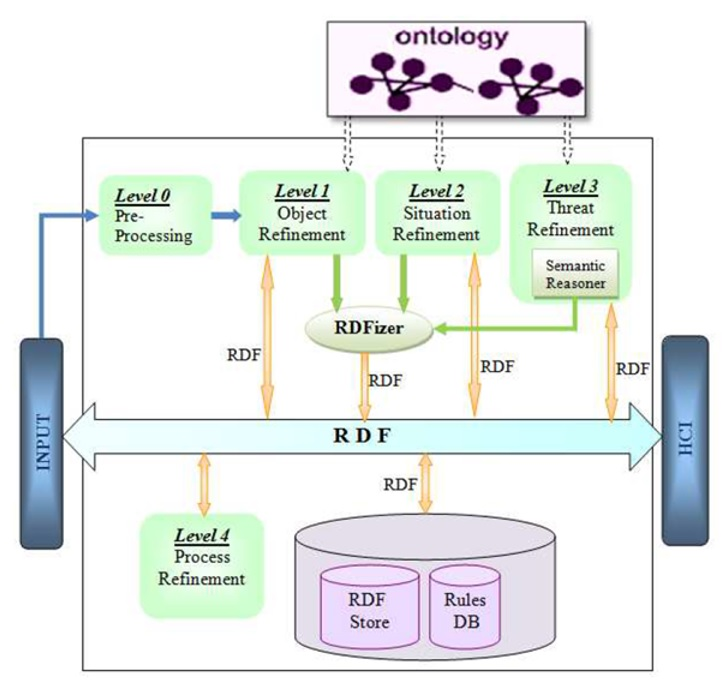
\includegraphics[width=\columnwidth]{Semantic_JDL.jpg}
  \caption{The semantic JDL model \cite{noughabi2013semfus}}
  \label{fig:semantidJDL}
\end{figure}


The semantic JDL model \cite{noughabi2013semfus} combines the basic JDL model with Semantic Web technologies.
The JDL semantic model in Figure \ref{fig:semantidJDL} is structured into several levels, each addressing different aspects of data processing. At Level 0, the focus is on preprocessing various data sources, resulting in cleaned data that is forwarded for object refinement without introducing any semantic elements. Level 1 involves transforming objects and their attributes into standard RDF format for storage. While this level includes tasks such as object identification, these processes rely on mathematical algorithms and image processing rather than semantic definitions. To effectively structure the data, predefined ontologies are necessary, allowing for the integration of attributes into the RDF format using an RDFizer, with the data stored in an RDF-Store database.
In Level 2, the model uses prior knowledge and environmental information alongside RDF data from Level 1 to define the situation of objects and their interrelationships. New relationships and previously unknown attributes are identified through inference, leading to updates in the RDF data that reflect any changes in information.
Level 3 emphasizes the evaluation of the current situation and the prediction of potential threats and vulnerabilities. A semantic reasoner plays a crucial role at this level, employing inference techniques to assess the situation and identify solutions and opportunities related to threats. The results of this analysis are converted into RDF format for storage.
Finally, Level 4 focuses on monitoring the system's performance and resource allocation. An expert evaluates the outputs from Level 3 to make informed decisions that enhance the overall efficiency of the system. The JDL semantic model operates with multiple databases, including one for RDF information and ontologies and another for rules. Proper database management principles must be upheld to ensure compatibility, prompt updates, and efficient data handling. Specific details regarding inputs and outputs may vary based on the domain of application.

One of the notable features of JDL, which makes it suitable for distributed architecture, is its ability to effectively separate tasks.
One of the advantages of the JDL fusion model over other fusion models is the separation of fusion stages into completely
distinct parts. This allows for the distribution of different components of the JDL model across various systems, 
enabling distributed fusion operations. 
Therefore, in this article, the JDL fusion model is utilized to present its distributed version 
for smart traffic application.


\subsection{Semantic Web in smart city}

Architectures of smart cities should combine data received from sensors in a manner that is readable by machines and publishable. To add meaning to the raw data generated by sensors and enhance data interaction and integration, Semantic Web technology has been employed. Semantic Web adds new information to the architectures of Internet of Things (IoT) for sensor fusion.



In \cite{article28}, the LSM architecture is introduced to achieve data interaction through the Semantic Web by integrating sensor data. It provides a user interface for publishing, annotating, and querying sensor data, utilizing the SSN ontology for describing sensor data and streams. The architecture links time-dependent data with external resources through semantic annotations, standardizes diverse data formats, and incorporates contextual knowledge from sources like DBpedia and GeoNames to enhance advanced querying.
This approach does not address query decomposition and distributed query execution and does not consider
  optimizing query execution. Additionally, it considers the execution of CQELS queries centrally and does not consider 
  the cost of sending data to the central node.


In \cite{Al-Baltah2020}, the SDFF framework is proposed to integrate data from heterogeneous sensors using Semantic Web technologies to resolve inconsistencies, such as differences in measurement units. It consists of layers for raw data collection, storage (separate repositories for raw and semantic data), semantic annotation, conflict resolution, and data dissemination. The framework ensures accurate data fusion and comparison, offering a comprehensive solution for managing and harmonizing diverse sensor data.
This article does not discuss topics such as distributed processing and query execution, query execution optimization, processing of large streaming data, and prevention of sending data to only one central node (centralized approach).


In \cite{Samadian2014}, a framework is introduced to combine and aggregate heterogeneous data streams from sensors, 
transforming them into feature streams to reduce data volume and increase efficiency.
 In \cite{inproceedings31}, sensor data is converted into RDF based on domain ontologies, 
 focusing on reducing transmitted data and optimizing bandwidth, but it lacks discussion on query 
 processing and execution optimization.
  In \cite{article32}, the Sense2Web framework enhances data integration by semantically representing sensor features and linking them to external resources, facilitating seamless aggregation and system interaction.


In \cite{inproceedings33}, a novel architecture is introduced for aggregating heterogeneous sensor networks
 by converting sensor measurements into semantic data and using ontologies for 
 enhanced data aggregation. However, it does not cover a distributed three-layer 
 architecture for data collection, query processing, or bandwidth management.
  In \cite{Wang2017}, another architecture integrates heterogeneous IoT data with a
   data aggregation layer to unify and improve data quality. Although it enhances 
   data fusion at a central node, it lacks an optimized query processing model and 
   a distributed approach that could improve system performance.


The SIGHTED architecture \cite{article35} collects and disseminates sensor data but faces challenges due to its
 centralized approach. Annotated data is stored and queried later, which increases query response times. 
 Drawbacks include lack of query optimization, inability to handle large data streams, 
 and reliance on sending all data to a central node. In \cite{Zafeiropoulos2008},
  a semantic framework with three layers—data collection, processing, and a semantic 
  layer—ensures data consistency and annotation through ontologies. However, it lacks
   distributed processing and centralizes data, leading to inefficient query execution
    and no optimization for large data transmission. In \cite{belcao2020streaming}, 
    a framework utilizing Streaming Virtual Knowledge Graphs integrates semantic data 
    streams using OBDA. While effective for data integration, generating ontologies from
     RDBMS databases is time-consuming and inefficient for decentralized environments 
     like smart cities, lacking efficient query decomposition and execution capabilities.



In \cite{zappatore2023semantic}, the study addresses semantic interoperability challenges
 in smart cities where diverse IoT solutions generate large data volumes exchanged via APIs. 
 It highlights the role of ontologies and shared vocabularies to enhance environmental sensing 
 and wellness monitoring. By using sensor-agnostic APIs and ontology modules for mobile crowd-sensing,
  the framework improves data integration, scalability, and real-time responsiveness in IoT applications.
   Privacy concerns in smart cities are addressed by the 'Ontology-Based Privacy-Preserving' (OBPP) framework \cite{GHEISARI20211},
    which uses ontologies and semantic reasoning to tackle heterogeneity, privacy, and service provision.
     Additionally, Semantic Web technologies play a key role in Agriculture 5.0 by improving data interoperability, 
     accessibility, and real-time operations in the agricultural sector \cite{de2023spatio}.    





\subsection{Fog Computing architectures}


Cloud computing offers extensive resources for handling complex tasks in smart cities \cite{Garca2011ExploringTL},
 but it has limitations such as high latency, lack of contextual awareness, and inadequate mobility support,
  which impede real-time processing. Edge computing addresses these issues by extending cloud capabilities to 
  the network edge, providing localized processing and storage to reduce latency and improve bandwidth efficiency,
   making it ideal for real-time smart city services \cite{Ahmed2017BringingCC}, \cite{Rahman2019BlockchainAI}.
    Additionally, cloud and fog computing are explored to bring cloud resources closer to the edge,
     enhancing the performance of smart city systems \cite{Abbas2018MobileEC}.




Perera \cite{Perera2017FogCF} explores real-world fog computing applications in agriculture, healthcare, and transportation
 but does not cover Semantic Web-based approaches. In \cite{Hu2017SurveyOF}, fog and edge computing are compared with cloud computing
  in smart environments, focusing on privacy, energy consumption, and challenges, but without integrating Semantic
   Web solutions. Shi \cite{Shi2016EdgeCV} highlights the benefits and challenges of edge computing, including privacy 
   and service optimization, through case studies, but lacks Semantic Web integration. Recent research on fog 
   computing and the Internet of Everything (IoE) \cite{Baccarelli2017FogOE} addresses latency reduction and 
   resource constraints, emphasizing scalability and real-time capabilities but provides limited detail on
    smart city applications. In \cite{Giordano2016SmartAA}, a three-layer architecture called Rainbow
     uses intelligent agents in smart city IoT systems but omits Semantic Web technology for data fusion.
      In \cite{inproceedings61}, a tiered-edge architecture introduces semantic stream processing 
      for workload distribution but lacks ontology-based query decomposition and efficient sub-query handling.


 
FogBus \cite{TULI201922} is a framework for cloud-fog integration, improving performance by 
activating cloud resources during overload, but it lacks semantic data processing and query 
decomposition. The "Analytics Everywhere" architecture \cite{article63} uses edge, fog, and cloud layers
 for smart parking analytics but does not optimize user requests or use RDF for data fusion. A four-layer
  fog architecture \cite{Arkian2017} focuses on context awareness and low latency but 
  lacks Semantic Web and data fusion models. Dastjerdi's five-layer architecture \cite{Dastjerdi2016} misses a distinct 
  fog layer and fails to address semantic issues. In \cite{ortiz2022atmosphere}, a collaborative IoT architecture using agent-oriented algorithms
   and CEP does not support semantic or heterogeneous data processing. A CR edge processing platform \cite{bonte2023towards} improves
    cloud efficiency but lacks high-level query translation and load balancing strategies. Recent studies \cite{XHAFA2020730} highlight edge computing’s role
     in enhancing data quality through semantic enrichment and event processing in smart cities. To address data integrity challenges in fog computing, \cite{SELLAMI202464} 
     introduces a verification protocol using SIS and identity-based signatures, improving security and efficiency.



\subsection{RDF stream Processing appoaches}


Real-time processing of large data streams has led to the development of RDF stream processing (RSP) models
 and continuous querying languages aimed at addressing the challenge of heterogeneous data. Systems such
  as EP-SPARQL \cite{anicic2011ep}, SPARKWAVE \cite{komazec2012sparkwave}, and INSTANS \cite{rinne2012instans} utilize temporal operators,
   while others like C-SPARQL \cite{barbieri2010c} and CQELS \cite{le2011native} rely on sliding windows for continuous query execution.

RSP system implementations are generally categorized into distributed and centralized models. Distributed approaches, such as DRSS \cite{dia2018drss},
 built on the Apache Storm platform, and CQELS Cloud \cite{le2013elastic}, leverage frameworks like Spark Streaming,
  Flink, and Storm for parallel stream processing. While these models enhance scalability and parallel execution,
   they often introduce complexities in implementation, upgrading, and usage. Centralized models, including
    C-SPARQL \cite{barbieri2010c}, SparqlStream \cite{calbimonte2010enabling}, and SPARKWAVE \cite{komazec2012sparkwave}, 
    struggle with processing capacity and exhibit limitations in scalability, concurrent query handling, and collaboration.


MAS4MEAN \cite{mebrek2020stream} addresses the limitations of centralized models by adopting a multi-agent approach that parallelizes query processing 
through multiple instances of the C-SPARQL engine.
Despite its ability to manage large event volumes,
   MAS4MEAN faces challenges in accelerating complex queries, performing local query execution,
    and avoiding redundant sub-query execution, leading to bandwidth inefficiency and increased query times as data and query complexity grow.

While continuous query operators for SPARQL 
have been developed to address stream heterogeneity, challenges related to parallelization and scalability persist.
 Methods such as DIONYSUS \cite{gillani2016dionysus} and CQELS Cloud \cite{le2013elastic} focus on distributing and processing large-scale RDF
  streams in parallel. Efficient partitioning of queries and data across nodes, with minimal data exchange, remains essential for
   optimizing the processing of RDF data streams at scale.



The article \cite{dia2018drss} introduces a scalable distributed approach for RDF stream processing by
 leveraging query rewriting, partitioning, and RDF graph partitioning to minimize inter-node data exchange.
  However, it lacks a task assignment strategy and does not implement a master-worker framework, leaving some execution details unclear.

The Waves method \cite{khrouf2016waves} utilizes the Apache Storm framework to distribute C-SPARQL
 queries across nodes, effectively handling large data volumes. However, it does not incorporate query 
 decomposition, leading to redundant executions and inefficient query performance.

StreamQR \cite{calbimonte2016query} rewrites C-SPARQL queries into a Union of Conjunctive Queries (UCQ)
 based on ontology, injecting domain knowledge into the query. While this allows parallel execution, 
 it can create large queries with multiple unions, increasing execution costs without optimizing time window lengths or conditions.

Table \ref{tab:comparison} outlines various frameworks and their capabilities, including query decomposition, 
prevention of redundant query execution, and whether they employ a layered architecture.
 The DIVIDE platform \cite{de2024enabling} dynamically adapts IoT stream queries based on real-time contexts
  using Semantic Web technologies but focuses mainly on dynamic query adaptation, leaving some performance aspects dependent on network conditions.



%\onecolumn

\begin{table*}[h!]
  % \centering
  % \flushleft % Align the caption to the left
  % \caption*{\textbf{Summary of related works}} % Use caption* to remove the extra space
  % \caption{Summary of related works}

  % \caption{\hspace{-\leftmargin}Summary of related works} % Adjust horizontal position
  % \vspace{-0.5em} % Adjust vertical space to remove blank lines

  \captionsetup{justification=raggedright, singlelinecheck=false} % Left-align the caption
  \caption{\newline Summary of related works}
  \vspace{-1em} % Adjust this value to remove blank space if necessary



  \resizebox{\textwidth}{!}{%
  \begin{tabular}{lccccccc}
    \hline
      \textbf{Method} & \textbf{Query Decomposition} & 
      \textbf{Duplicate Query Execute} & \textbf{Handle Large Data Stream} &
       \textbf{Query Processing} & \textbf{DataType} & \textbf{Layered Architecture} &
       \textbf{Query Optimization}  \\ \hline
       Zafeiropoulos et al. 2008 \cite{Zafeiropoulos2008} & \ding{55} & - & \ding{55} & C & RDF & \ding{51} & \ding{55}  \\ 
       Patni et al. 2011 \cite{inproceedings31} & \ding{55} & - & - & C & RDF & \ding{55} & \ding{55}  \\ 
       De et al. 2012 \cite{article32}  & \ding{55} & - & - & C & RDF & \ding{55} & \ding{55}  \\ 
      Phuoc et al. 2012 \cite{article28} & \ding{55} & - & - & C & RDF & - & \ding{55}  \\ 
      Gyrard et al. 2013 \cite{inproceedings33} & - & - & - & C & RDF & \ding{55} & -  \\ 
      Nagib et al. 2016 \cite{article35} & \ding{55} & - & \ding{55} & C & RDF & \ding{55} & \ding{55}  \\ 
      Dastjerdi et al. 2016 \cite{Dastjerdi2016} & - & - & - & C & Non-RDF & \ding{51} & -  \\ 

      Giordano et al. 2016 \cite{Giordano2016SmartAA} & - & - & - & - & Non-RDF & \ding{51} & -  \\ 
      Khrouf et al. 2016 \cite{khrouf2016waves} & \ding{55} & \ding{51} & \ding{51} & D & RDF & \ding{55} & \ding{55}  \\ 
      Calbimonte et al. 2016 \cite{calbimonte2016query} & Syntactically & \ding{51} & \ding{51} & C & RDF & \ding{55} & \ding{55}  \\ 

      Wang et al. 2017 \cite{Wang2017} & \ding{55} & - & - & C & RDF & \ding{51} & \ding{55}  \\ 
      Arkian et al. 2017 \cite{Arkian2017} & \ding{55} & - & \ding{51} & D & Non-RDF & \ding{51} & \ding{55}  \\ 
      Dia et al. 2018 \cite{dia2018drss} & Syntactically & \ding{55} & \ding{51} & D & RDF & \ding{55} & \ding{51}  \\ 

      Tuli et al. 2019 \cite{TULI201922} & \ding{55} & - & \ding{51} & D & Non-RDF & \ding{51} & \ding{55}  \\ 
      Cao et al. 2019 \cite{article63} & \ding{55} & \ding{51} & \ding{51} & D & Non-RDF & \ding{51} & \ding{55}  \\ 

      Al-Baltah et al. 2020 \cite{Al-Baltah2020} & \ding{55} & - & - & C & RDF & - & \ding{55}  \\ 
      Mebrek et al. 2020 \cite{mebrek2020stream} & \ding{55} & \ding{51} & \ding{51} & D & RDF & \ding{51} & \ding{55}  \\ 

      Ortiz et al. 2022 \cite{ortiz2022atmosphere} & \ding{55} & - & - & D & Non-RDF & \ding{51} & \ding{55}  \\ 
      Bonte et al. 2023 \cite{bonte2023towards} & Syntactically & - & \ding{51} & D & RDF & \ding{51} & \ding{51}  \\ 
      \textbf{DiSIF (our solution)} &   \textbf{Semantically} & 
      \textbf{\ding{55}} &   \textbf{\ding{51}} &   \textbf{D} &   \textbf{RDF} &   \textbf{\ding{51}} &
      \textbf{\ding{51}}  \\ \hline
  \end{tabular}
}
  
  \label{tab:comparison}
  \vspace{1mm} % Optional: add space before the note
  \footnotesize{Note: C and D refer to "Centralized" and "Distributed", respectively}
\end{table*}




% \begin{figure*}
%   \centering

%   \includegraphics[width=0.5\textwidth]{AllinOneFrameWork_modified.drawio.pdf}
%   \caption{DiSIF framework}
%   \label{fig:overall}
% \end{figure*}

\begin{figure}[t]
  \centering
  % \includegraphics[width=\columnwidth]{AllinOneFrameWork_modified.drawio.pdf}
  \includegraphics[width=\columnwidth]{AllinOneFrameWork_modified.drawio.pdf}
  \caption{DiSIF framework}
  \label{fig:overall}
\end{figure}

%\twocolumn



%???????????????????????? end related workd ??????????????????





\section{DiSIF: Distributed Semantic Information Fusion framework}
In this section, we introduce the distribute version of semantic JDL model within the framework of a three- layer architecture that includes edge, fog and cloud layers. As case study, we examine this model on traffic detection problem.



\begin{figure*}
    \centering
  
    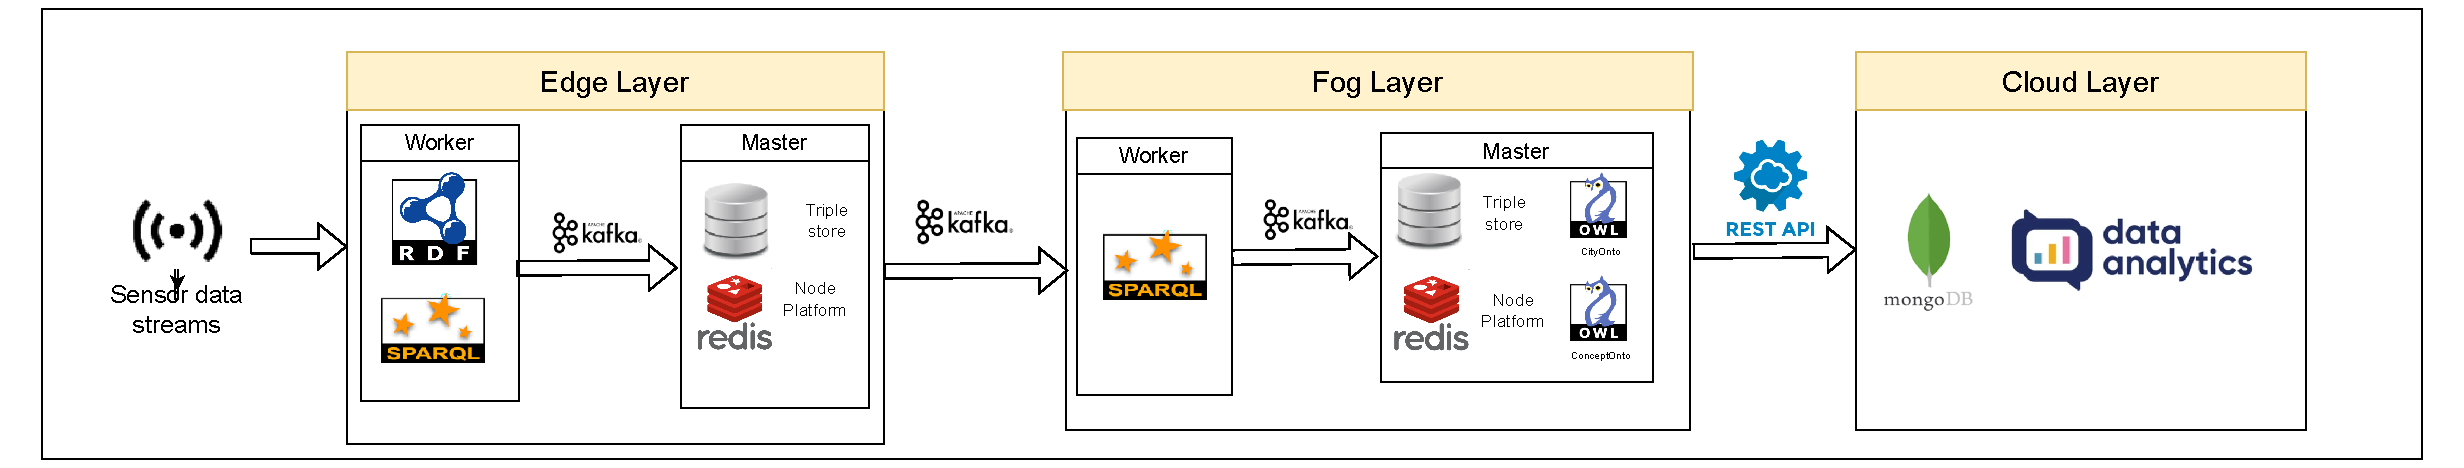
\includegraphics[width=1\textwidth]{Overall_Framework_Communication_OK.drawio.pdf}
    \caption{DiSIF Communication}
    \label{fig:overall_communication}
  \end{figure*}


\subsection{Overview of DiSIF Framework}

This section introduces the DiSIF framework, which consists of three layers: edge, fog, and cloud, designed for making time-sensitive and complex dependent decisions in IoT applications. 
As case study, we examine this model on traffic detection problem.

Next, the DiSIF framework's layers are examined from two perspectives: the JDL model and the fusion model.

\subsubsection{The JDL model perspective}







%\begin{figure*}
%  \centering
%  \includegraphics[width=0.8\textwidth]{C:/Users/Administrator/Desktop/Thesis_latex_Final/AllinOneFrameWork_modified.drawio.pdf}
%  \caption{The JDL model perspective}
%  \label{fig:framework1}
%\end{figure*}  

As illustrated in Figure \ref{fig:JDLandFusionprespective}, the DiSIF framework is organized into three layers: edge, fog, and cloud. Each layer consists of two types of nodes: worker nodes and master nodes. Worker nodes handle the reception and initial processing of data streams from the environment or lower layers, transmitting the results to the corresponding master node.

At the edge layer, the DiSIF framework operates at the first level of processing, known as object refinement, which is characterized by real-time decision-making and resource-efficient operations using minimal resources. The tasks performed in this layer align with the object refinement component of the JDL model.

The decisions made at the edge layer are then passed to the fog layer for more advanced processing and decision-making at the second level, known as situation refinement. This could include identifying traffic events or street congestion.

In the fog layer, decisions from the edge layer (level one) are aggregated using the cityOnto ontology to form new decisions at the fog level (level two). For more comprehensive, city-wide decisions at the third level (threat refinement), the results are sent to the cloud layer. The cloud layer stores all information and decisions from the lower layers in a database and performs intensive processing tasks, such as predicting traffic patterns and executing city-level management decisions. Thus, information processing, fusion, and decision-making occur progressively across each layer of the framework.


\subsubsection{The Fusion Model Perspective}


This section discusses the types of queries and fusion processes within the DiSIF framework,
 which supports efficient data processing across edge, fog, and cloud layers.

\textbf{Independent queries} in C-SPARQL can be executed in parallel without depending on other queries.
 These are suitable for tasks like counting vehicles in different areas, where subqueries can run simultaneously across multiple nodes.

 \textbf{Dependent queries} rely on results from previous queries, making them essential for complex,
  sequential operations like further analysis or data fusion.

In the DiSIF framework, data flows from the edge layer to the cloud layer, becoming more abstract and complex.
 The edge layer handles raw sensor data (level one), the fog layer processes information streams (level two), 
 and the cloud layer conducts large-scale decisions based on integrated data (level three).

The DiSIF framework, as illustrated in Figure \ref{fig:JDLandFusionprespective}, can be analyzed from the following aspects:

\textbf{Data Level}: The framework manages increasingly abstract data from sensors to city-wide information,
 with the edge layer focusing on sensor fusion and higher layers addressing broader queries, like traffic patterns.

\textbf{Query Types}: Independent queries are executed across layers and nodes in parallel, enhancing scalability.
Dependent queries run sequentially within a layer, where one query’s output serves as input for the next.

\textbf{Fusion Operations}: Vertical fusion aggregates data of the same type but on a larger scale (e.g., street-level data combined into area-wide traffic
 data). Horizontal fusion changes the concept of the data (e.g., transforming street congestion data into traffic-specific insights) 
 without altering its scale.

\textbf{JDL Model Alignment}: The DiSIF framework follows the JDL model, with object refinement at the edge layer,
 situation refinement in the fog layer, and threat refinement in the cloud layer, supporting layered, distributed decision-making.

This distributed approach improves data processing efficiency, scalability, and privacy, making it well-suited for smart city applications.
The subsequent section presents an overview of each layer in the DiSIF framework, aiming to deploy a Distributed Semantic JDL model.




% In this section, we first address the definition of the concepts of independent queries and dependent queries.
% \begin{itemize}
%  \item \textbf{Independent Query} 

% An independent query in C-SPARQL is a query that can be executed without dependence on the results of other queries. Additionally, it can be decomposed into independent subqueries, which can be executed in parallel without any interdependency, enabling efficient and scalable data processing. The results of these subqueries are separate from each other and can be executed and obtained without any connection to each other. An example of such a query is to investigate the number of vehicles present in a specific area. This query can be divided into subqueries that count the number of vehicles on the streets within that area. Each subquery can be executed independently, and the results can be published separately.

%     \item \textbf{Dependent Query}

%  A dependent query in C-SPARQL is a query that relies on the results of one or more previous C-SPARQL queries for its execution. Dependent C-SPARQL queries are usually used to perform operations such as analysis or further processing on the results of previous queries. This is essential for complex data analysis tasks involving sequential or fusion operations on RDF data streams.

% \end{itemize}

\begin{figure}[t]
    \centering
    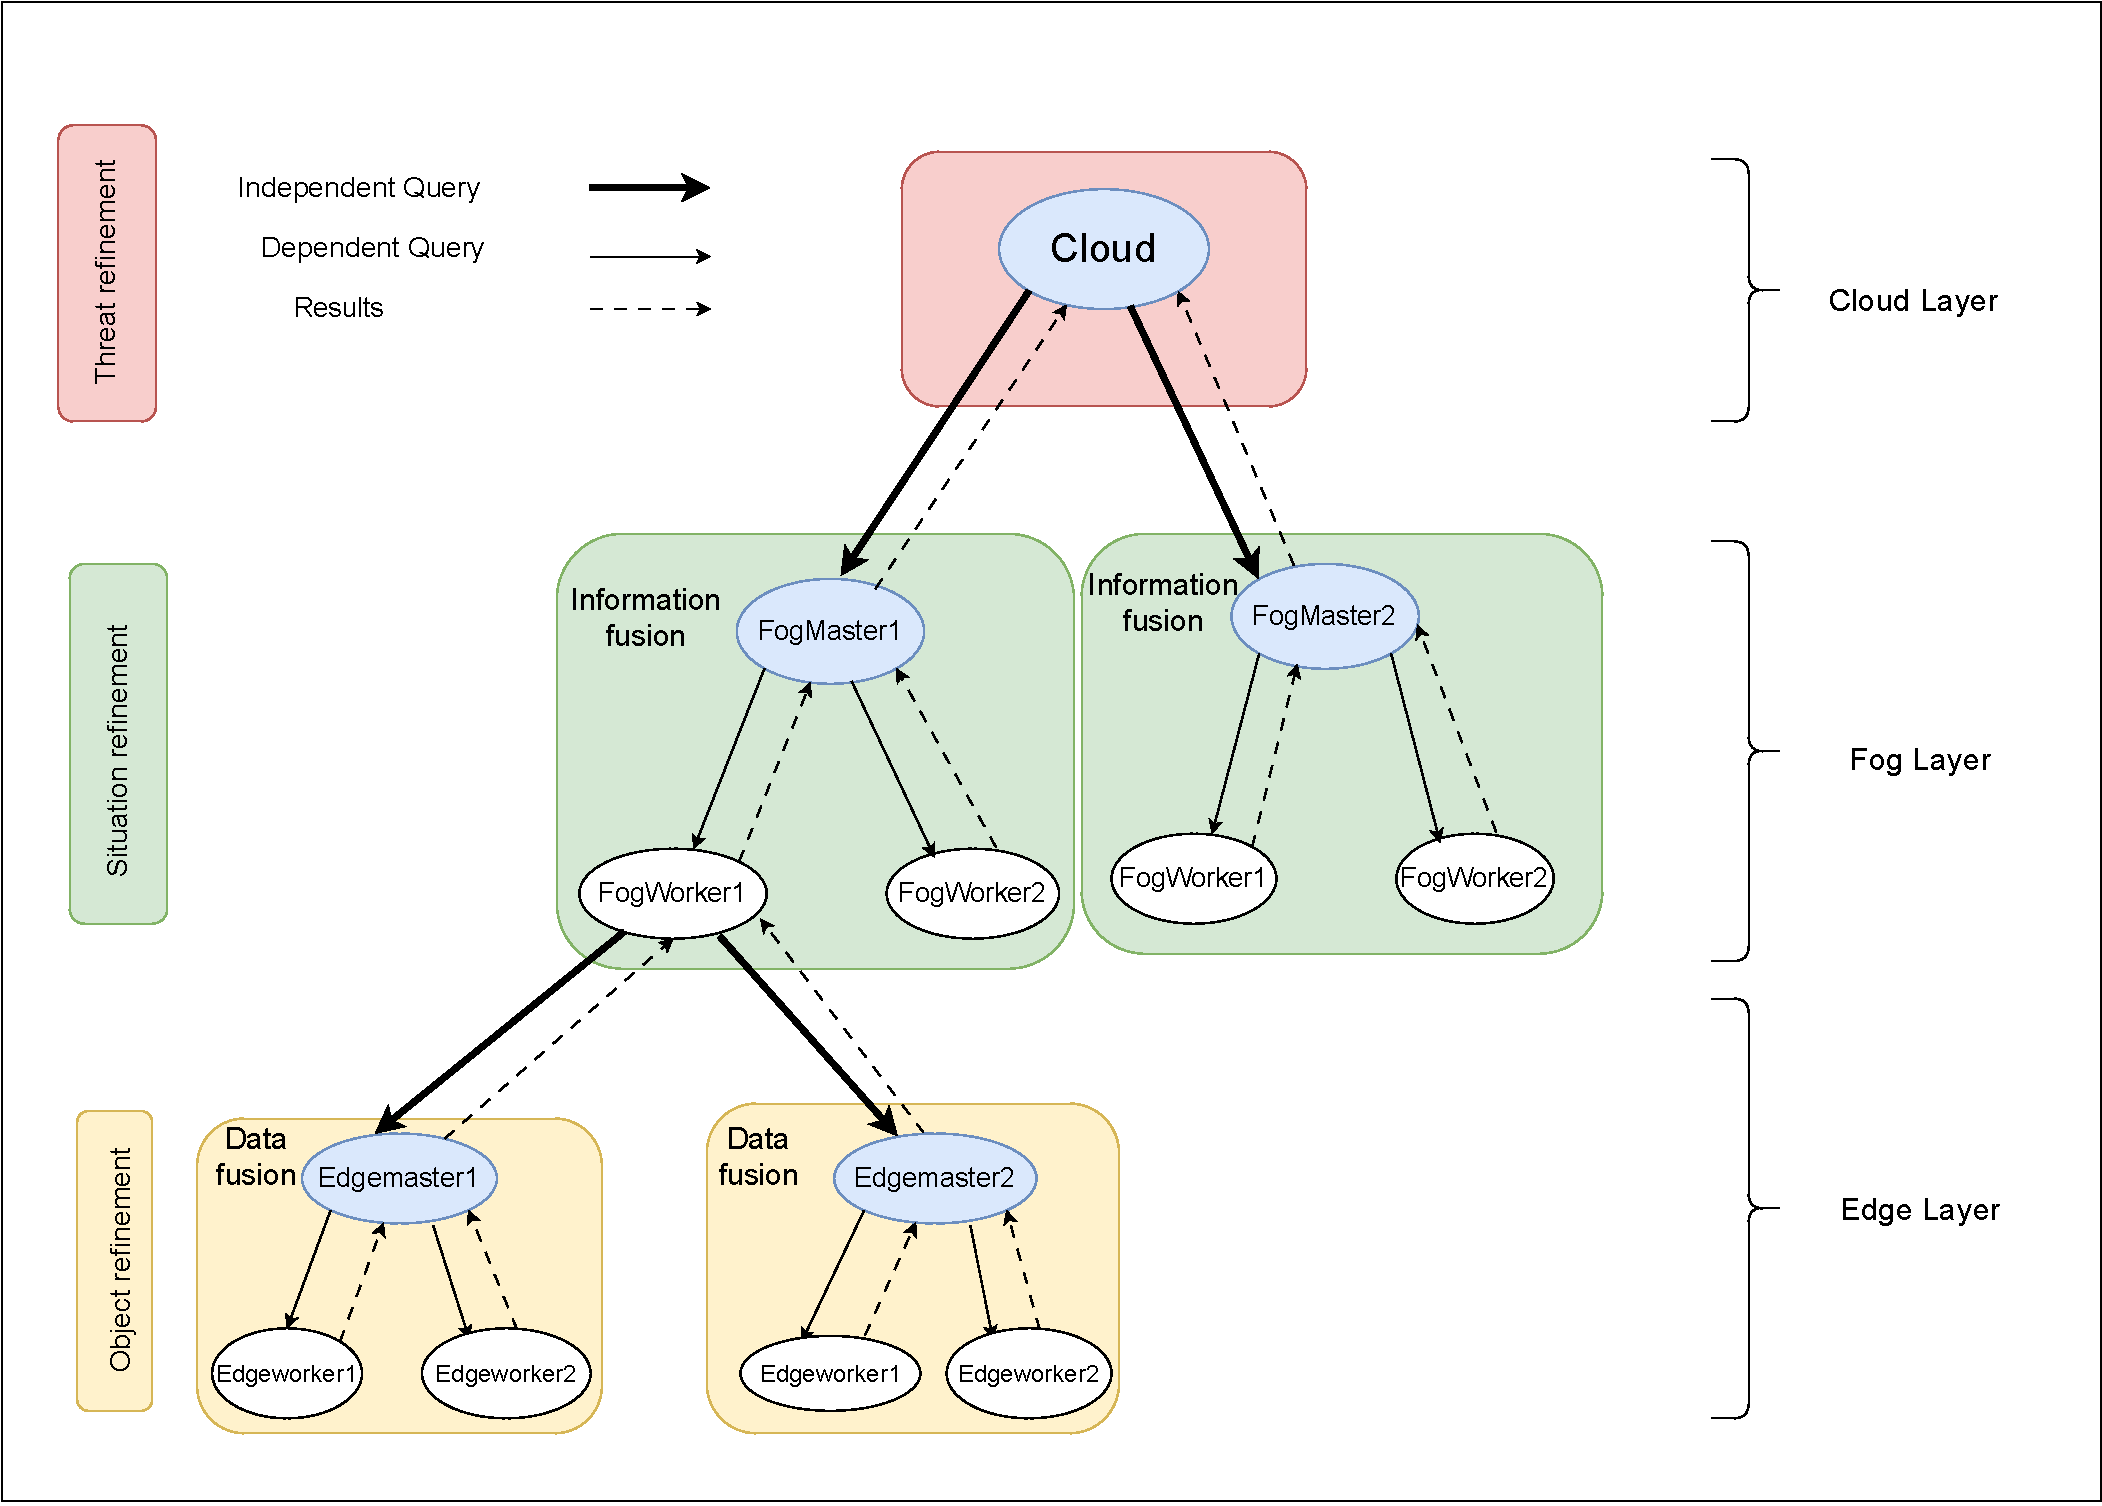
\includegraphics[width=\columnwidth]{h3.drawio.pdf}
    \caption{The JDL and fusion model perspectives}
    \label{fig:JDLandFusionprespective}
  \end{figure}

  
% \begin{figure*}
%   \centering
%   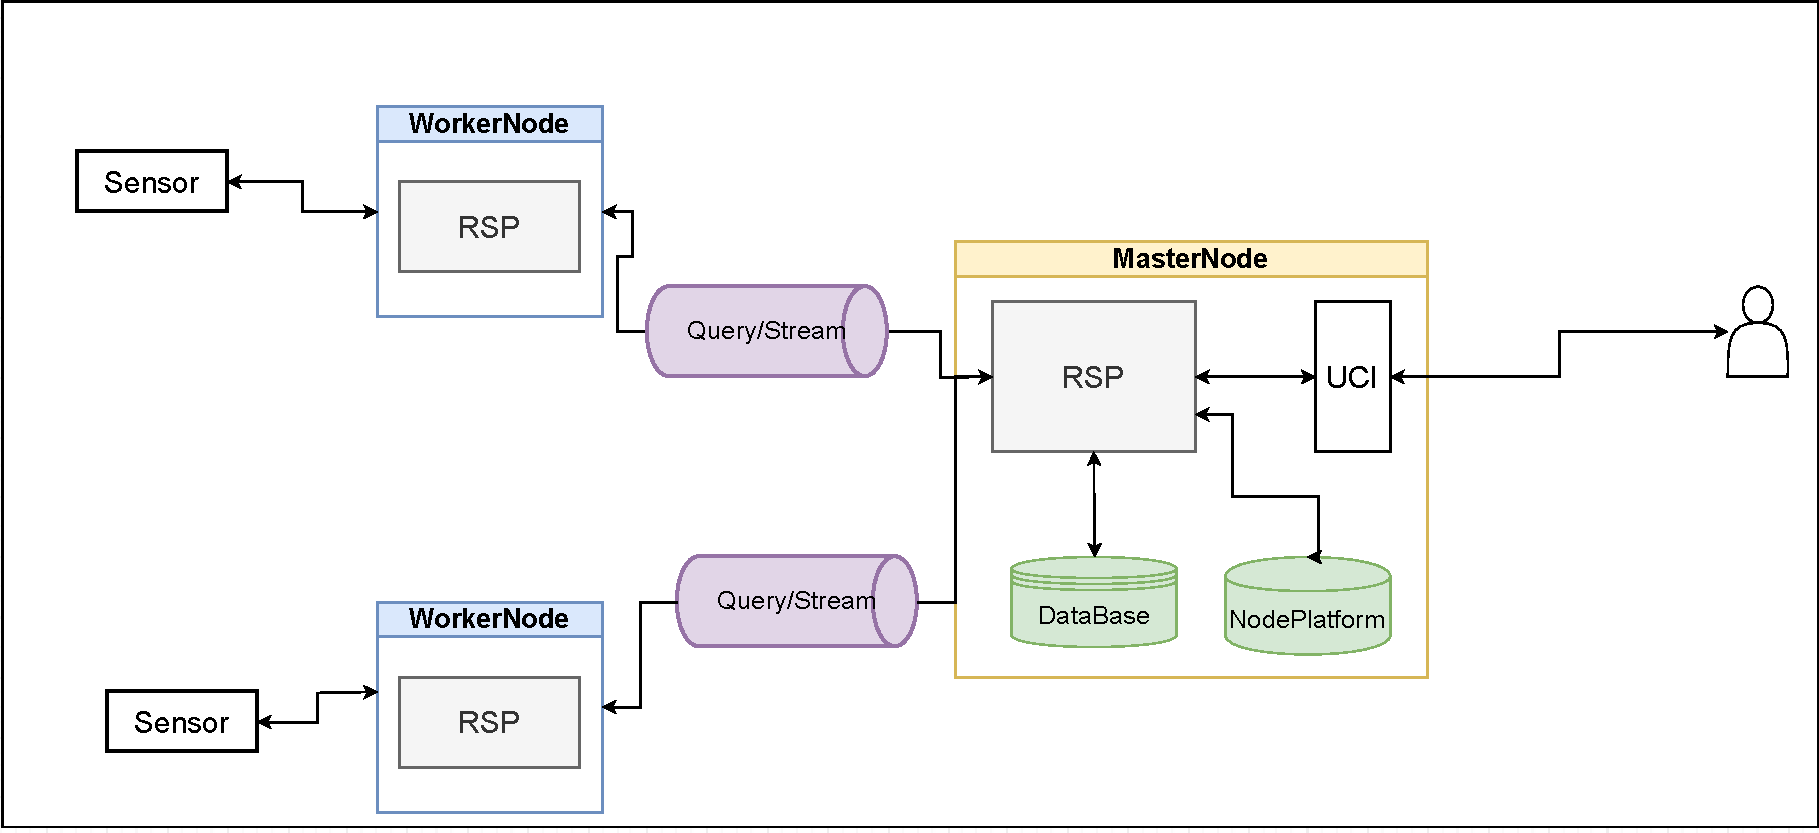
\includegraphics[width=0.5\textwidth]{EDgeLayer.drawio.pdf}
%   \caption{The Edge Layer}
%   \label{fig:edgelayer}
% \end{figure*}


% \begin{figure*}[ht]
%   \centering
%   \begin{minipage}{0.49\textwidth}
%       \centering
%       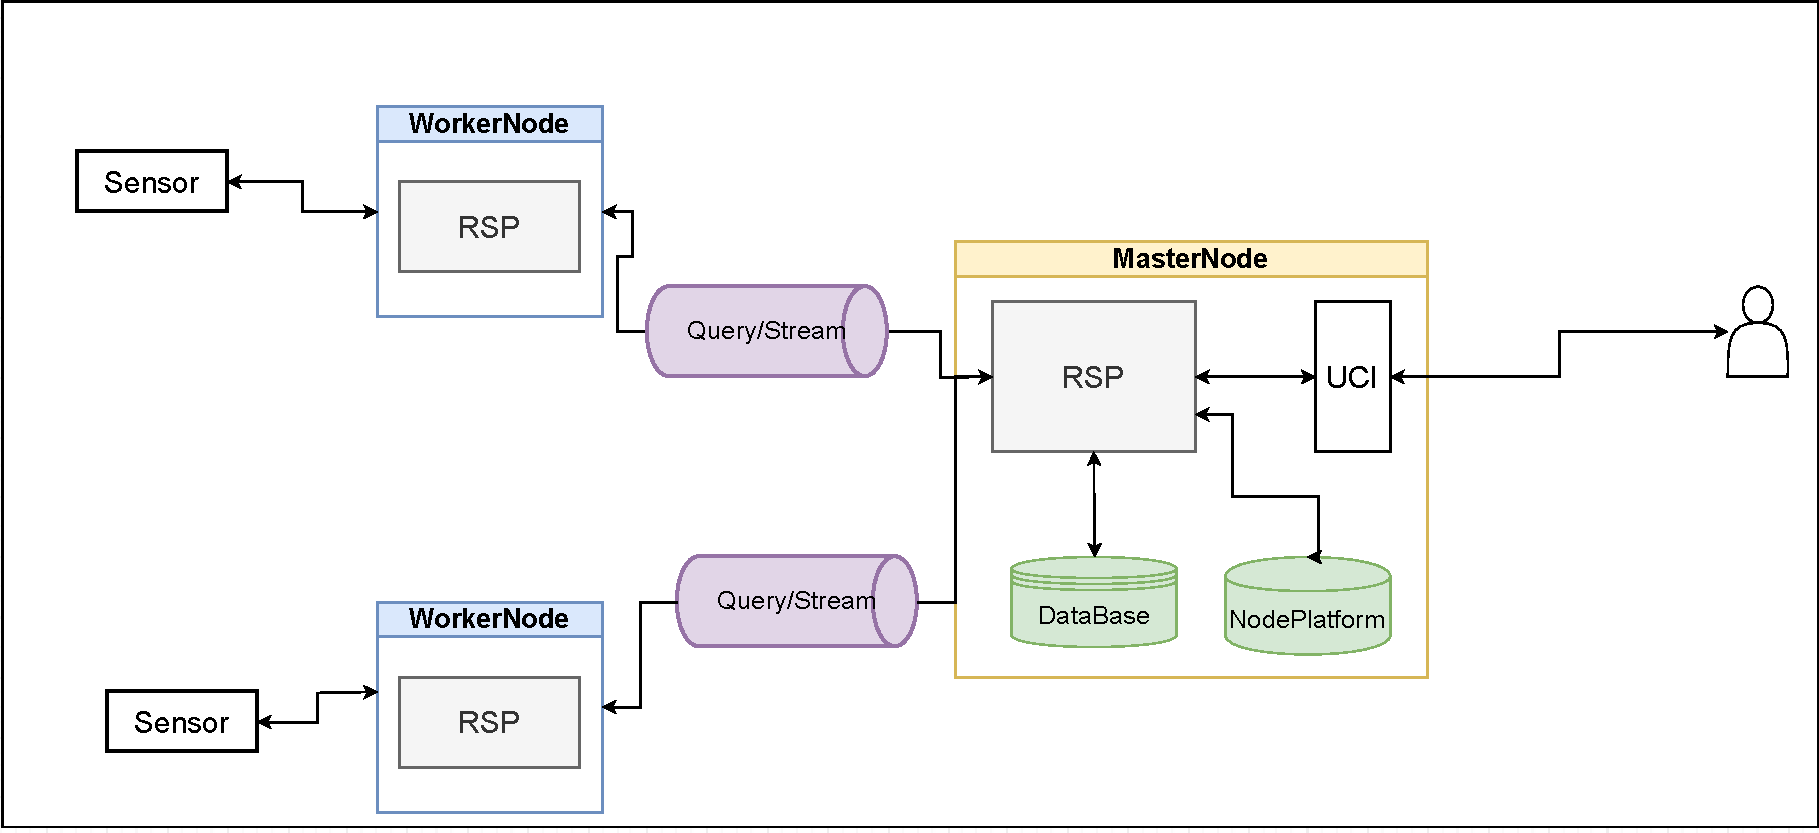
\includegraphics[width=\textwidth]{EDgeLayer.drawio.pdf}
%       \caption{The Edge Layer}
%       \label{fig:edgelayer}
%   \end{minipage}
%   \hfill
%   \begin{minipage}{0.49\textwidth}
%       \centering
%       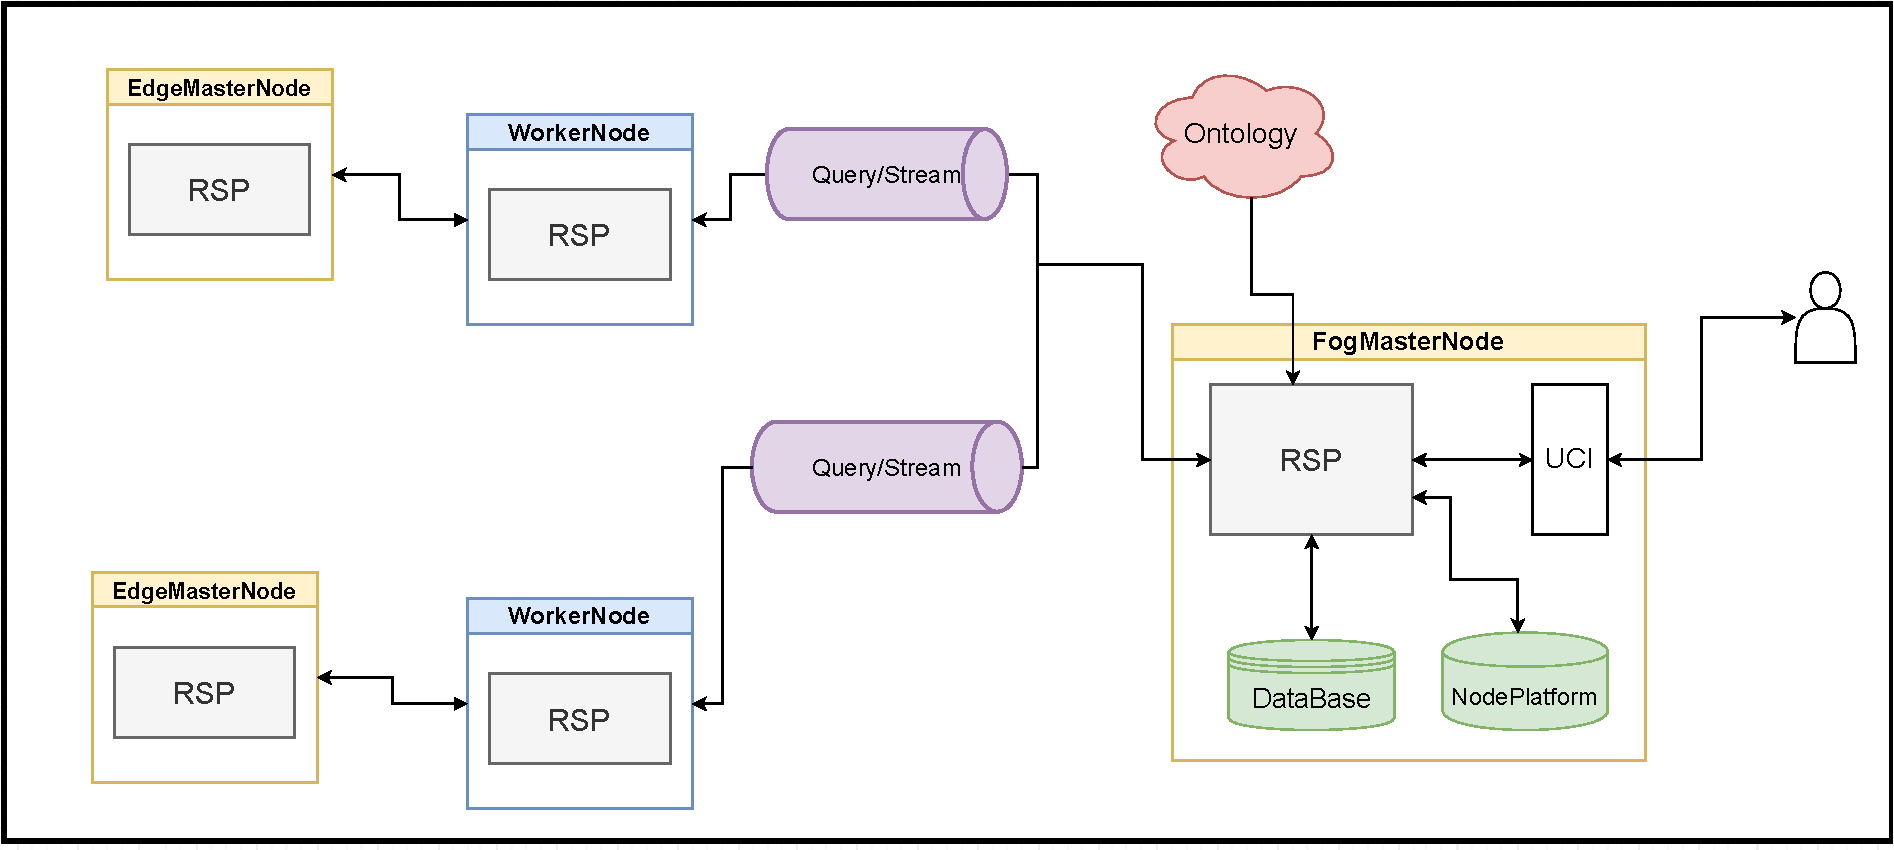
\includegraphics[width=\textwidth]{FogLayer.drawio.pdf}
%       \caption{The Fog Layer}
%       \label{fig:foglayer}
%   \end{minipage}
% \end{figure*}


\begin{figure}[t]
  \centering
  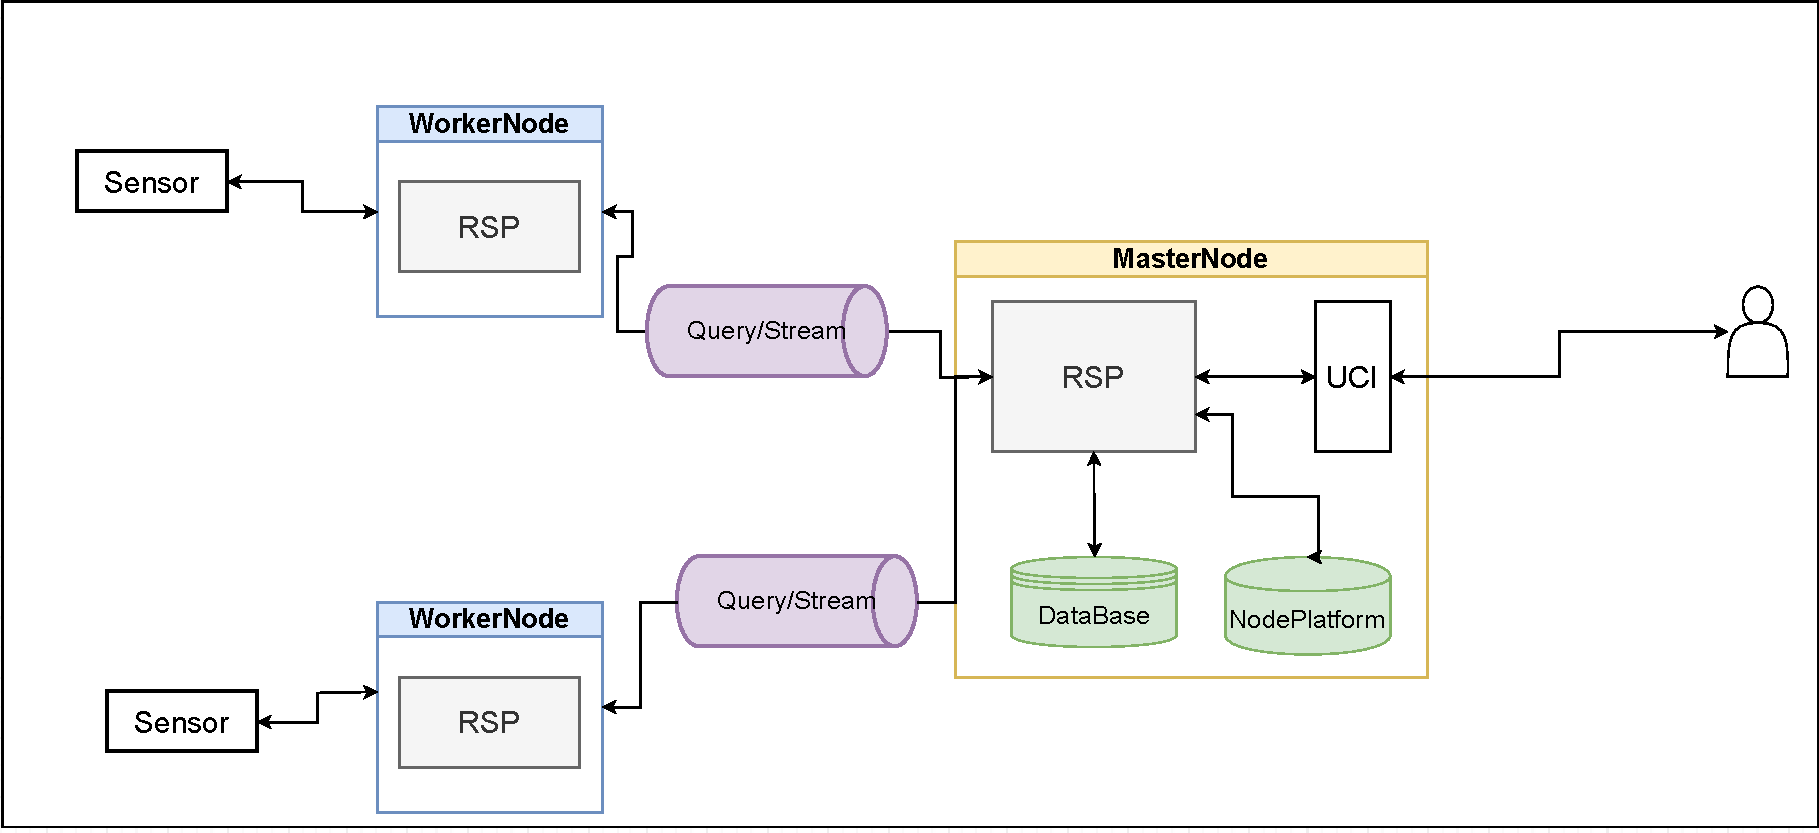
\includegraphics[width=\columnwidth]{EDgeLayer.drawio.pdf}
  \caption{The Edge Layer}
  \label{fig:edgelayer}
\end{figure}

\begin{figure}[t]
  \centering
  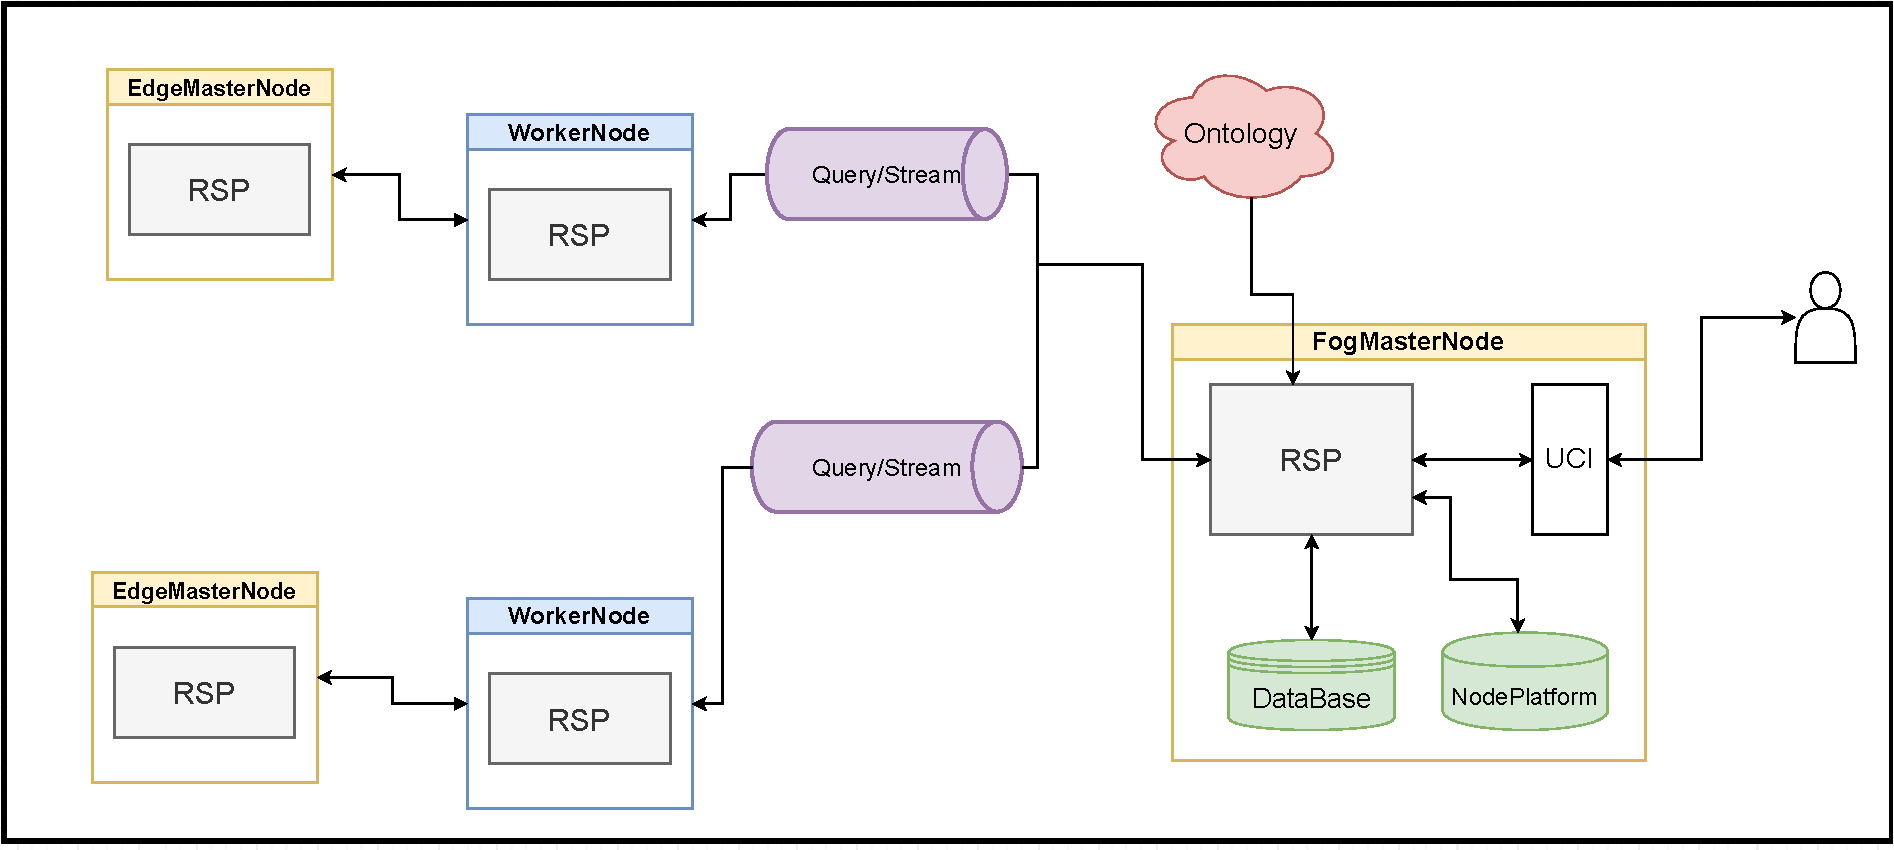
\includegraphics[width=\columnwidth]{FogLayer.drawio.pdf}
  \caption{The Fog Layer}
  \label{fig:foglayer}
\end{figure}


\begin{figure}[t] % Use [t] to attempt to place the figure at the top of the page
  \centering
  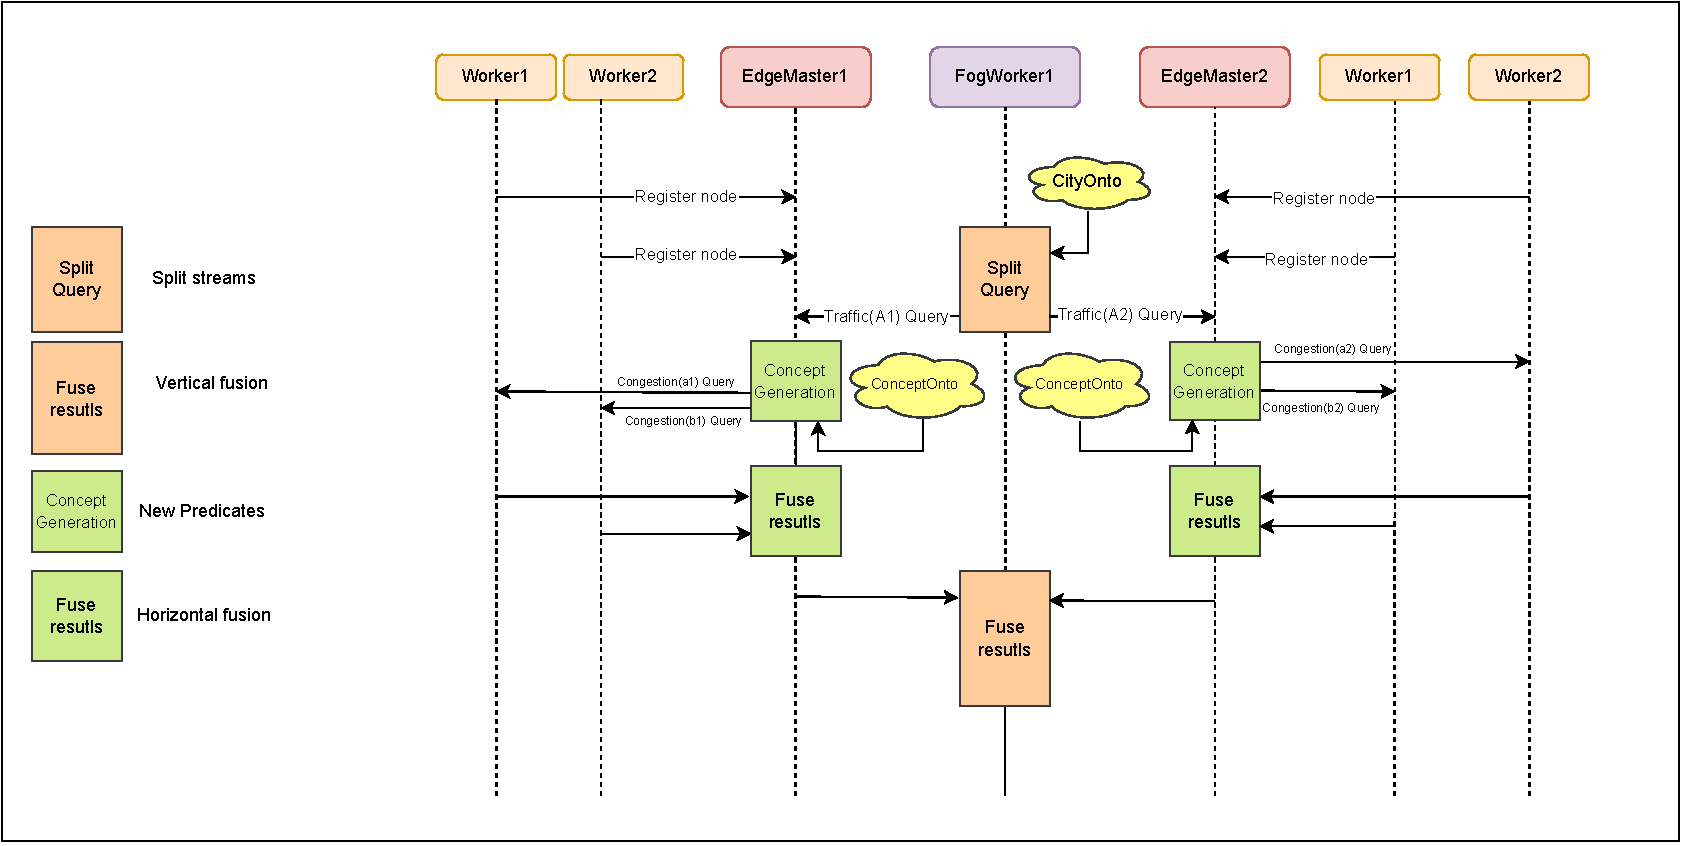
\includegraphics[width=\columnwidth]{Communication_new.drawio.pdf}
  \caption{Query execution request flow}
  \label{fig:queryexe}
\end{figure}


% The DiSIF framework, as illustrated in Figure \ref{fig:JDLandFusionprespective}, can be analyzed from the following aspects:

% \begin{itemize}
%     \item \textbf{Data Level}

% The designed framework is structured to manage data across distinct layers, transitioning from the edge layer to the cloud layer. The nature of the data becomes increasingly abstract, and its contextual complexity rises. At the edge layer, the data primarily comprises sensor data (Level one). In the fog layer, the data transforms into processed data or information streams. Queries performed at the edge layer focus on sensor data and involve operations related to data fusion. As queries progress to higher levels, they address broader concepts, such as traffic patterns, utilizing nodes in the fog layer for information fusion.

%     \item \textbf{Independent/Dependent Queries} 

% Queries defined in the DiSIF framework can be categorized into independent and dependent queries.
% Independent queries are usually inter-layer queries that can be executed simultaneously across multiple nodes, 
% with their results combined afterward. These queries are assigned from worker nodes in the upper layer to master nodes in the lower layer.


% Dependent queries, on the other hand, are intra-layer queries that must be executed sequentially and consecutively. The results of one
%  query are considered as input for another query. These queries are executed between worker and master nodes within a layer.
    

% \begin{figure*}
%   \centering
%   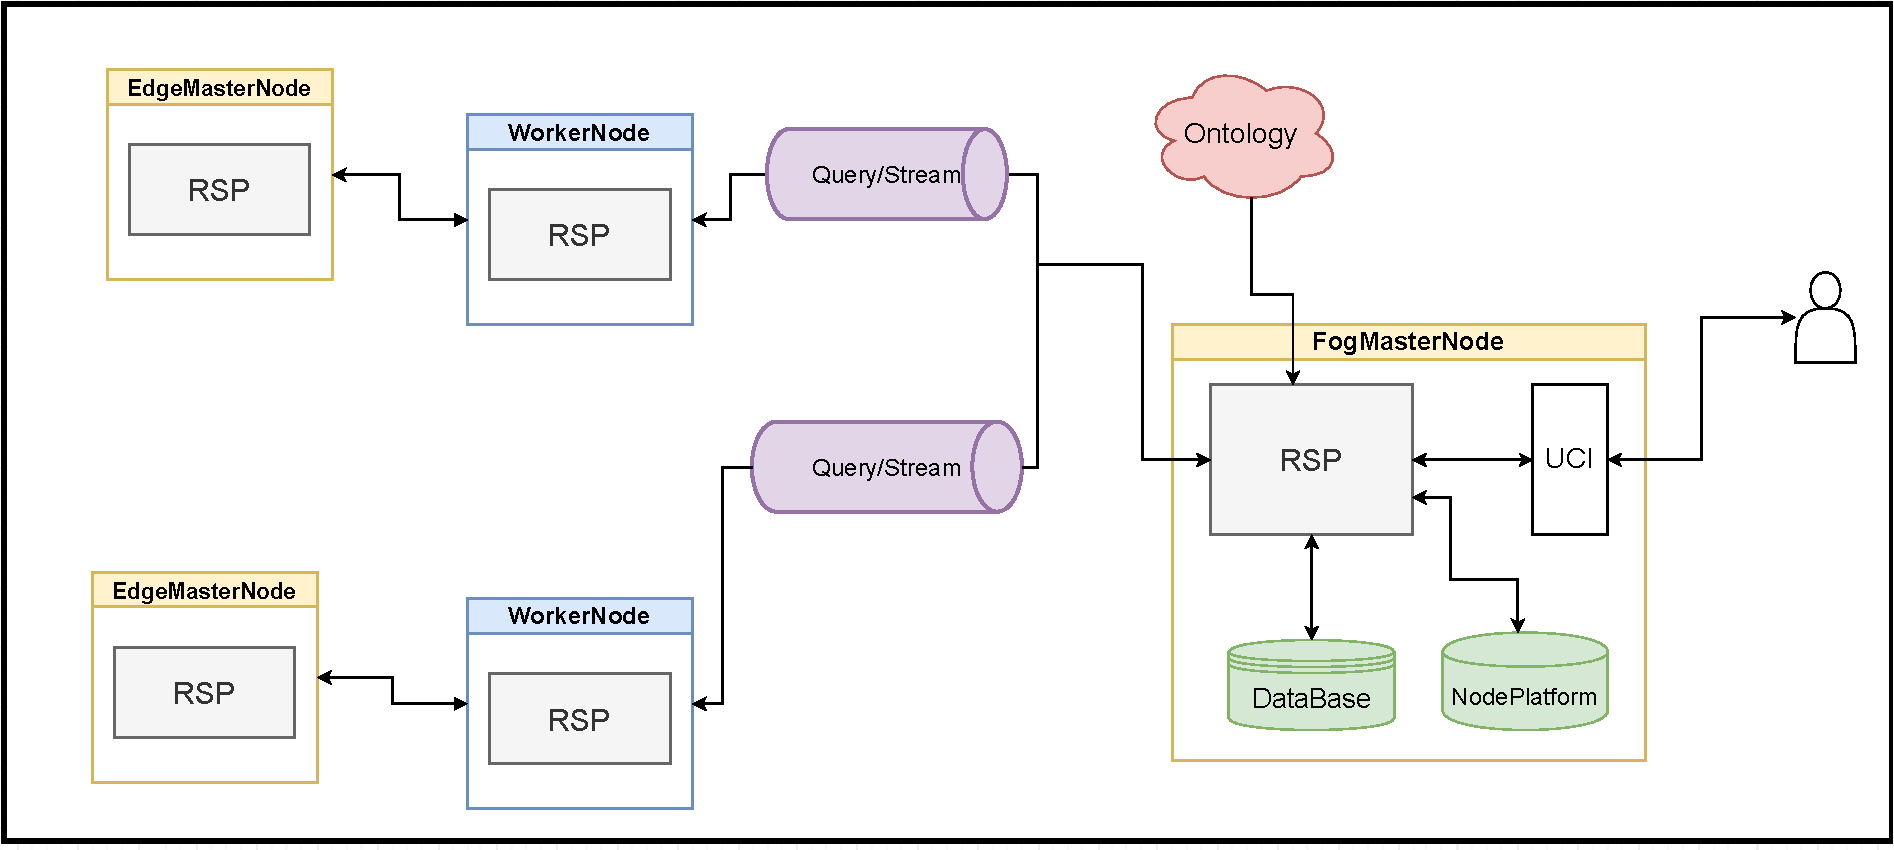
\includegraphics[width=0.5\textwidth]{FogLayer.drawio.pdf}
%   \caption{The Fog Layer}
%   \label{fig:foglayer}
% \end{figure*}


%     \item \textbf{Vertical vs. Horizontal Fusion} 


% Vertical fusion operations, resulting in an increase in the scale of the data.
%  In other words, the input and output of vertical fusion represent the same concept,
%   differing only in size and scale. For example, traffic data from multiple streets can be fused to generate traffic data for an entire area.



% Horizontal fusion, results in a change in the concept of the data. For instance, it involves fusing congestion data from a street to generate traffic data specific to that street. In this type of fusion, only the concept of the output data changes, while the scale and size of the data remain unchanged. Horizontal fusion can occur within each layer and between master and worker nodes.


    
%     \item \textbf{JDL Model Components}

%  In the DiSIF framework, the edge layer handles operations related to the JDL 
%  object refinement component, while situation refinement can be performed in the 
%  fog layer on the data received from the edge layer. Similarly, in the cloud layer, threat refinement operations can take place.
% \end{itemize}



% The subsequent section presents an overview of each layer in the DiSIF framework, aiming to deploy a Distributed Semantic JDL model.


% # node platform



\subsection{Edge Layer}






An overall view of the DiSIF framework for the Edge layer is depicted in Figure \ref{fig:edgelayer}.


In the Edge Layer, processing and fusion operations are performed on the streams of data from sensors.
 In the worker node, operations such as receiving data from sensors, executing queries assigned by the master node,
  and sending result streams back to the master are carried out. In the master node, operations involve
   receiving user queries via UCI, storing data in the database, registering and retrieving information about
    worker nodes in the NodePlatform, executing and assigning queries to worker nodes,
     receiving and aggregating received streams from worker nodes.



\section*{NodePlatform}



\begin{table}[t]
  % \centering

  \captionsetup{justification=raggedright, singlelinecheck=false} % Left-align the caption
  \caption{\newline Example of NodePlatform}
  \vspace{-1em} % Adjust this value to remove blank space if necessary


  % \captionsetup{justification=raggedright} % Left-align the caption
  % \caption{Example of NodePlatform} % Move caption above the tabular
  \begin{tabular}{cccc}
  \hline
  \textbf{Node} & \textbf{Concept} & \textbf{Location} & \textbf{Master} \\
  \hline
  $N^w_1$ & $Congestion$ & $loc1$ & $N^m_1$ \\
  $N^w_1$ & $Congestion$ & $loc2$ & $N^m_1$ \\
  $N^w_2$ & $Traffic$    & $loc3$ & $N^m_3$ \\
  $N^w_3$ & $Congestion$ & $loc5$ & $N^m_2$ \\
  \hline
  \end{tabular}
  \label{tab:NodePlatformTbl}
  \end{table}


  % #=================


  % #===========
The Node Platform as shown in Table \ref{tab:NodePlatformTbl} facilitates the registration of worker nodes
 with their corresponding master nodes, capturing essential information for each worker node
  such as its name,  the concepts it generates, the locations or streams it can produce 
  along with its corresponding master node.
   It is instrumental in breaking down queries into sub-queries, dispatching these sub-queries to 
   the appropriate worker nodes, and receiving result streams back at the master node.

Within the master node, the NodePlatform serves as a repository for information about registered 
worker nodes, allowing for easy retrieval and discovery of nodes associated with specific concept and location.

This functionality ensures that queries are directed to the correct node that generating specific concept for 
corresponding location.



The database component is used to store data and received streams from worker nodes. The stored data is utilized for query execution in the master node. The UCI component receives queries from users and sends them to the master node. It also returns the results of query execution from the master node to the user. Therefore, all user operations are performed through UCI.
In the master node, horizontal fusion operations on data (object refinement) from the Edge layer are conducted. Ultimately, the generated streams are sent to the worker nodes in the Fog layer.
Algorithm 1 outlines the assignment procedure of a worker node to the master node.



% \begin{algorithm*}
% \caption{RegisterWorkerNode}\label{register_worker_node}
% \begin{algorithmic}[1]
%     \Procedure{RegisterWorkerNode}{\textit{workerNode}}
%     \State\textit{WorkerNode} publish \textit{joinRequest} message with metadata to Kafka
%     \State Receive \textit{joinRequest} message at \textit{masterNode}
%     \State \textit{masterNode} store \textit{workerNode}'s metadata in \textit{Nodeplatform}
%     \State \textit{masterNode} send \textit{joinResponse} message to \textit{workerNode} with \textit{masterNode} information
%     \State Receive \textit{joinResponse} at \textit{workerNode} and store \textit{masterNode}'s information
%     \EndProcedure
% \end{algorithmic}
% \end{algorithm*}

\begin{algorithm}
  \caption{RegisterWorkerNode}\label{register_worker_node}
  \begin{algorithmic}[1]
      \Procedure{RegisterWorkerNode}{\textit{workerNode}}
      \State\textit{WorkerNode} publish \textit{joinRequest} message with metadata to Kafka
      \State Receive \textit{joinRequest} message at \textit{masterNode}
      \State \textit{masterNode} store \textit{workerNode}'s metadata in \textit{Nodeplatform}
      \State \textit{masterNode} send \textit{joinResponse} message to \textit{workerNode} with \textit{masterNode} information
      \State Receive \textit{joinResponse} at \textit{workerNode} and store \textit{masterNode}'s information
      \EndProcedure
  \end{algorithmic}
  \end{algorithm}




The metadata information sent from the worker node to the master node is contained:
the name of \textit{workerNode}, set of concepts that the \textit{workerNode} can 
generate
, the locations/streams it can produce along with its corresponding master node.


%\section*{Metadata Information:}

%\begin{itemize}
%    \item URL address related to \textit{workerNode}.
%    \item Resources of \textit{workerNode}.
%    \item Set of conceptual predicates that the workerNode can generate (\textit{predicate}s of \textit{workerNode}).
%    \item \textit{streamIRI} (identifiers of streams that \textit{workerNode} can inspect and process).
%\end{itemize}

\subsection{Fog layer}








An overall view of the DiSIF framework for the Fog layer is illustrated in Figure \ref{fig:foglayer}.
In the Fog layer, the data in the form of concept streams (instead of data stream) are processed and fused. Similar to the Edge layer, the operations of a worker node in the Fog layer include receiving concept streams from the Edge Layer and executing assigned queries from the master node.

In the master node of the Fog layer, operations involve receiving user queries via UCI, storing data in the database, registering and retrieving information about worker nodes in the NodePlatform, executing and assigning queries to worker nodes, receiving data streams from worker nodes, and fusing received streams from worker nodes.

The components in this layer are similar to those in the Edge Layer.
 For vertical fusion in the fog layer, particularly in the context of intelligent traffic, 
 the cityOnto ontology is essential. In this layer, this ontology serves as external data.




In the master node, horizontal fusion enables the completion
of situation refinement operations, and the resulting streams are forwarded to the cloud layer
 for extensive processing. 


Algorithm ~\ref{alg:QueryresponsemasterNode} outlines the query response process within the master node.
In this algorithm, the operations performed on the master node for processing user
 queries. It handles two types of queries: SPARQL queries (line 4) for answering static queries based on
  the data in the database (DB), and CSPARQL queries (line 6) for responding to queries over data streams.
  In line 7, the algorithm checks whether the concepts used in the query have already been 
  registered by any node within the NodePlatform. 
  If the corresponding node exists, in line 8, the location/stream of that node is compared with the one 
  in the query. If the required locations in the query have been previously registered for that node, 
  the query is divided into sub-queries based on the different locations (if necessary), 
  and each sub-query is forwarded to the corresponding nodes. The results are then gathered and 
  aggregated by the master node (lines 9 to 11).



In Algorithm \ref{alg:conceptQuery}, if the corresponding node for the concept and location extracted
 from the user's query is found, the operations for retrieving data from that node (line 6),
  executing the query, and returning the results (lines 7–8) are carried out. If node not found,
   in (line 10), one of the nodes that have been previously defined in the NodePlatform for the corresponding
   master node and for the requested
    location/stream is selected.
Then, in lines 11 and 12, based on the ConceptOnto ontology, all the necessary elements for
 constructing a query to generate the new concept are extracted, and in line 13,
  this query is generated using Algorithm \ref{alg:constructquery}.
Finally, in line 14, the NodePlatform is updated to include the new concept
 for the node and the specified location, and in line 15, the constructed query is sent
  to the selected node for execution.

  








\subsection{Cloud layer}
In the cloud layer, considering the received streams from the fog layer, semantic fusion operations on the streams take place. Threat refinement at a macro level are conducted in this layer. 
Global concept streams received from the fog layer are stored in a database, where predictions are made based on this data. In the cloud layer, heavy processing is performed periodically or as needed on historical data, with the results reported to the user. One significant task in this context is traffic prediction, 
which forecasts traffic in various locations at a macro level using both the stored data and ongoing streams from the fog layer.

\subsection{Query Execution Request Flow}


As depicted in Figure \ref{fig:queryexe}, one FogWorker and two EdgeMaster nodes, labeled $FogWorker1$,
 $EdgeMaster1$, and $EdgeMaster2$, are present. Initially,
  edge worker nodes perform the registration and storage of their metadata in the NodePlatform of the EdgeMasters.
   In this manner, all streams that these worker nodes can generate, along with the concepts (query predicates)
    they can execute, are stored in the EdgeMaster nodes.

A query is submitted through FogWorker1, which refers to two independent subqueries,
 $Traffic(A1)$ and $Traffic(A2)$, derived from the CityOnto ontology. 
These subqueries are executed in parallel on two separate locations/streams, $A1$ and $A2$,
 using $EdgeMaster1$ and $EdgeMaster2$. 


 \begin{figure}[t] % Use [t] for top placement
  \centering
  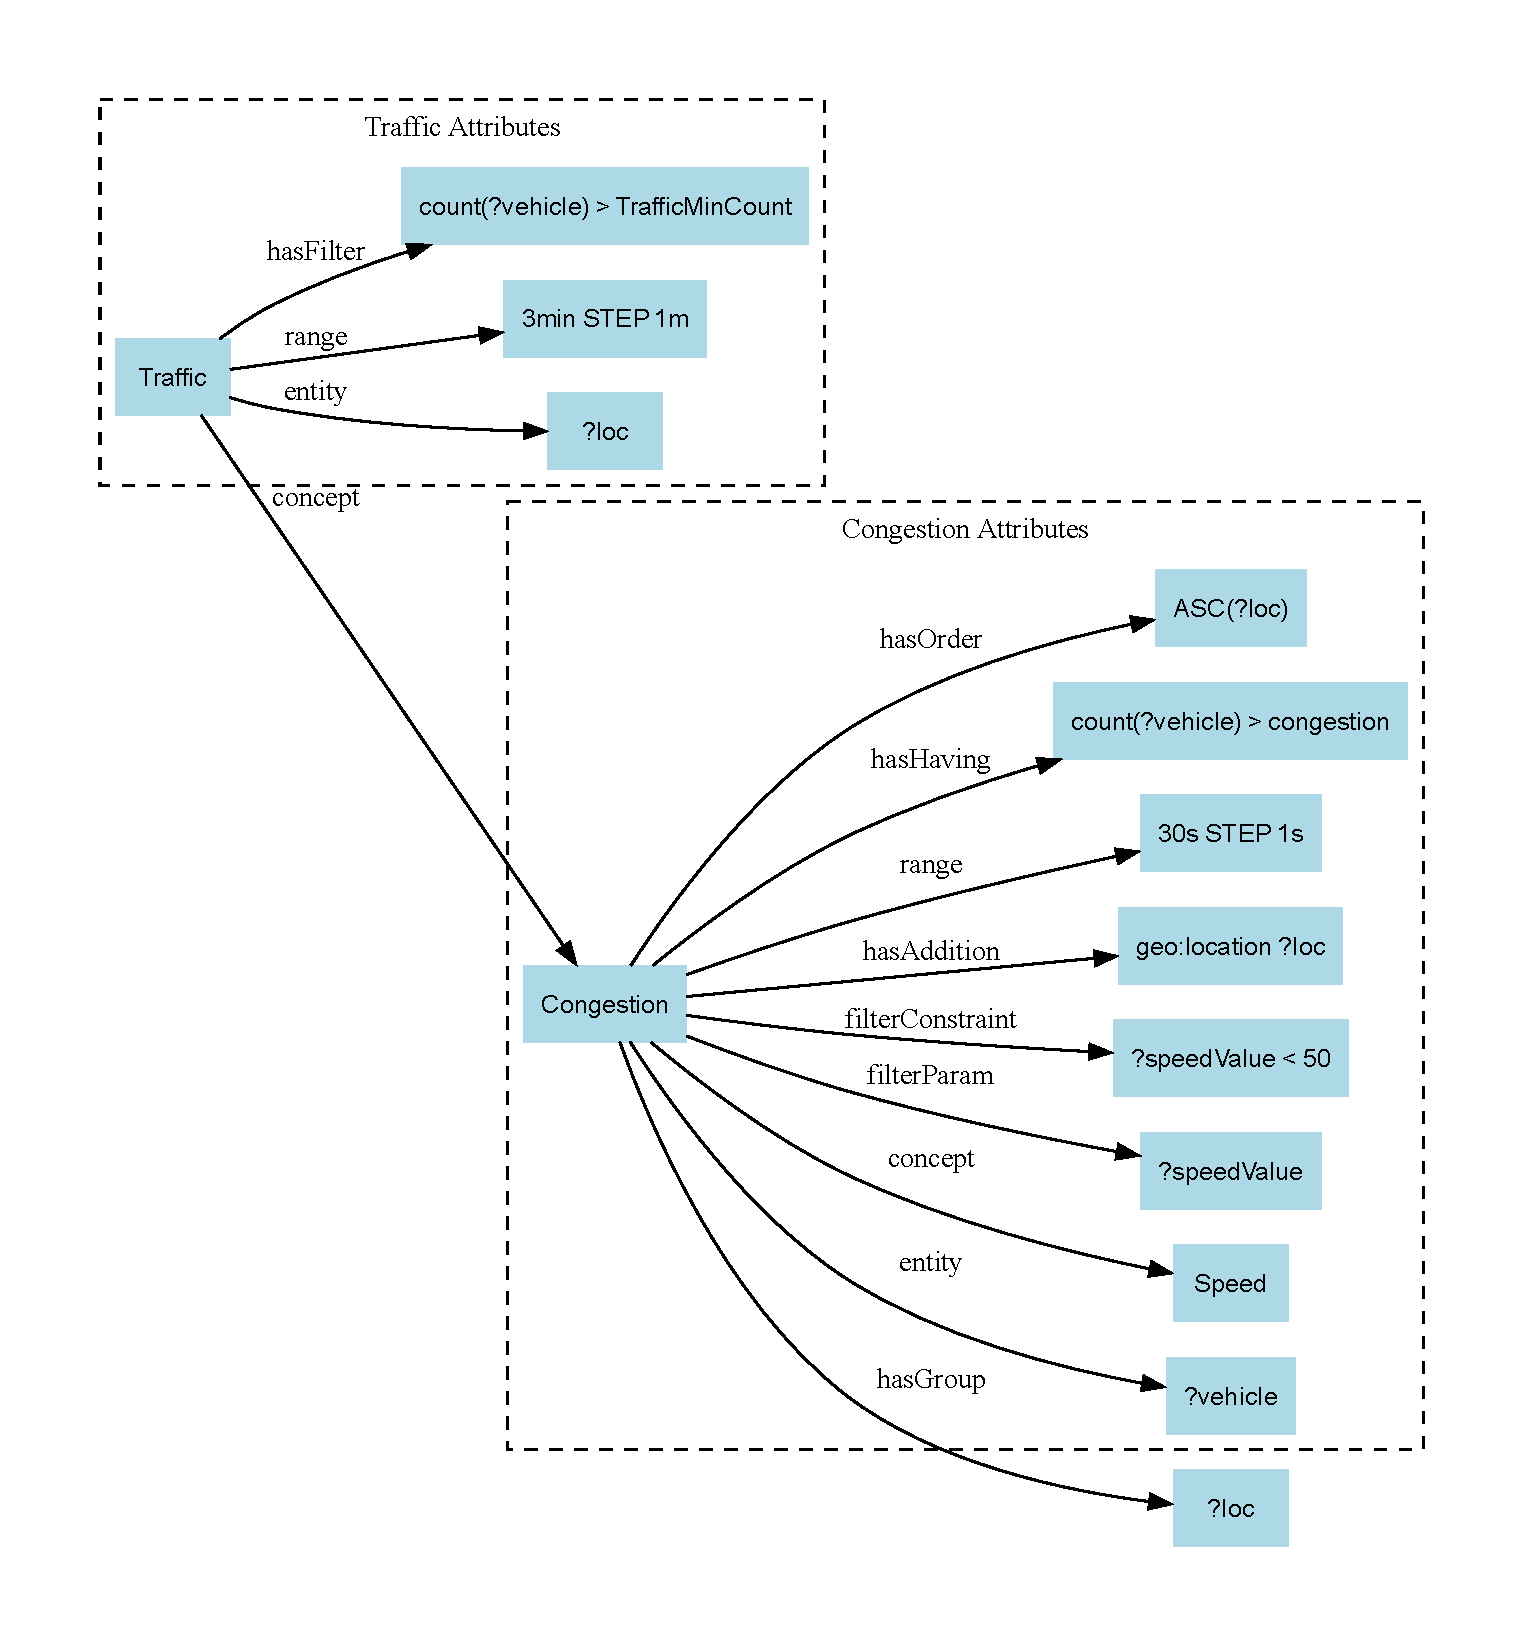
\includegraphics[width=\columnwidth]{ConceptOnto_GraphViz_new.pdf}
  \caption{Concept Ontology}
  \label{fig:conceptonto}
\end{figure}

In the EdgeMaster nodes, the concept generation component (Algorithm \ref{alg:constructquery}) utilizes
 the ConceptOnto ontology (Figure \ref{fig:conceptonto}) to generate concepts that do not have incoming streams.
  This process produces dependent subqueries, such as $Congestion(a1)$ and $Congestion(b1)$.
These sub-queries are then executed on edge worker nodes, and the results are returned to the EdgeMaster node. 

% Horizontal fusion is performed in the Fuse results component of EdgeMasters nodes,
%  and the results are referred back to $FogWorker1$.
% Within the Fuse results component from $FogWorker1$, vertical fusion is carried out combining the outputs 
% of queries on streams $A1$ and $A2$, resulting in the final output.

Horizontal fusion is conducted within the Fuse results component of the EdgeMasters nodes,
 with the results subsequently transmitted back to $FogWorker1$.
  Within the Fuse results component of $FogWorker1$, vertical fusion is executed by integrating the outputs of queries from streams $A1$ and $A2$, 
  ultimately yielding the final output.



\begin{figure}[t]
  \centering
  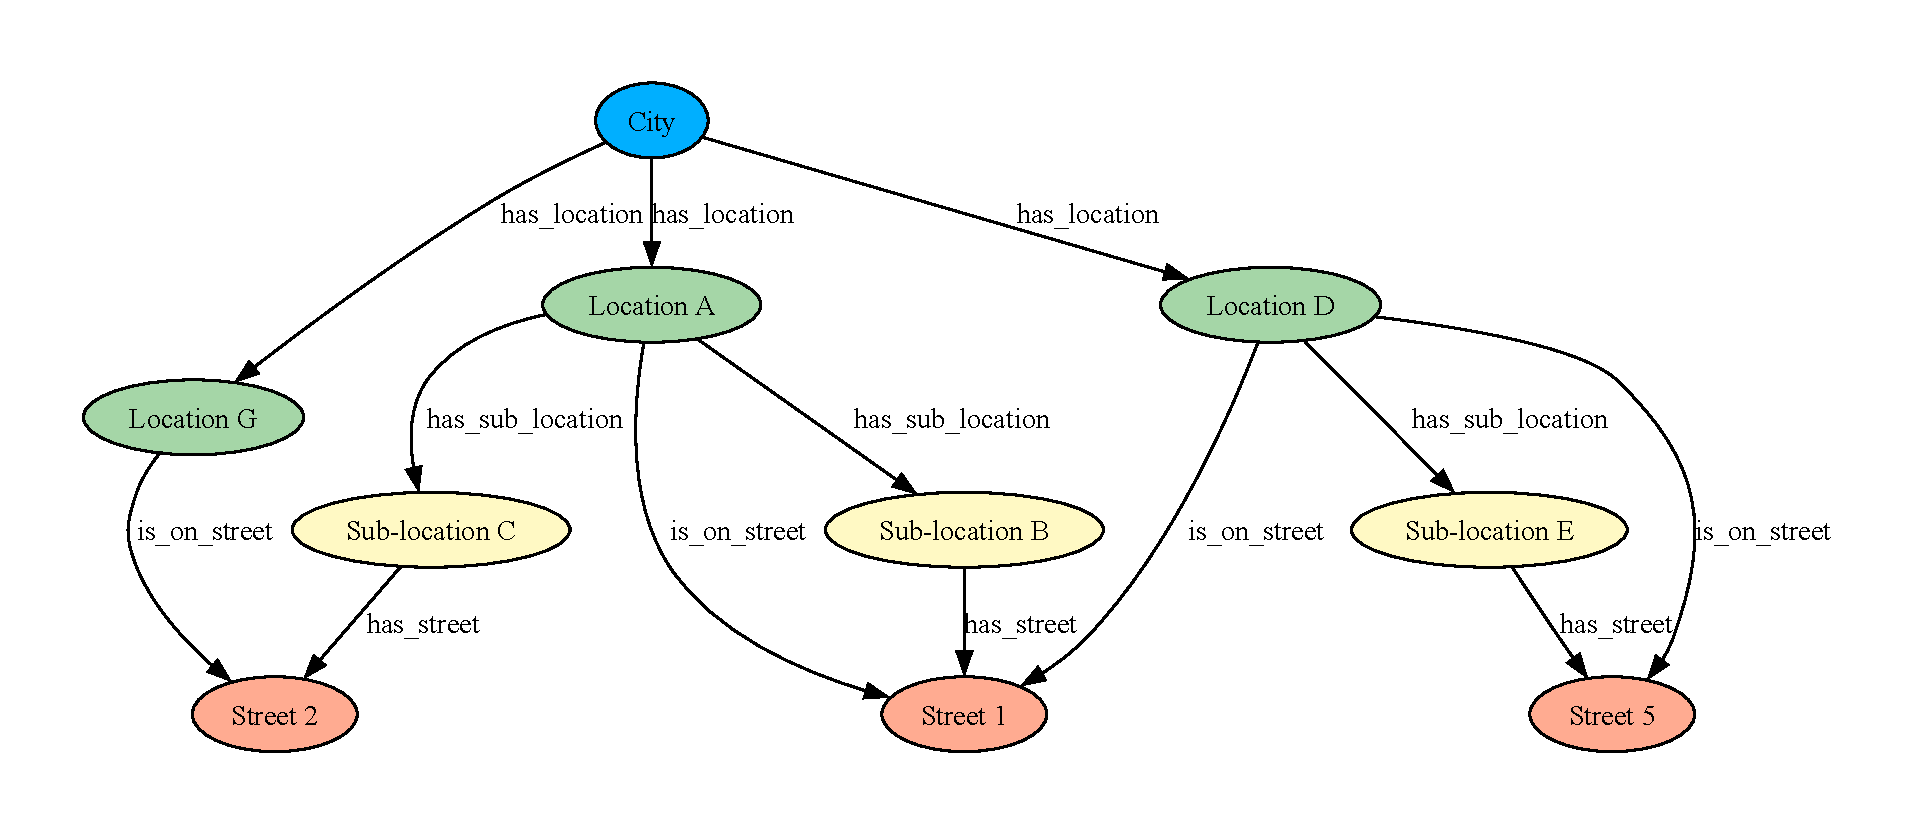
\includegraphics[width=0.5\textwidth]{cityOnto_graph.pdf}
  \caption{CityOnto example}
  \label{fig:CityOnto}
\end{figure}

\begin{figure}[t]
  \centering
  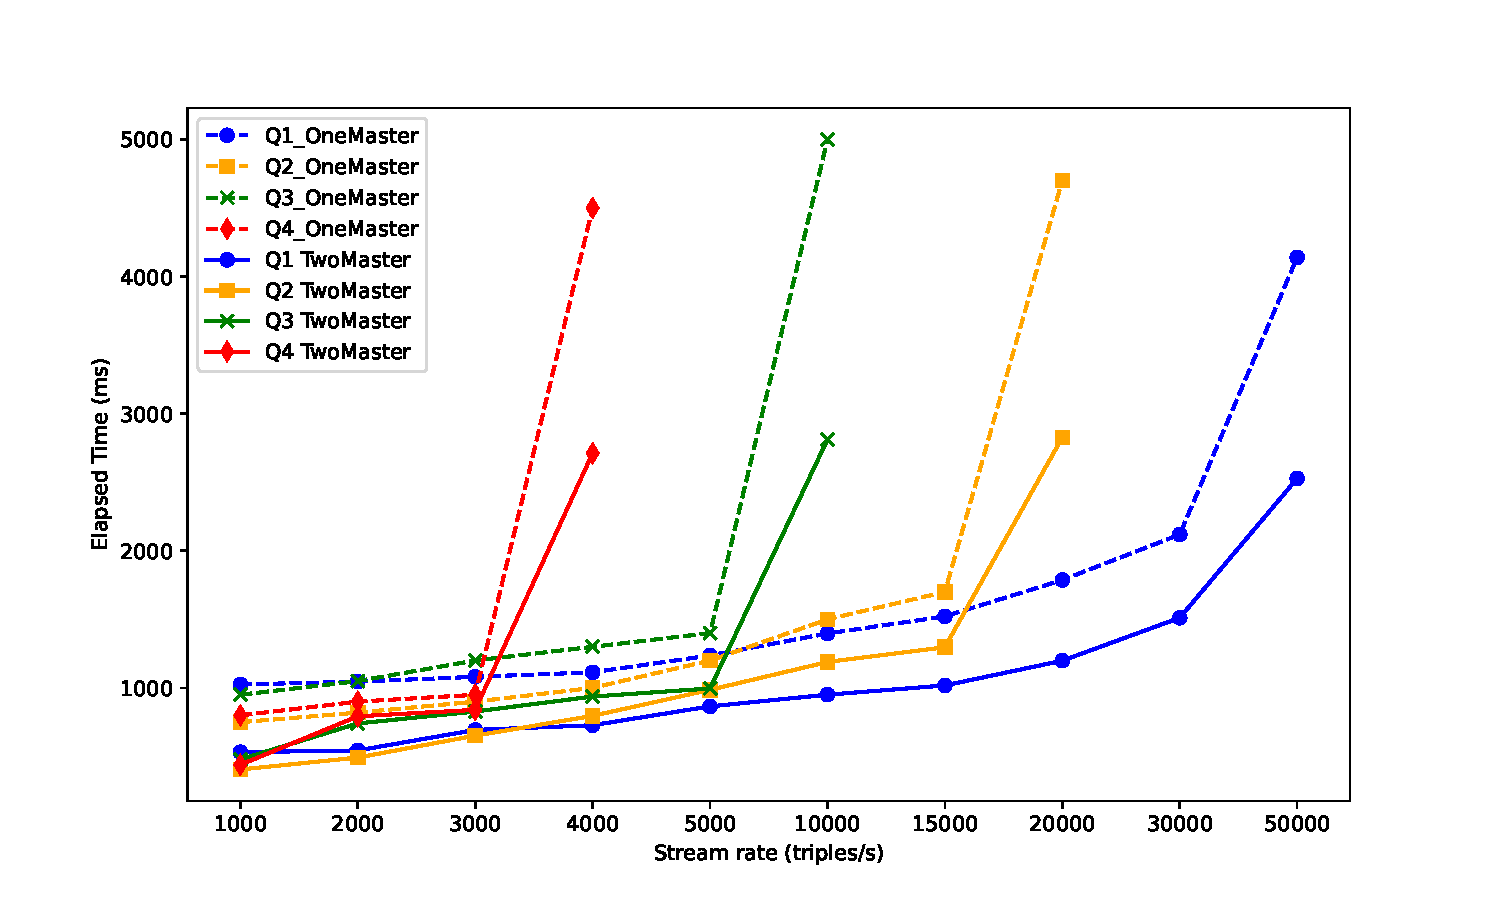
\includegraphics[width=\columnwidth]{result_TwoMaster_OneMaster.pdf}
  \caption{Object refinement performance: independent query execution time for different master nodes}
  \label{fig:resultTwoMasterOneMaster}
\end{figure}

\begin{algorithm}[t]
  \caption{Process Query}\label{alg:conceptQuery}
  \begin{algorithmic}[1]
  
  \Procedure{ProcessQuery}{$query$}
    \While {$True$}
        \State $Concepts, Locations \gets ExtractConceptsLocations(query)$
        \State $node \gets findNode(Concepts, Locations)$
  
        \If {$node$ exists}
            \State ListenOnNode($node$)
            \State $result \gets Execute(query)$
            \State \Return $result$
        \Else
            \State $node \gets SelectWorkerNode()$
            \State $Entity, Range, hasAddition, ConceptNew,$
            \Statex \hspace{1em} $filterParam, filterConstraints, hasGroup,$
            \Statex \hspace{1em} $hasHaving, hasOrder \gets$
            \Statex \hspace{1em} GetParameterFromConceptOnto(Concepts)
            \State $NewQuery \gets ConstructQuery(Concepts, Locations,$
            \Statex \hspace{1em} $Entity, Range, hasAddition, ConceptNew,$
            \Statex \hspace{1em} $filterParam, filterConstraints,$
            \Statex \hspace{1em} $hasGroup, hasHaving, hasOrder)$
  
            \State UpdateNodePlatform(Concepts, Locations, node)
            \State SendQueryToNode($NewQuery, node$)
        \EndIf
    \EndWhile
  \EndProcedure
  
  \end{algorithmic}
\end{algorithm}







\begin{algorithm}[t]
  \caption{Construct Query}\label{alg:constructquery}
  \begin{algorithmic}[1]
  \Procedure{ConstructQuery}{$Concept, Location, Entity, Range,$
  $hasAddition, ConceptNew, filterParam,$
  $filterConstraints, hasGroup, hasHaving, hasOrder$}
  
  \State $query \gets$
  \Statex \hspace{2em} \texttt{CONSTRUCT \{$?l$ concept:\{$Concept$\} $?a$\}} 
  \Statex \hspace{2em} \texttt{FROM STREAM \{$Location$\} [RANGE \{$Range$\}]}
  \Statex \hspace{2em} \texttt{WHERE \{ \{$Entity$\} concept:\{$ConceptNew$\} \{$filterParam$\},}
  \Statex \hspace{2em} \texttt{\{$Entity$\} \{$hasAddition$\},}
  \Statex \hspace{4em} \texttt{FILTER (\{$filterConstraints$\})}
  \Statex \hspace{2em} \texttt{\}}
  \Statex \hspace{2em} \texttt{GROUP BY \{$hasGroup$\}}
  \Statex \hspace{2em} \texttt{HAVING \{$hasHaving$\}}
  \Statex \hspace{2em} \texttt{ORDER BY \{$hasOrder$\}}
  
  \EndProcedure
  \end{algorithmic}
  \end{algorithm}

%\twocolumn % Switch to one column
\section{Evaluation}

The DiSIF framework is implemented in the Java programming environment. The codes written for the semantic nodes are independent of the communication layer, allowing the use of various communication channels such as MQTT or WebSocket. The communication channel in the DiSIF framework is based on Apache Kafka. In the system implementation, we utilize C-SPARQL as the RDF stream processor (RSP). 
Next, we explore the evaluation of the centralized JDL approach and the distributed JDL approach.

As mentioned, in the centralized JDL fusion model, generating the desired outputs requires collecting all the necessary data in a central node, where queries and corresponding components are executed on these aggregated data to produce the outputs. In contrast, in the distributed JDL approach, there is no need to send all data to a central node. Instead, by distributing query processing, only the query execution results are sent to other nodes.



Comparison of centralized and distributed JDL approaches can be analyzed from five perspectives:

\begin{itemize}
    \item \textbf{Network Load} 


In the centralized approach, since all RDF data needs to be sent to the master node, the network load increases significantly, leading to a decrease in network efficiency. The volume of raw data sent over the network to the master node is much larger than the processed data. In terms of the amount of data transmitted and data transfer speed, the approach of sending processed data is preferable to sending raw data. This makes the distributed JDL approach more network-efficient than the centralized JDL approach.
    
    \item \textbf{Execution Time of Dependent Queries}


In the JDL model, the situation refinement component, requiring the use of outputs from the object refinement component, executes dependent queries for output generation.
As subqueries need to be executed first to provide the necessary input for dependent queries, the time to produce outputs for dependent queries increases. In the centralized approach, both subqueries and dependent queries are executed on a single node, while in the distributed JDL approach, subqueries are executed on worker nodes, and dependent queries are executed on the master node. Consequently, the execution time of dependent queries is reduced, making it more efficient compared to the centralized approach.
    
    \item \textbf{Execution Time of Independent Queries}


    In the JDL model, the object refinement component includes independent queries that operate on raw data and do not require the execution of other queries as prerequisites. In the distributed approach, these queries can be executed across different nodes, enhancing the execution time of independent queries compared to the centralized scenario.
    
    \item \textbf{Memory Consumption}


 In the centralized JDL model, the execution of independent and dependent queries on a single node can significantly impact their memory consumption. On the other hand, the distributed JDL approach has demonstrated better memory management compared to the centralized approach.
    
    \item \textbf{Data Security}


 One of the challenges of the centralized JDL method is that all data must be sent from other nodes to the master node, posing potential security issues. In many applications, data from nodes cannot be transferred to the master node due to security concerns and must be used locally. Therefore, the distributed JDL approach is introduced to overcome this challenge. In this approach, there is no need to send raw data from other nodes to the central node, and data processing can be performed locally on local data, with the results sent to the master node. Thus, the security issue related to data transfer is mitigated in this distributed approach.
\end{itemize}



In this section, we analyze the centralized and distributed JDL approaches in terms of executing various JDL components.
To evaluate the object refinement component in the edge layer and the situation refinement component in the fog layer, we analyze the executing of independent and dependent queries, respectively, in both centralized and distributed scenarios.


%\onecolumn % Switch to one column
\begin{algorithm}[t]
  \caption{Query Response in masterNode}
  \label{alg:QueryresponsemasterNode}
  \begin{algorithmic}[1]
      \setstretch{1} % Adjust the spacing factor as needed
      \State \textbf{Input:} User query 
      \State \textbf{Output:} Query response

      \State Receive user query by UCI and send to RSP component
      \If{SPARQL query}
          \State Execute query on database and get results.
      \ElsIf{C-SPARQL query}
          \If{Query's concepts exist in NodePlatform}
              \If{Query's locations exist in NodePlatform}
                  \State Split the query by locations into independent sub-queries.
                  \State Assign each sub-query to corresponding node registered in NodePlatform.
                  \State Aggregate results of sub-queries. 
              \Else
                  \State Expand each query stream/location with its 
                  sub-streams/sub-locations according to the cityOnto.
                  \State Repeat the steps from line 6.
              \EndIf
          \Else
              \State Create a new query for generating the desired concept 
              based on Algorithm \ref{alg:conceptQuery} using the conceptOntology.
          \EndIf
      \EndIf
  \end{algorithmic}
\end{algorithm}





\subsection{Object refinement performance in the Edge layer}


The data in this layer consists of sensor data (level one), and the queries processed at this level are classified as level one or independent queries. 
Consequently, the fusion operation occurs at the sensor level, referred to as sensor/data fusion. Subsequently, the performance of the DiSIF framework is analyzed in terms of the execution time of level one/independent queries in the edge layer.

\subsubsection{Centralized and Distributed approaches}
In these experiments, we analyze the time required to execute queries Q1, Q2, Q3, and Q4
 (shown in \ref{sec:AppendixQueries}) from the perspective of the stream rate.


%\begin{figure*}
%  \centering
%  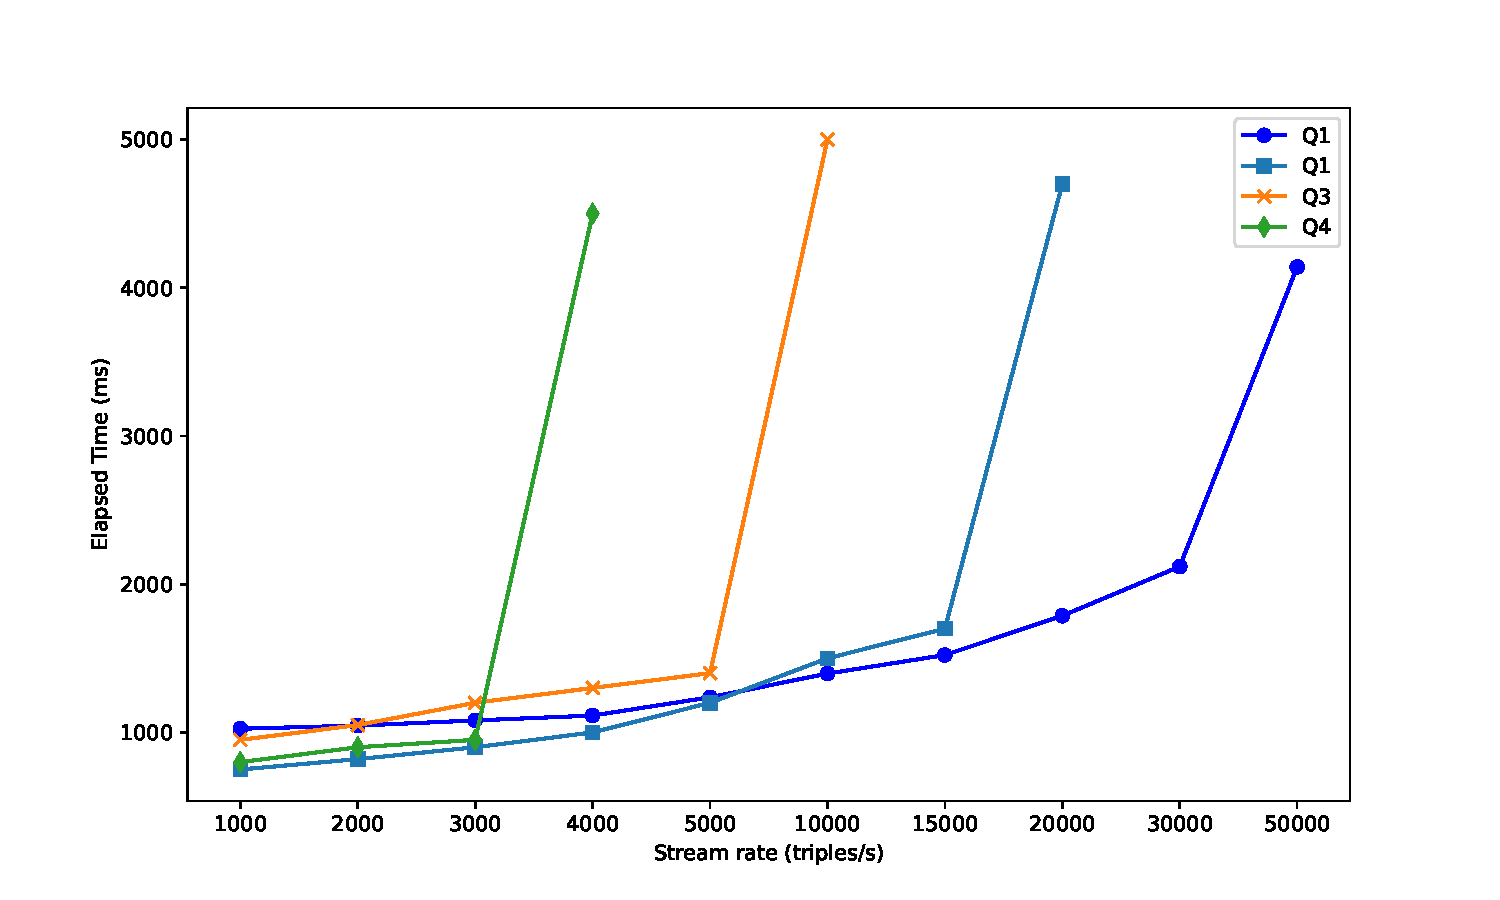
\includegraphics[width=0.8\textwidth]{C:/Users/Administrator/Desktop/Thesis_latex_Final/result_OneMaster.pdf}
%  \caption{Query execution time for different stream rates}
%  \label{fig:resultOneMaster}
%\end{figure*}


in Figure \ref{fig:resultTwoMasterOneMaster} , the results of executing various queries in the centralized scenario, where only one edge master node exists and for distributed approach with two edge master nodes,
 are presented. In this case, the execution time of queries is analyzed for different stream rates.
 As observed, for query Q1, the execution time experiences a sudden increase at a stream rate of 30000 triples/s.
 Similarly, query Q2 shows a sudden increase at a stream rate of 15000 triples/s, Q3 at 5000 triples/s, and finally, Q4 at 3000 triples/s. 

The reason for this phenomenon is that, in C-SPARQL, as the complexity of a query increases, its ability to manage high stream rates decreases.
 When the stream rate exceeds the response capacity of C-SPARQL, the execution time of the query experiences a sudden increase.
For this reason, in cases where a query is broken down into independent subqueries and multiple edge master nodes are available for query execution, 
each subquery can be executed on a separate edge master node and the results are then combined, enabling the main query to be executed in parallel. 
Consequently, the execution time of queries significantly improves in distributed approach.






As depicted in Figure \ref{fig:resultTwoMasterOneMaster}, the execution time for different stream rates is approximately halved. The reason for this slight increase in the execution time is that a short period is spent aggregating the results from these two nodes. Therefore, in comparison to the centralized approach for executing independent queries, this distributed scenario exhibits lower execution times.


\subsection{Situation refinement performance in the Fog layer}

In this section, we evaluate the performance of the distributed JDL fusion model in comparison to the centralized JDL, focusing specifically on the situation refinement component and the execution of dependent queries.
The scenarios of congestion detection and traffic discovery are examined as two dependent scenarios or queries.

The data flowing between nodes in the fog layer is categorized as level two. In other words, this data consists of processed information from the lower edge layer, rather than raw sensor data.  Consequently, the fusion operation at this level involves information fusion, and the queries executed by fog layer managers are focused on concepts that require prepared input data for their execution.

In the centralized JDL approach, obtaining the results of the situation refinement component requires the outputs of the object refinement component to be initially placed on the BUS associated with the centralized JDL. Consequently, object refinement and situation refinement queries are interdependent and must be executed in a sequential manner.


In the following, we evaluate the two components, object refinement and situation refinement, for the scenarios of congestion detection and traffic discovery, respectively.



\section*{Traffic Discovery Scenario}

For traffic discovery, the query \(Q_m\) is defined in \ref{sec:AppendixQueries} .

As indicated by query \(Q_m\), congestion event messages are received within 3-second windows. 
In this query, \texttt{?s} represents the streets (as locations) where congestion has occurred. If a street experiences congestion more than three times within a 3-second window, it is classified as congested. 
To execute this query, congestion event messages must be generated, which are produced by worker nodes within the same fog layer. 



\section*{Congestion Detection Scenario}

To evaluate the performance of both centralized and distributed JDL approaches for congestion detection,
 we employ various queries with diverse complexities as detailed in the \ref{sec:AppendixQueries} 
 as Queries \(Q_1\),\(Q_2\),\(Q_3\),\(Q_4\).

\textbf{Query \(Q_1\)}

In this query, the output highlights regions where the speed of at least one vehicle is below 50 km/h, indicating congestion. This query is specifically designed to detect congestion and generate congestion event messages based on the location, speed, and timestamp of vehicles within the specified stream.

\textbf{Query \(Q_2\)}

Continuing with the congestion detection scenario, Query \(Q_2\) identifies regions where at least three vehicles have speeds below 50 km/h, indicating congestion. The results are then sorted in ascending order based on location. This query establishes a more specific criterion for detecting congestion by taking into account both the speed condition and the minimum number of vehicles present in a given area.

\textbf{Query \(Q_3\)}

This query, similar to Query \(Q_2\), congestion is detected in areas with "2," "3," or "1" in their titles (?location). Additionally, the average speed of vehicles is returned as output for each location. This query offers insights into both congestion detection and the average speed of vehicles in specific locations.

\textbf{Query \(Q_4\)}

This operates similarly to Query \(Q_3\), with the difference that it uses UNION to also analyze areas whose title includes "4". This allows the query to provide insights into congestion detection and average speed in regions containing "2", "3", "1", or "4".


We evaluate the situation refinement component from three perspectives: query execution time, memory consumption,
 and network load. Each of these aspects will be examined in detail. Assume that executing the user query \(Q_m\) requires the execution of \(n\) prerequisite queries \(Q_i\).

\subsubsection{Query execution time}


In this section, we first express the formula for calculating the execution time of query $Q_m$ in centralized and distributed approaches as follows.


\begin{itemize}

\item Centralized approach


In the centralized approach, all raw data must be transferred from the worker nodes to the master node before executing query \( Q_m \) on the master node.

\begin{equation}
T_c = T_{\text{data transfer}} + \sum_{i \in N} T_{Q_i} + T_{Q_m}
\end{equation}

where \( T_{\text{data transfer}} \) is the time required to transfer raw data from all worker nodes to the master node, \( T_{Q_i} \) is the time taken to execute query \( Q_i \) on the master node, and \( T_{Q_m} \) is the time required to execute query \( Q_m \) on the master node.

\item Distributed approach

In the distributed approach, each query is executed on its respective worker node, and the results are transferred to the master node, where the query \( Q_m \) is executed. The execution time in the distributed approach is as follows:

\begin{equation}
T_d = \max(T_{Q_i}) + T_{\text{result transfer}} + T_{Q_m}
\end{equation}

As can be observed from the equations, in the centralized approach, the execution time increases linearly with the increase in the number of queries \( Q_i \). This is due to the sequential processing. In the distributed approach, the queries are processed in parallel, which reduces the execution time to the maximum time required to execute any of the \( Q_i \) queries. Therefore, for a large number of requests \( N \), the distributed approach significantly reduces the execution time compared to the centralized approach due to parallel execution.


% \begin{figure}[htb] % Inline figure with appropriate size
%   \centering
%   \begin{subfigure}{0.48\textwidth} % Use column width for inline placement
%     \centering
%     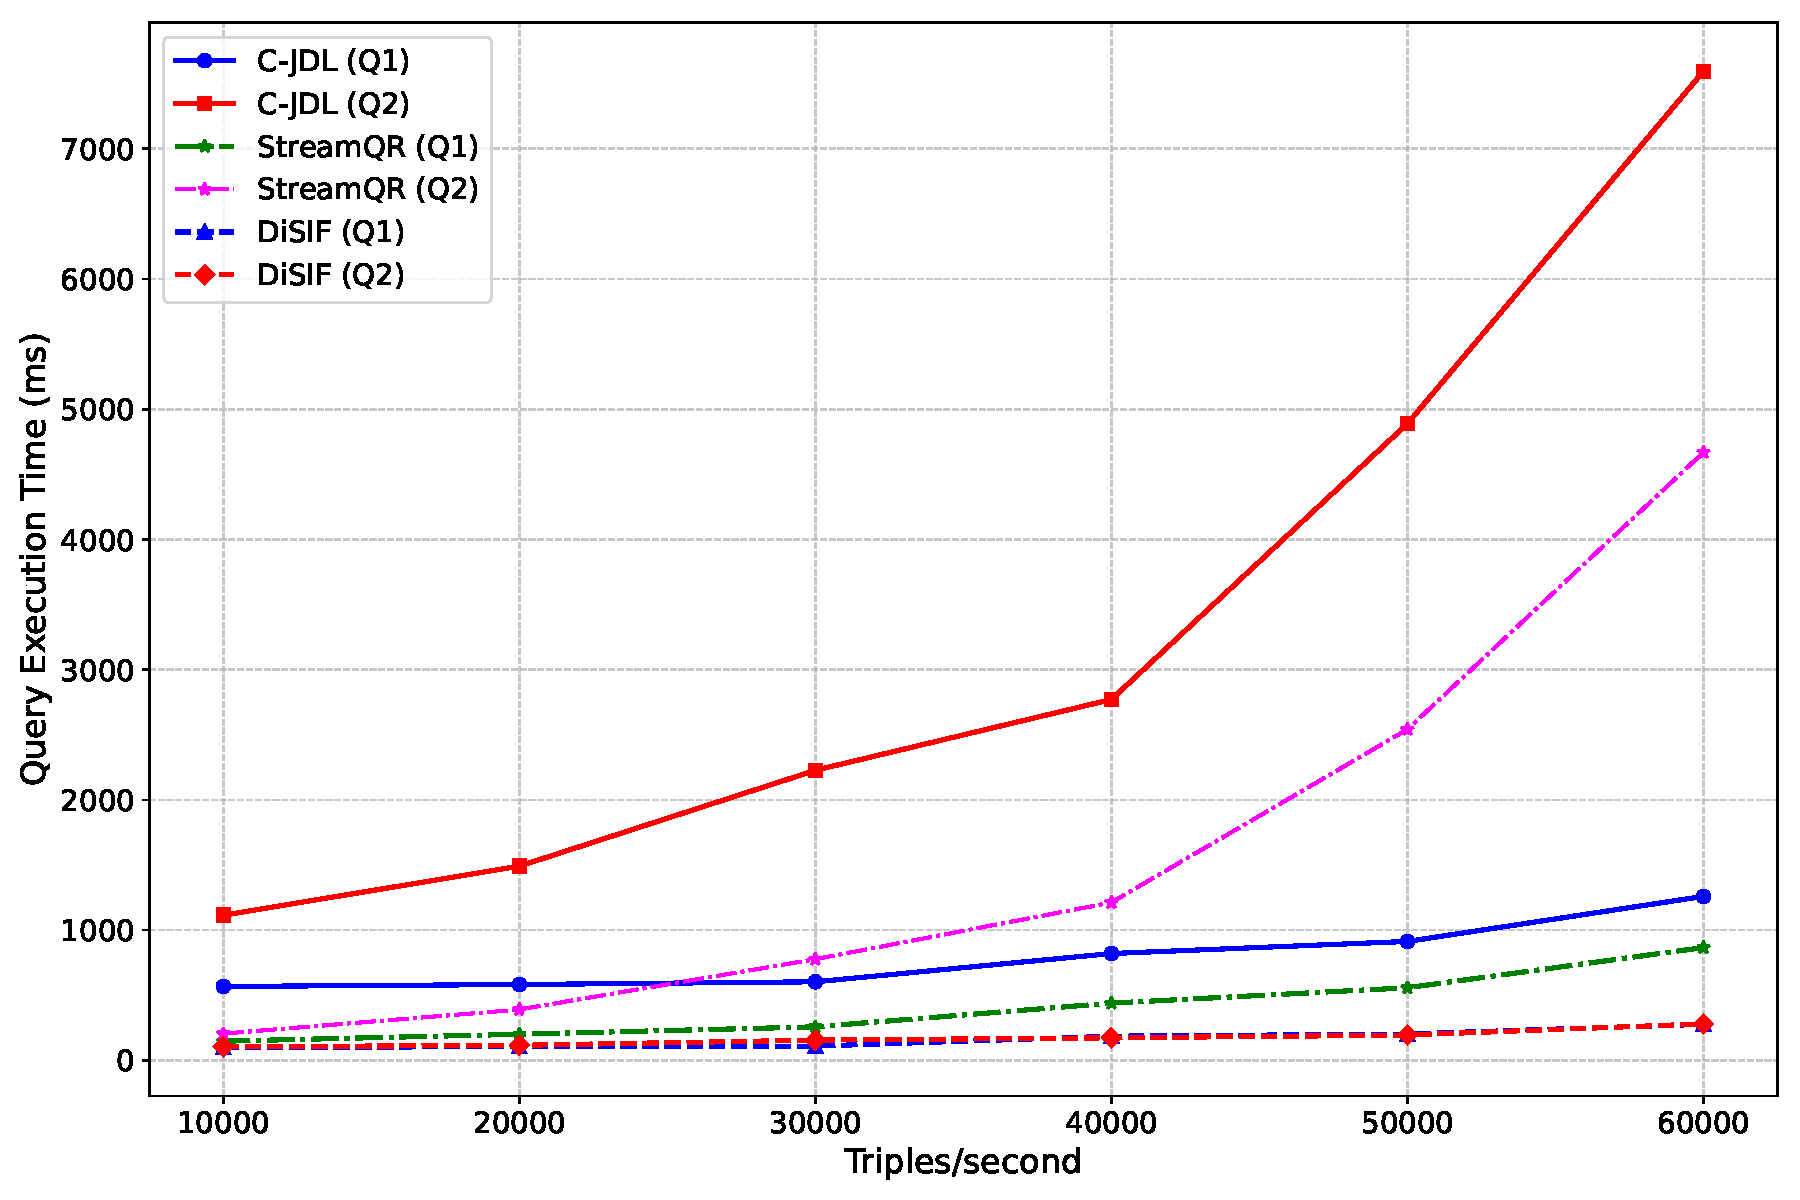
\includegraphics[width=\columnwidth]{Time_execution_Q1Q2_StreamQR_NonLogarithmicAdjustment_LinearScale_Q1Q2.pdf}
%     \subcaption{Comparing Execution Times for Q1 and Q2 in Centralized and Distributed Environments}
%     \label{fig:Timeexperiment1}
%   \end{subfigure}
%   \hfill
%   \begin{subfigure}{0.48\textwidth} % Same size for balance
%     \centering
%     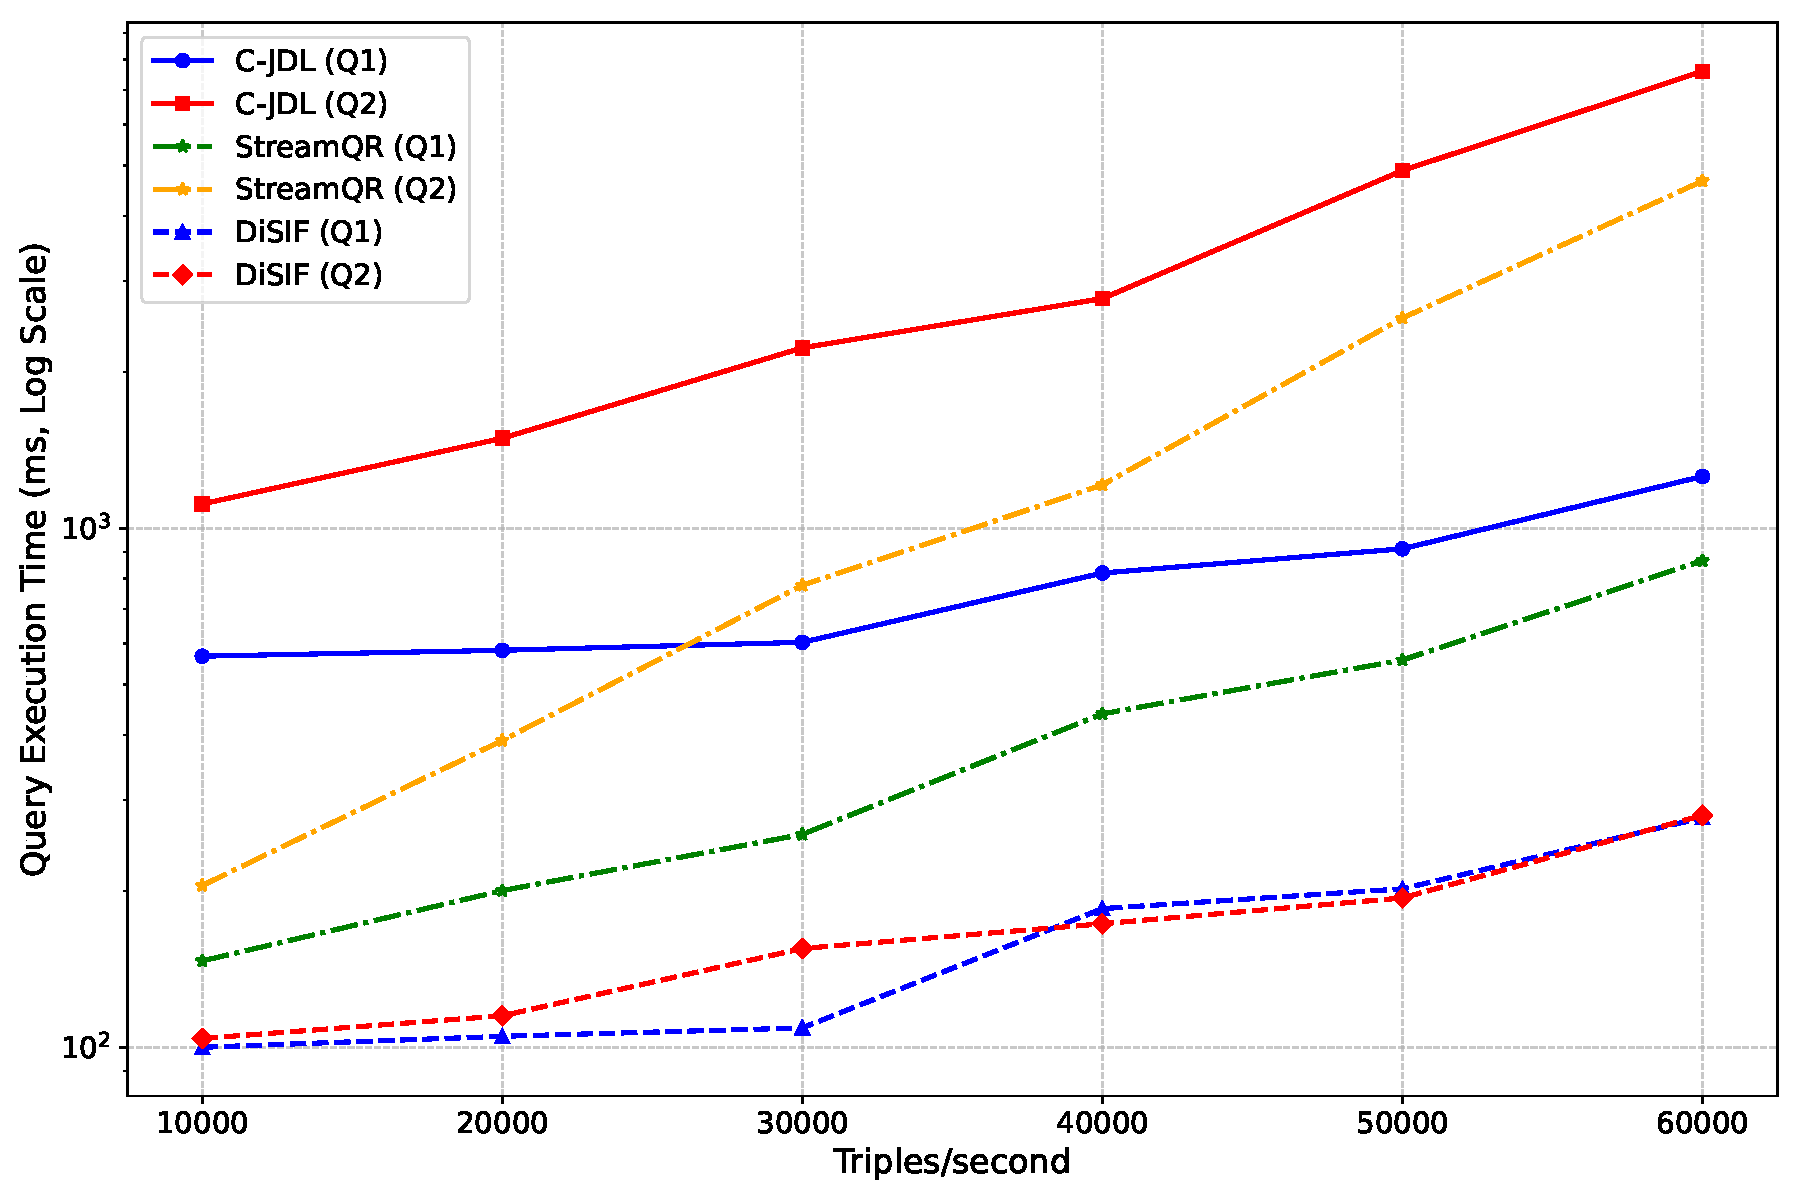
\includegraphics[width=\columnwidth]{Time_execution_Q1Q2_StreamQR_NonLogarithmicAdjustment_LogScale_Q1Q2.pdf}
%     \subcaption{Comparing Logarithmic Execution Times for Q1 and Q2 in Centralized and Distributed Environments}
%     \label{fig:Timeexperiment2}
%   \end{subfigure}

%   \vspace{1cm} % Vertical space between the row of subfigures
%   \begin{subfigure}{0.48\textwidth} % Use column width again for inline placement
%     \centering
%     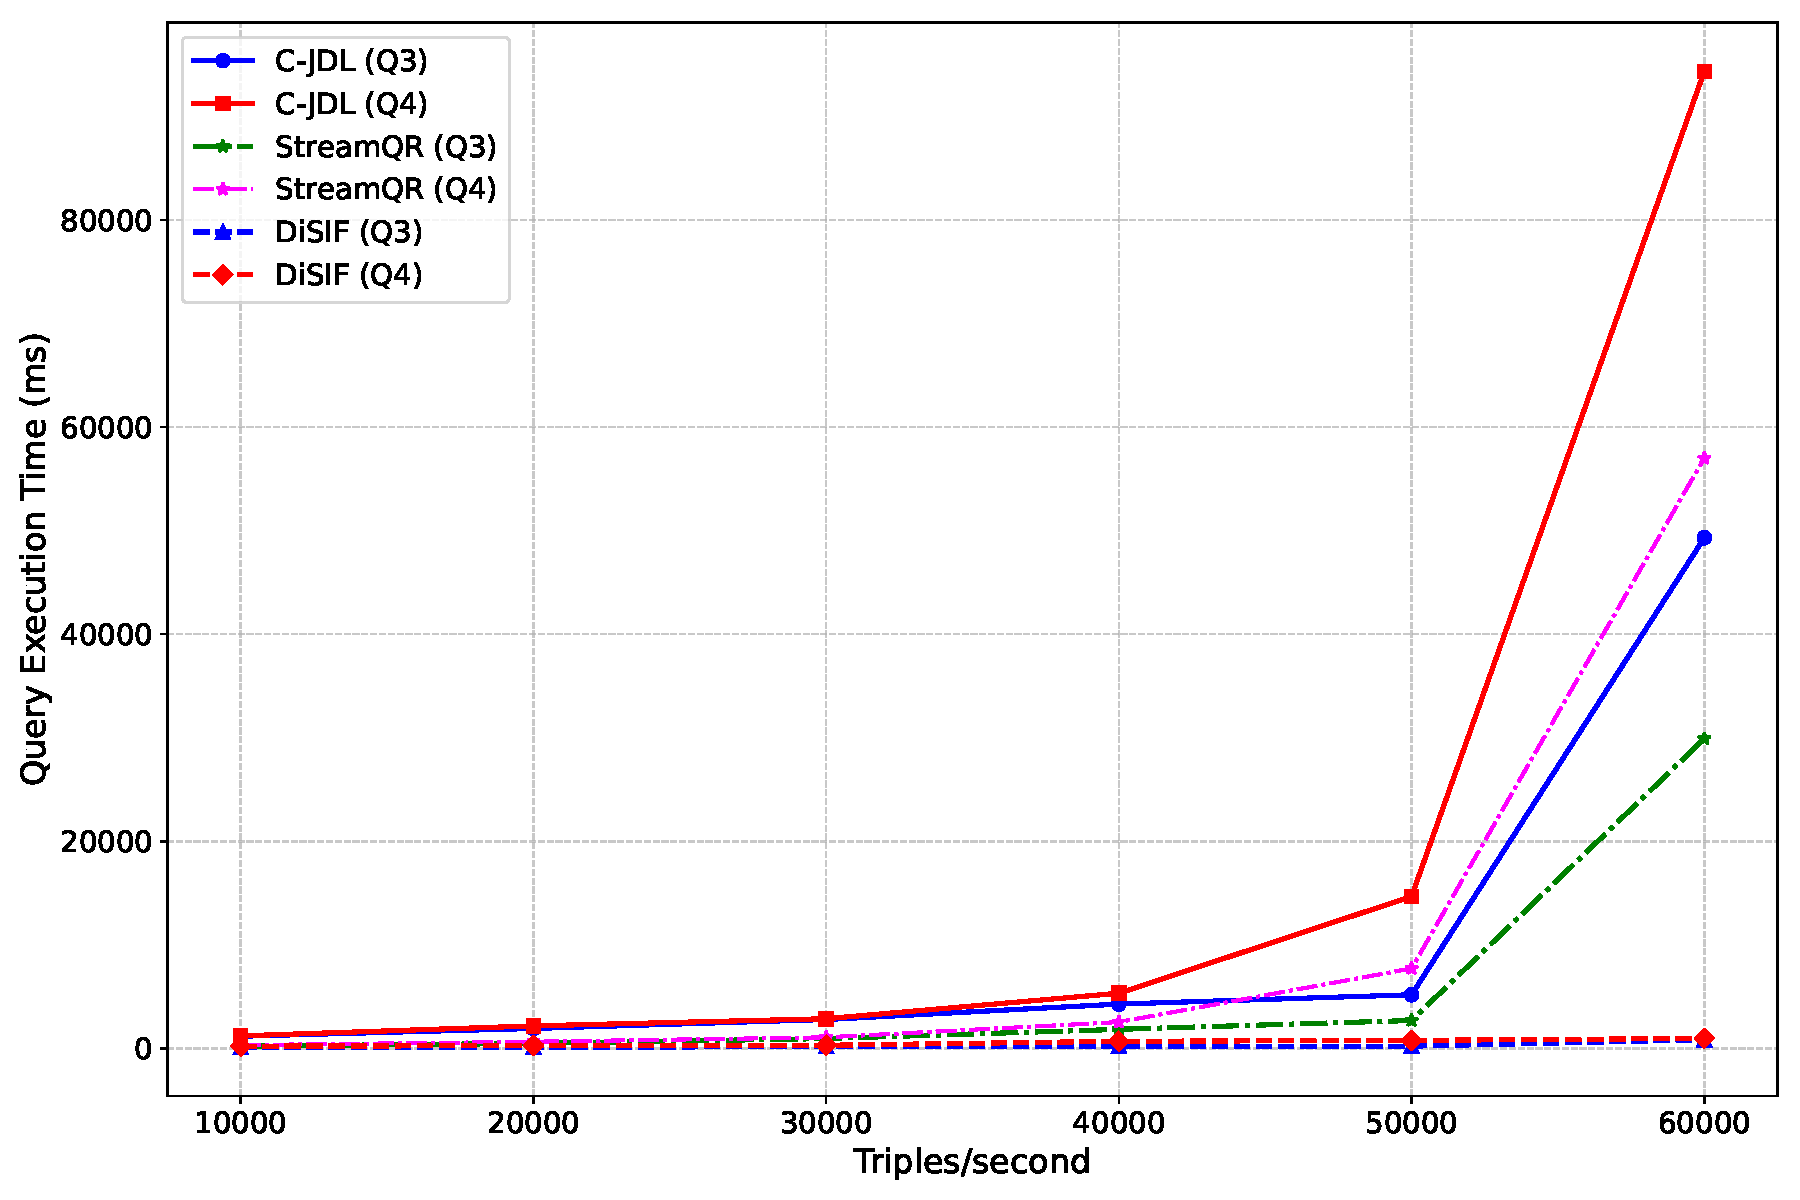
\includegraphics[width=\columnwidth]{Time_execution_Q1Q2_StreamQR_NonLogarithmicAdjustment_LinearScale_Q3Q4.pdf}
%     \subcaption{Comparing Execution Times for Q3 and Q4 in Centralized and Distributed Environments}
%     \label{fig:Timeexperiment3}
%   \end{subfigure}
%   \hfill
%   \begin{subfigure}{0.48\textwidth} % Keep consistency in size
%     \centering
%     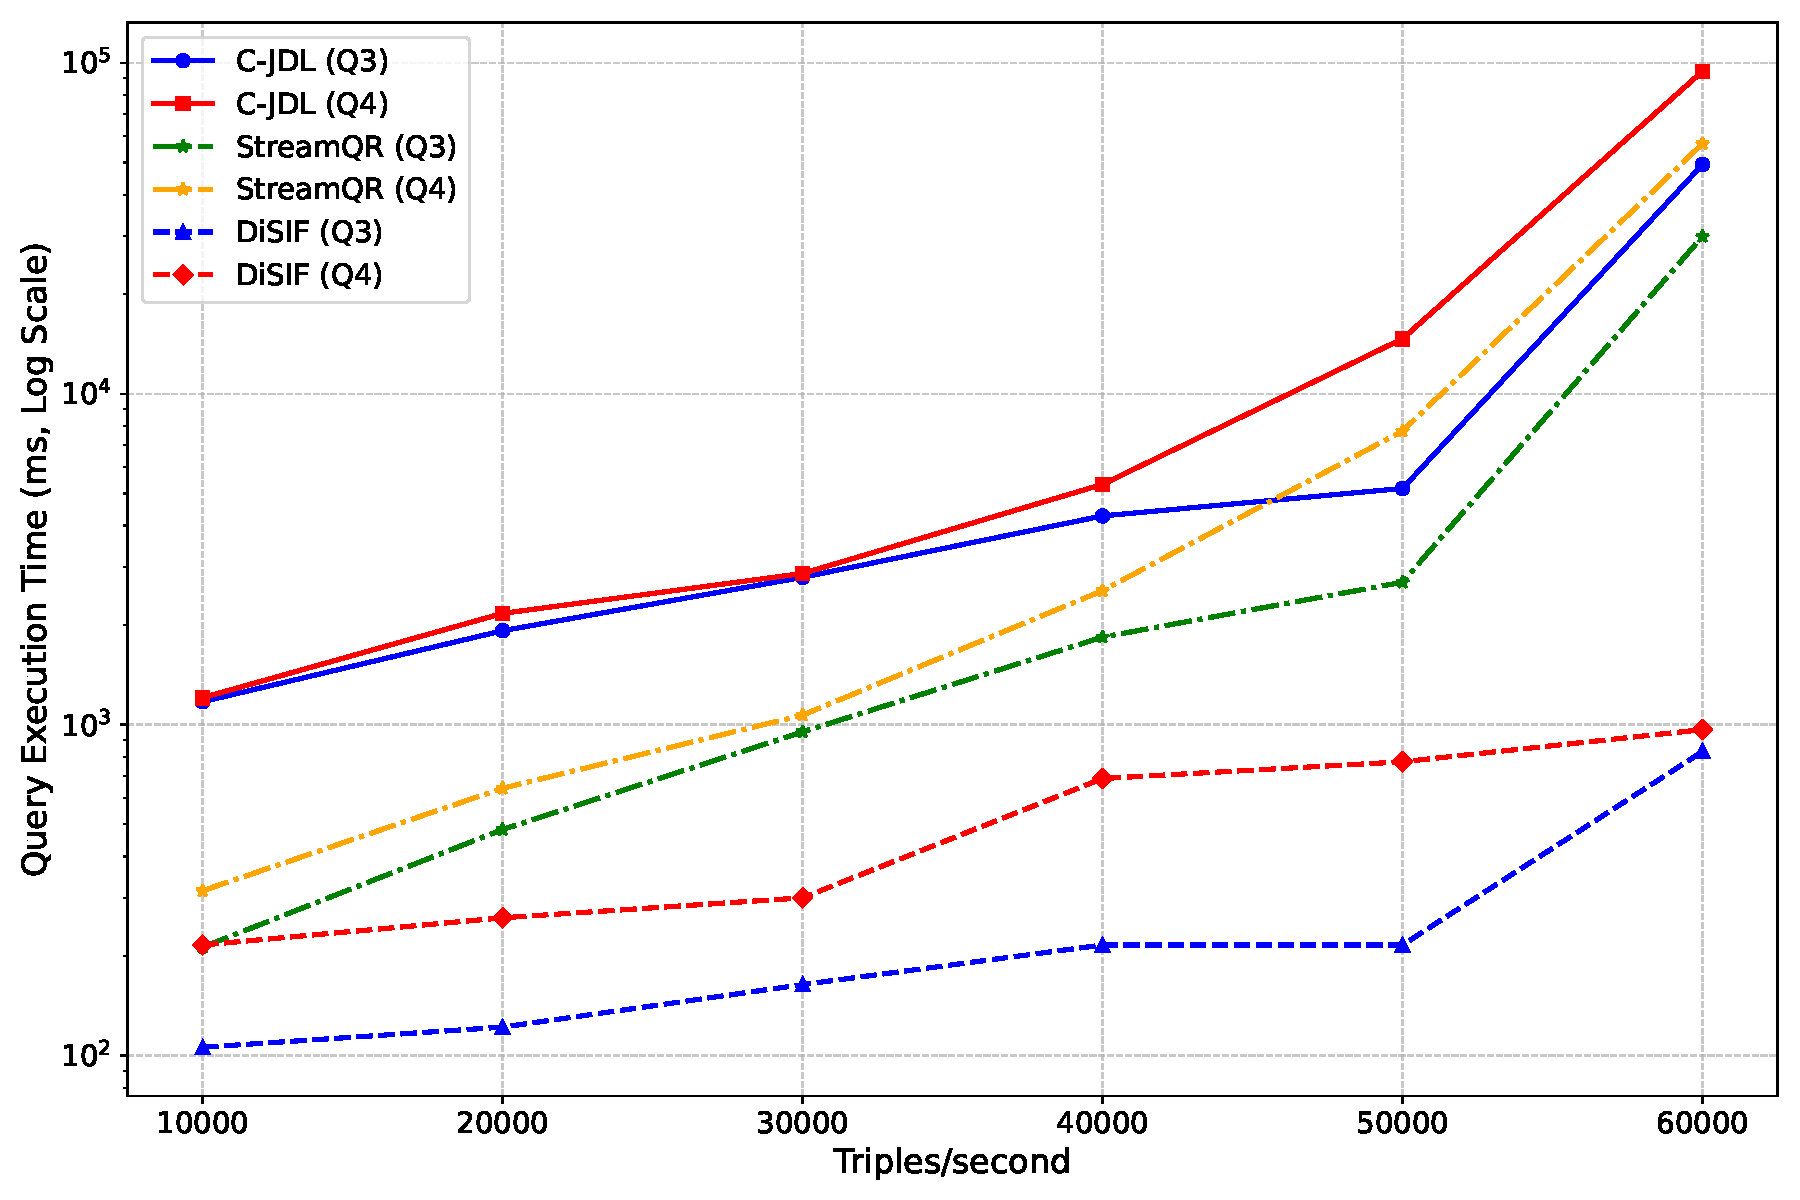
\includegraphics[width=\columnwidth]{Time_execution_Q1Q2_StreamQR_NonLogarithmicAdjustment_LogScale_Q3Q4.pdf}
%     \subcaption{Comparing Logarithmic Execution Times for Q3 and Q4 in Centralized and Distributed Environments}
%     \label{fig:Timeexperiment4}
%   \end{subfigure}
  
%   \caption{Query execution times in Centralized and Distributed Environments}
%   \label{fig:Timeexperiment1234}
% \end{figure}

\begin{figure}[t] % First figure
  \centering
  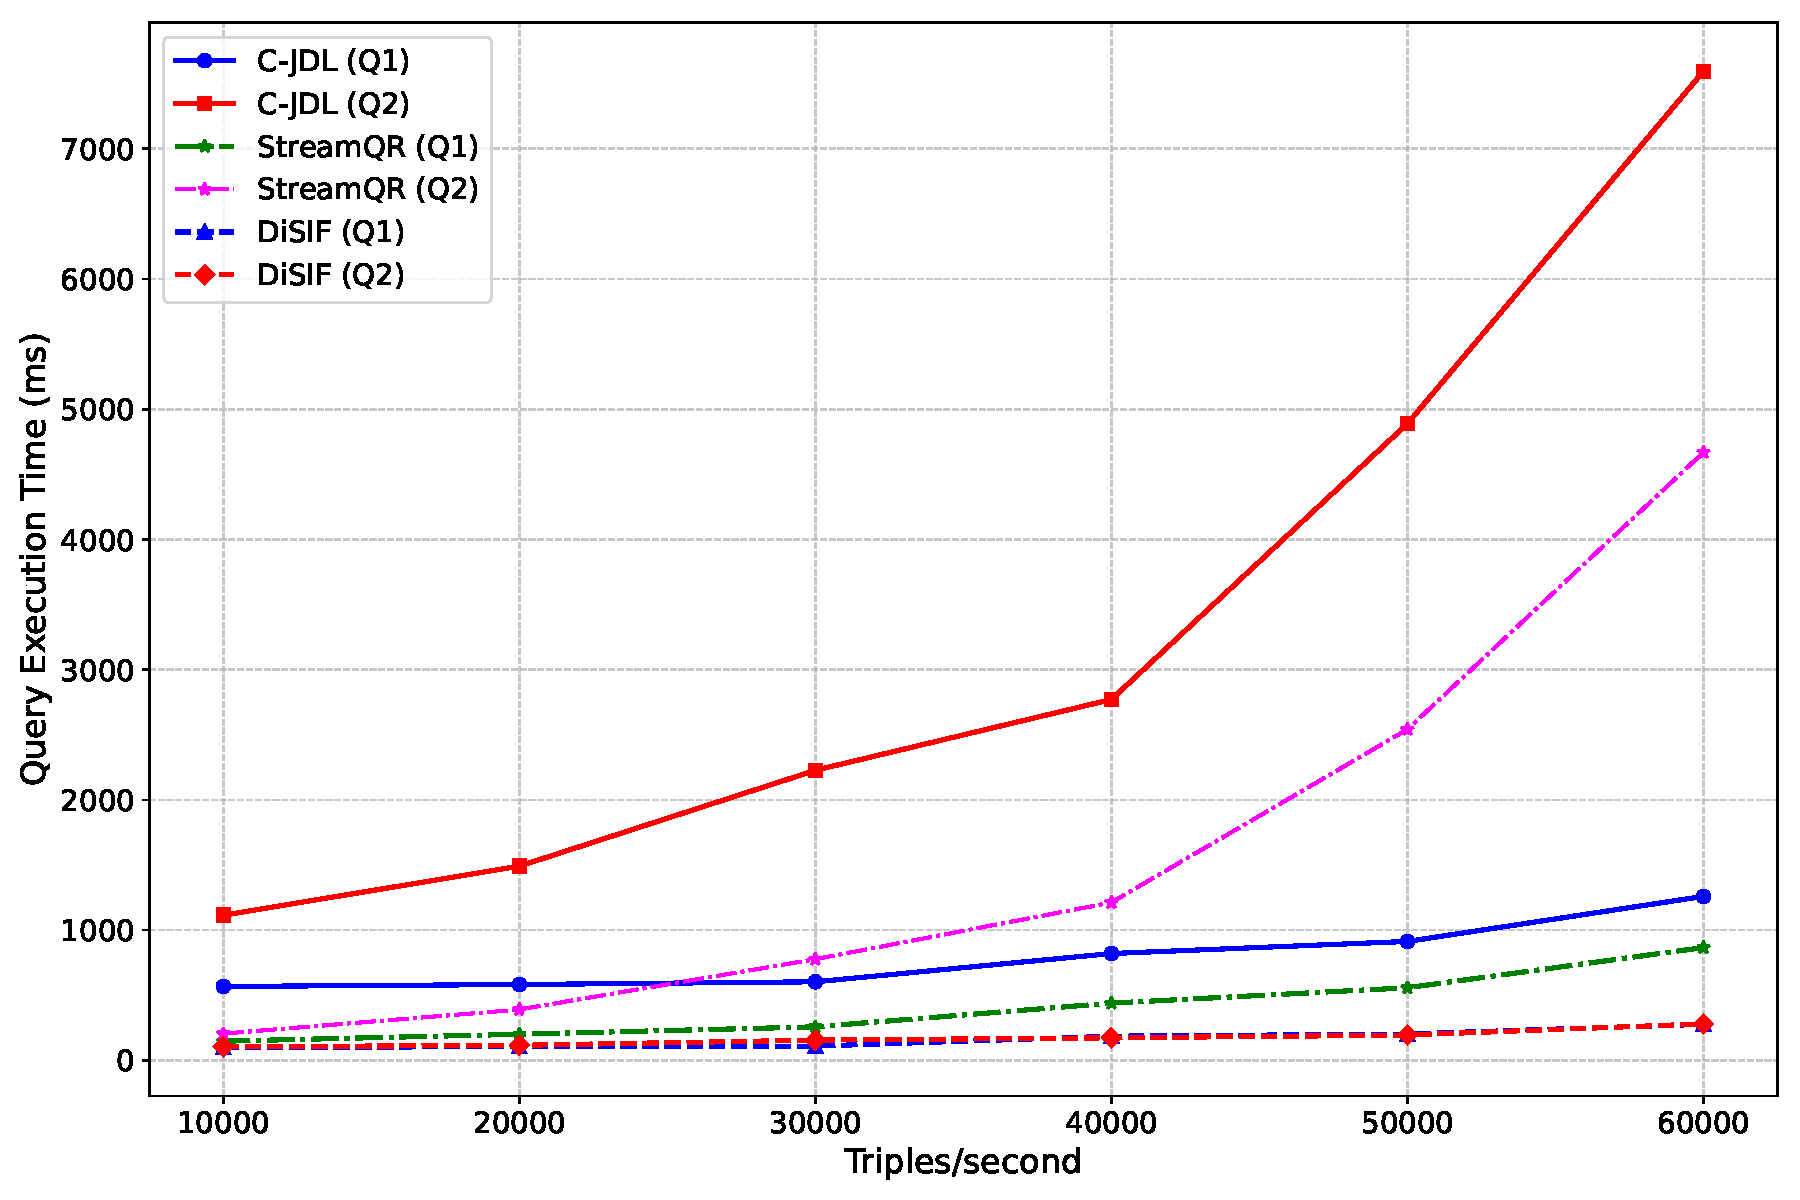
\includegraphics[width=0.8\columnwidth]{Time_execution_Q1Q2_StreamQR_NonLogarithmicAdjustment_LinearScale_Q1Q2.pdf}
  \caption{Comparing Execution Times for Q1 and Q2 in Centralized and Distributed Environments (Linear Scale)}
  \label{fig:Timeexperiment1}
\end{figure}

\begin{figure}[t] % Second figure
  \centering
  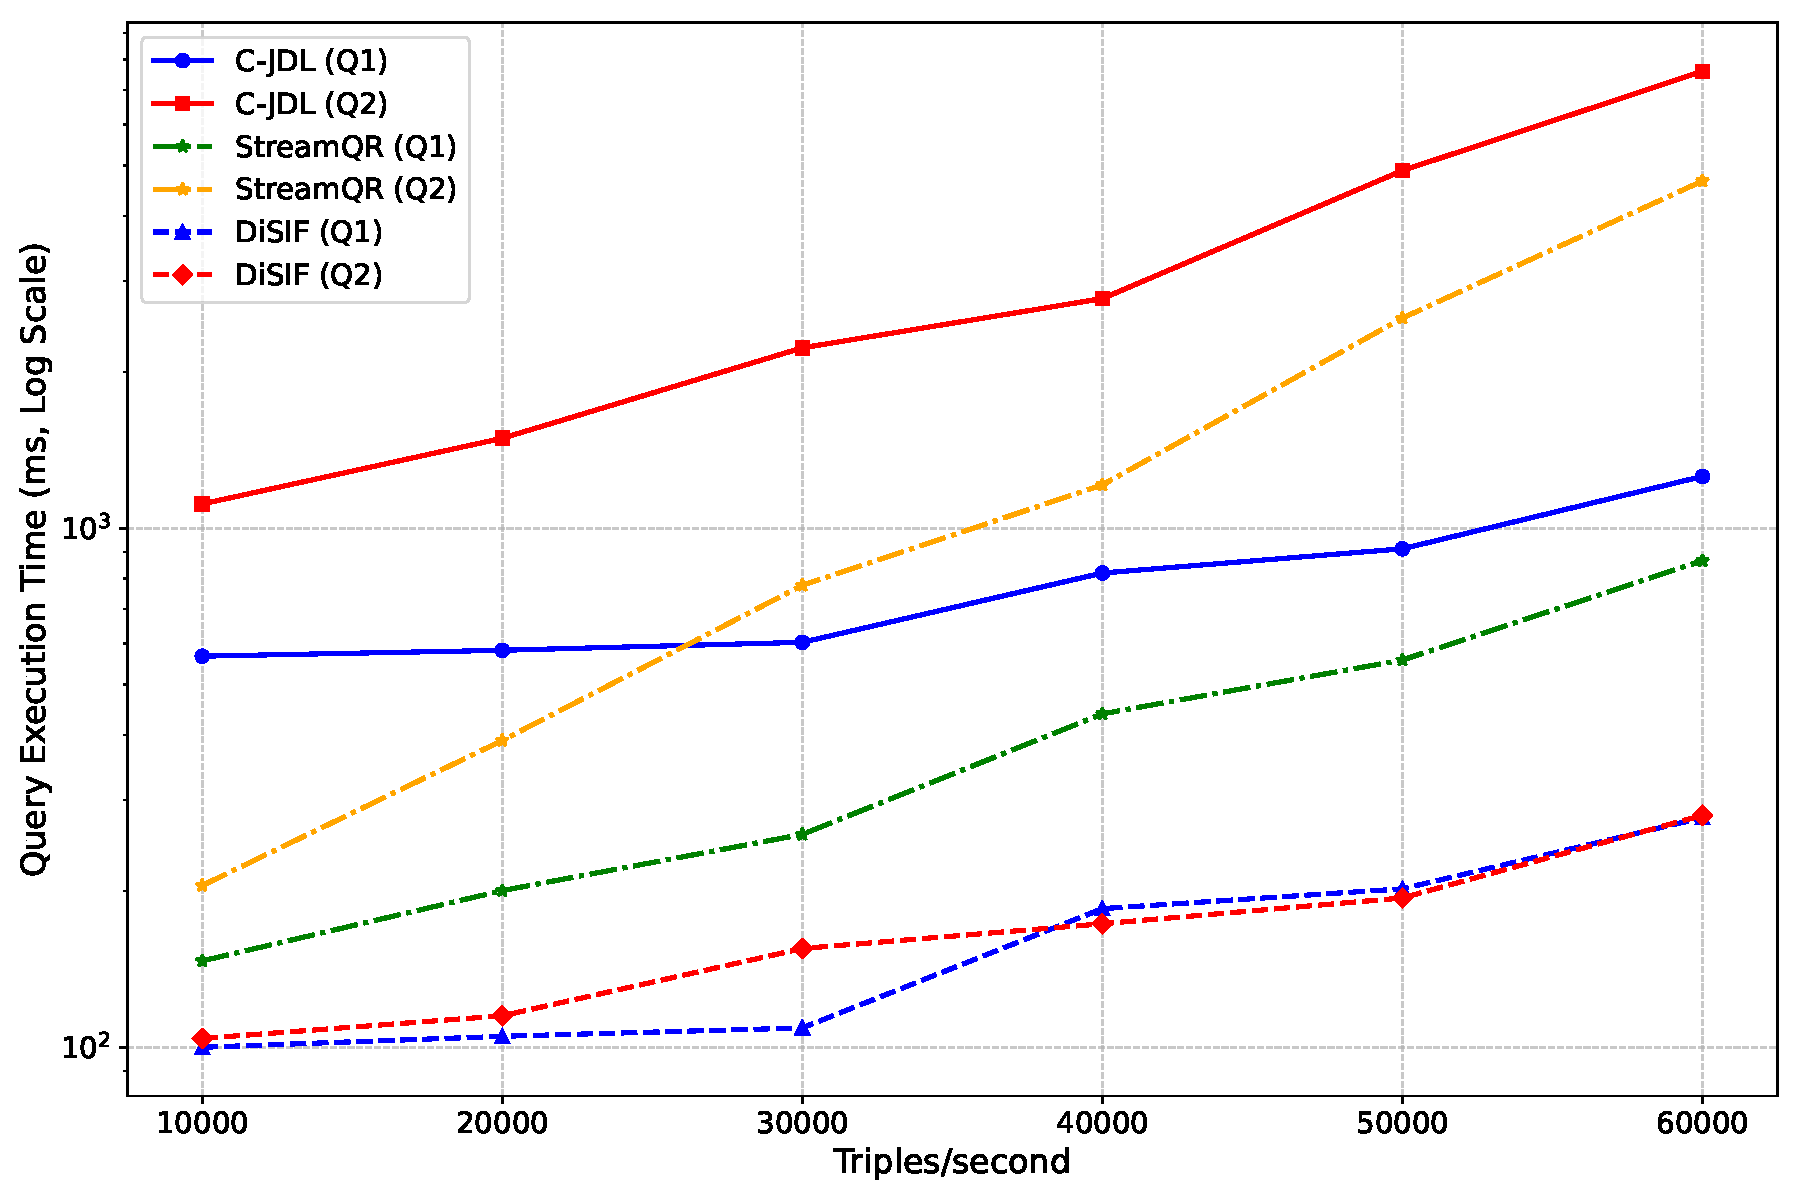
\includegraphics[width=0.8\columnwidth]{Time_execution_Q1Q2_StreamQR_NonLogarithmicAdjustment_LogScale_Q1Q2.pdf}
  \caption{Comparing Logarithmic Execution Times for Q1 and Q2 in Centralized and Distributed Environments}
  \label{fig:Timeexperiment2}
\end{figure}

\begin{figure}[t] % Third figure
  \centering
  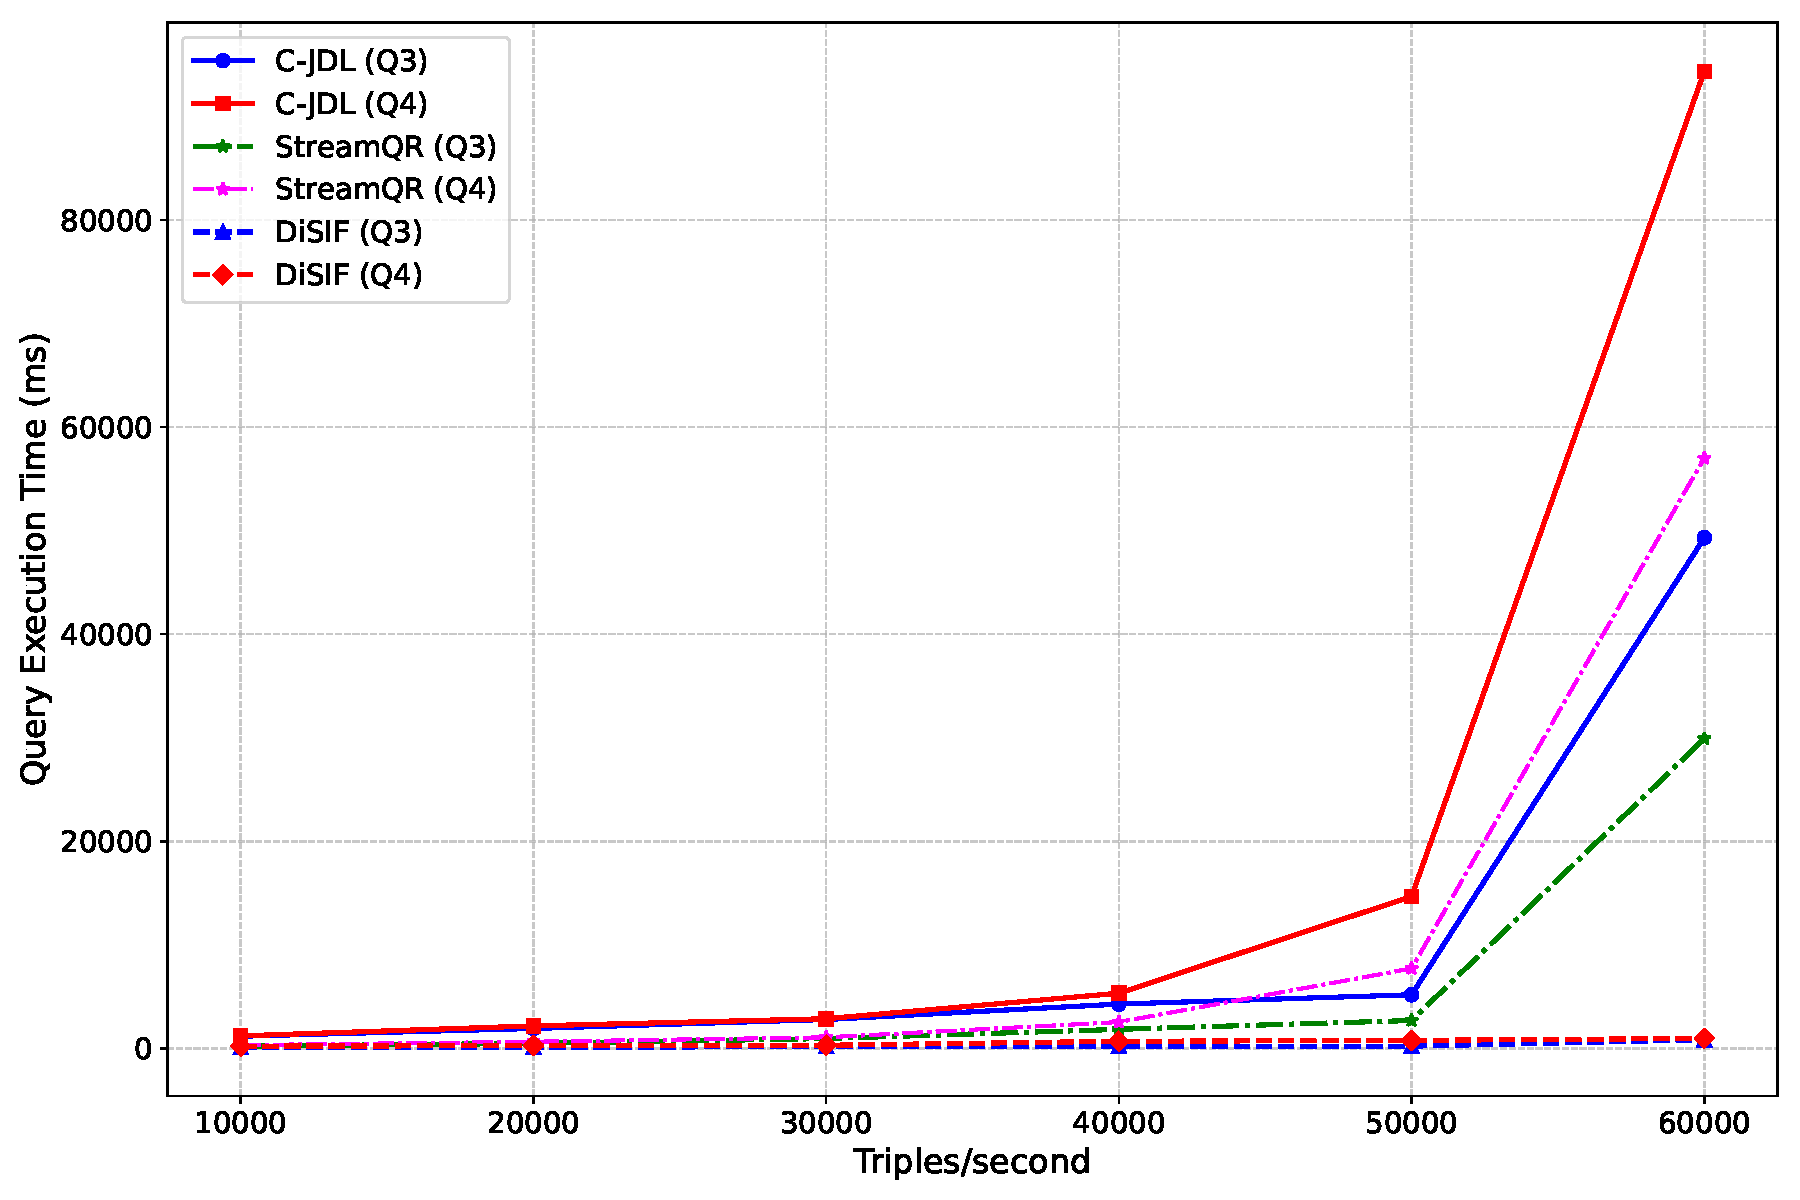
\includegraphics[width=0.8\columnwidth]{Time_execution_Q1Q2_StreamQR_NonLogarithmicAdjustment_LinearScale_Q3Q4.pdf}
  \caption{Comparing Execution Times for Q3 and Q4 in Centralized and Distributed Environments (Linear Scale)}
  \label{fig:Timeexperiment3}
\end{figure}

\begin{figure}[t] % Fourth figure
  \centering
  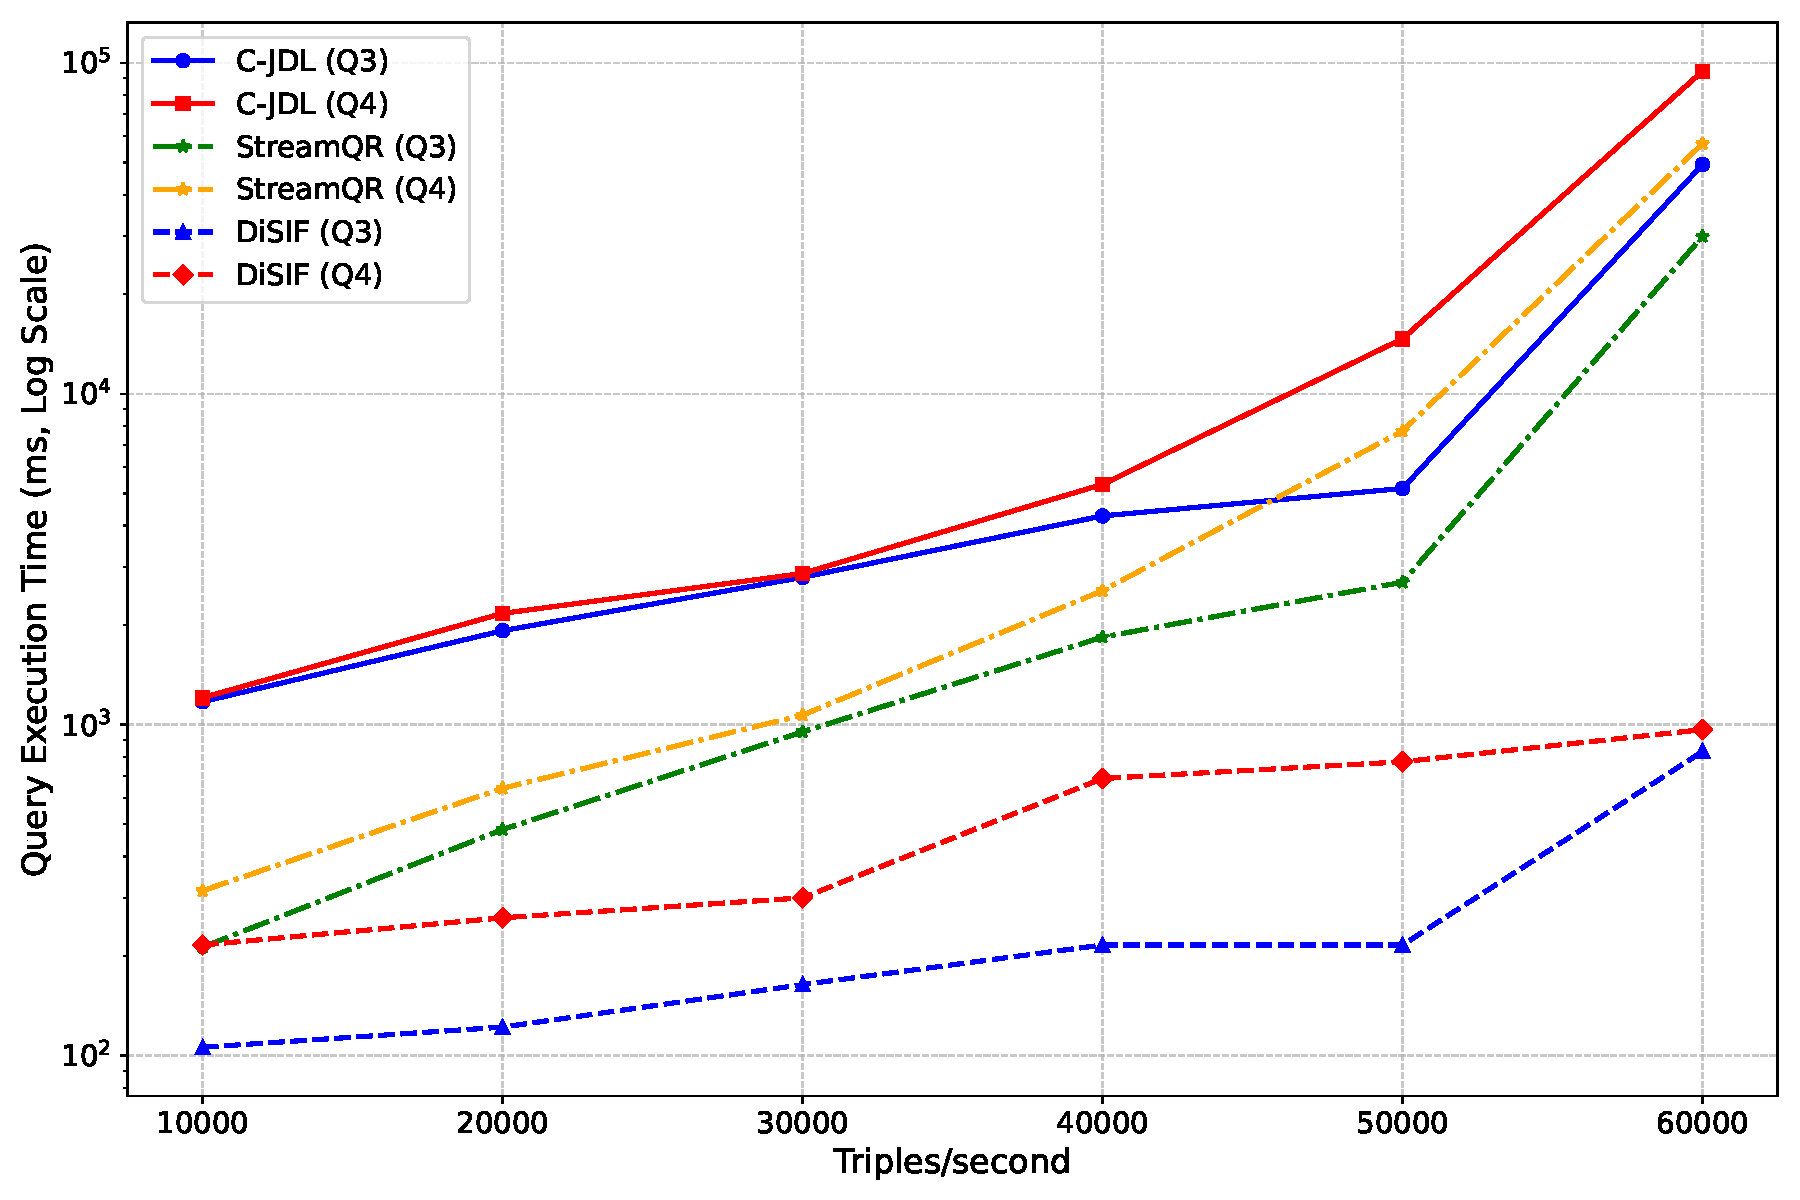
\includegraphics[width=0.8\columnwidth]{Time_execution_Q1Q2_StreamQR_NonLogarithmicAdjustment_LogScale_Q3Q4.pdf}
  \caption{Comparing Logarithmic Execution Times for Q3 and Q4 in Centralized and Distributed Environments}
  \label{fig:Timeexperiment4}
\end{figure}






To analyze the execution time for queries $Q_1$ to $Q_4$ and subsequently query $Q_m$, Figures \ref{fig:Timeexperiment1},\ref{fig:Timeexperiment2},
\ref{fig:Timeexperiment3} and \ref{fig:Timeexperiment4} illustrates the results for various data transmission rates (triples per second).
 This analysis compares both the centralized JDL (C-JDL), StreamQR and DiSIF approaches.


In the C-JDL model, all queries, including $Q_1$, $Q_2$, $Q_3$, or $Q_4$, and $Q_m$, are executed sequentially
 on the master node. For example, during the time analysis of queries $Q_1$ to $Q_4$ and $Q_m$,
  all raw data is sent from the worker nodes to the master node, where the queries are processed.
  This centralized structure leads to exponential growth in query execution time,
   especially for more complex queries (like $Q_3$ and $Q_4$), as the data transmission rate (triples/sec)
    increases. This increase is due to $Q_m$’s dependency on the output of $Q_3$ and $Q_4$,
     both of which must be processed on the master node.
      As a result, the C-JDL method exhibits the longest query execution time and has relatively poor
       performance in terms of latency and efficiency.

In the StreamQR model, queries are aggregated and executed as a single large query,
 which significantly improves execution time compared to the C-JDL method.
  Since all queries are aggregated and executed in one process, the sequential execution
   is eliminated, and processing speed increases. However, as the data transmission rate
    increases, particularly at higher rates, the complexity and size of the aggregated query
     grow, and its execution time gradually increases. At high rates, the execution time
      of StreamQR may approach that of C-JDL, especially when the aggregated query
       becomes very complex and large.


In the DiSIF model, queries are executed locally the worker nodes within the fog layer,
 and only the processed results are sent to the master node.
  This significantly reduces query execution time, as parallel processing occurs
   on the worker nodes, with only the final aggregation (via the execution of query $Q_m$)
    performed on the master node. Unlike the previous methods, DiSIF has the shortest query
     execution time, as it leverages distributed processing across the network rather than
      relying on a single central node, resulting in much better efficiency.




As observed in Figure \ref{fig:Timeexperiment1} and \ref{fig:Timeexperiment2},
 the execution time of DiSIF(Q1), StreamQR(Q1) and C-JDL(Q1) increases almost linearly
  with the increase in the data sending rate. Moreover,
   the time needed for executing DiSIF(Q1) is generally less compared
    to others, and this time difference remains approximately constant across various data
     sending rates.


Figures \ref{fig:Timeexperiment3} and \ref{fig:Timeexperiment4} reveal an exponential
 increase in execution time for queries C-JDL(Q3), StreamQR(Q3), C-JDL(Q4) and StreamQR(Q4)
  as the data sending rate rises. In contrast, the execution time for DiSIF(Q3)
   and DiSIF(Q4) shows a much less significant growth rate. This discrepancy is due
    to the dependency of query $Q_m$ on $Q_3$ and $Q_4$. When both queries are executed
     on the master node (centralized mode), the delay becomes substantially higher.
      In the DiSIF model, however, queries $Q_3$ and $Q_4$ are processed on the worker nodes
      , and only the results are sent to the master node, 
      thereby reducing delays associated with producing results for $Q_m$.
This illustrates the stability or robustness of the DiSIF method.


\end{itemize} 



\subsection{Network load perspective}


Next, we compare C-JDL, StreamQR and DiSIF approaches
 in terms of the number and volume of messages transmitted across the network (network load).

In a centralized approach (C-JDL and StreamQR), the total load \(L_c\) is given by the sum
 of all raw data \(D_i\) sent from each worker node \(i\) to the master node:

\begin{equation}
    L_c = \sum_{i \in N} D_i
    \end{equation}

Here, \(D_i\) represents the raw data transmitted from worker node \(i\) to the master node.

In DiSIF approach, the total load \(L_d\) is given by the sum of all results \(R_i\)
 obtained by each worker node \(i\) and sent to the master node:


\begin{equation}
    L_d = \sum_{i \in N} R_i
\end{equation}
    
In this case, \(R_i\) represents the results obtained by worker node \(i\)
 that are transmitted to the master node.

As can be seen from these expressions, for large data transmission, \(L_c\)
 is significantly greater than \(L_d\). Therefore, in the centralized approaches,
  the network load is high due to the transfer of all raw data from the worker nodes
   to the master node, whereas in DiSIF approach, the network load is minimized by transferring
    only the processed results.




An example of a raw RDF message used in the Kafka system for sending from worker nodes To
 the master node is as follows:

\small
\begin{quote}
\begin{verbatim}
https://www.wtlab.com/TrafficStream/vehicle37450
	 http://www.w3.org/2003/01/geo/wgs84_pos
   #location
	 7103


https://www.wtlab.com/TrafficStream/vehicle37450 
	http://example.org/timestamp 
	2023-09-20T12:00:028948


https://www.wtlab.com/TrafficStream/vehicle37450
	http://example.org/speed
	75^^http://www.w3.org/2001/XMLSchema#int
\end{verbatim}
\end{quote}

\normalsize % Return to normal size
Each raw message consists of 317 characters, and its size is 311 bytes. Additionally,
 an example of the output message obtained from queries $Q_1$ to $Q_4$, which is sent from worker
  nodes to the master node in DiSIF approach, is as follows:

\small
\begin{quote}
\begin{verbatim}
"7103 congestion"
\end{verbatim}
\end{quote}

\normalsize % Return to normal size


This message contains 15 characters and 14 bytes.
 In Figure \ref{fig:networkLoad}, the network usage
 for sending messages for various queries in C-JDL, StreamQR and DiSIF approaches is illustrated.




\begin{figure}[t]
  \centering
  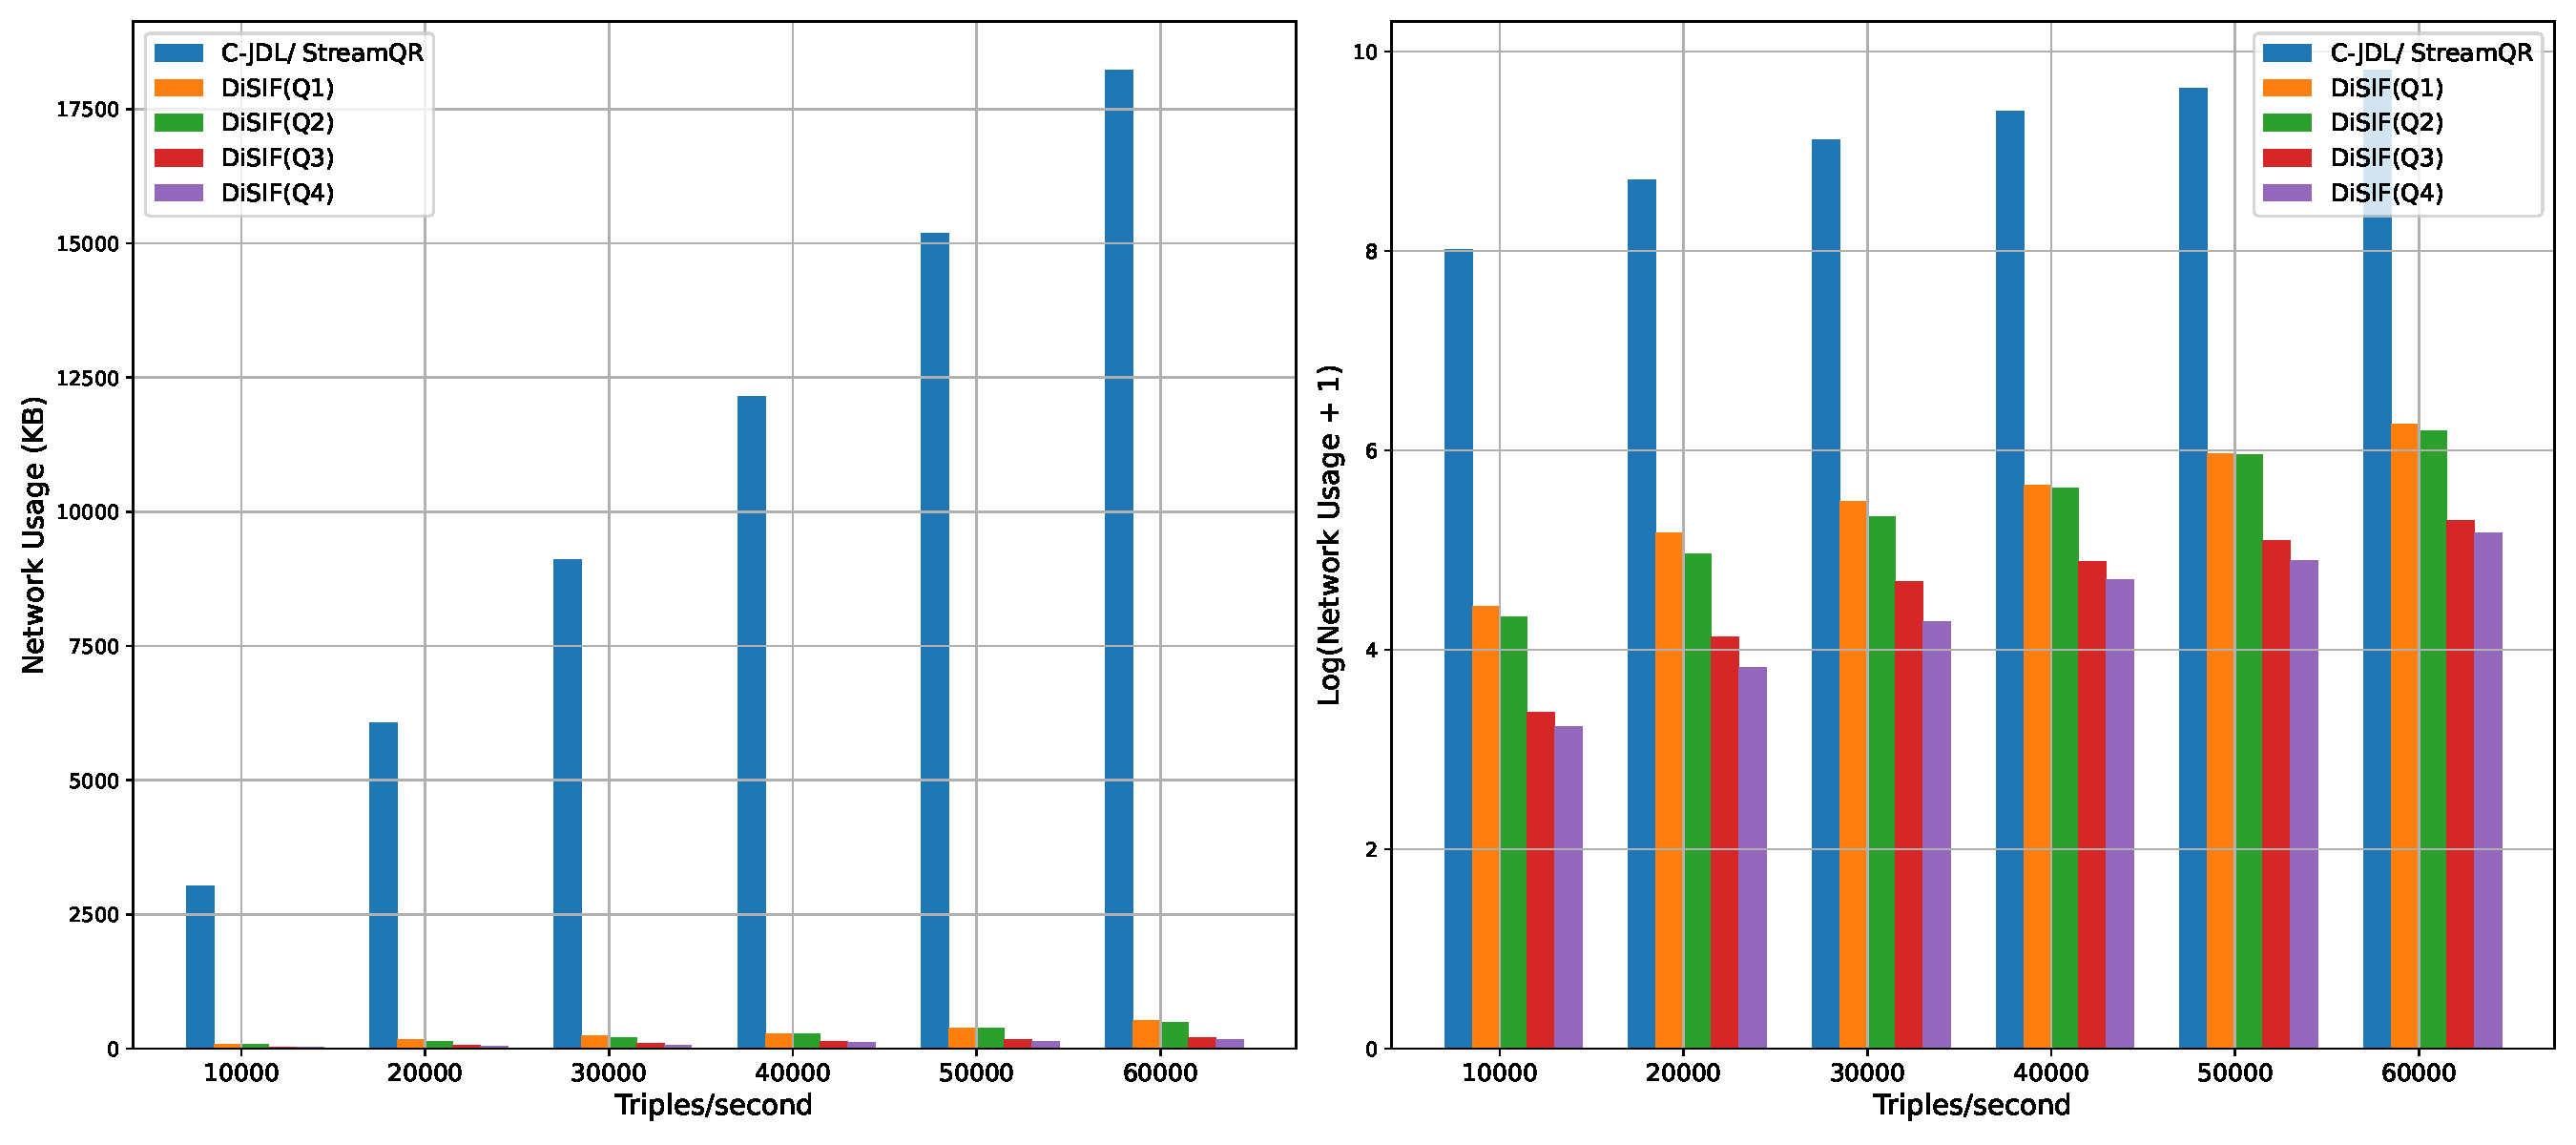
\includegraphics[width=0.5\textwidth]{Network_Usage_vs_Log_vs_Triples.pdf}
  \caption{Network usage comparison for different stream rates}
  \label{fig:networkLoad}
\end{figure}




As observed in Figure \ref{fig:networkLoad} , the volume of messages sent over the 
network wih Kafka in the C-JDL/StreamQR approaches is significantly higher compared
 to DiSIF approach.


In C-JDL/StreamQR approaches, all raw RDF data must be transmitted from worker nodes to
 the master node, resulting in a substantial network load. 
In contrast, the DiSIF method involves performing local computations and query executions
 on the worker nodes, with only the processed results—comprising much smaller message
  volumes—being transmitted to the master node.

Furthermore, as the data streaming rate increases, the number of messages sent also rises,
 highlighting the distinction between C-JDL/StreamQR approaches and DiSIF. 
Additionally, as the complexity of the queries increases  ($Q_1$< $Q_2$< $Q_3$< $Q_4$),
 fewer messages are sent in the network. In contrast, with C-JDL/StreamQR approaches,
  there is no significant difference in the volume of sent messages with respect to the
   complexity of the queries.



\subsection{Memory Consumption Perspective}


In terms of memory consumption, we employ the following two formulas to calculate the memory requirements for executing query $Q_m$ in both centralized and distributed approaches:

\begin{equation}
\text{Mem}_c(Q_i) = M_{Q_i Q_m} > M_{Q_i} + M_{Q_m}
\end{equation}

\begin{equation}
\text{Mem}_d(Q_i) = \max(M_{Q_i}, M_{Q_m})
\end{equation}

As observed, $M_{Q_i Q_m}$ signifies the amount of memory required when executing $Q_m$ and $Q_i$ sequentially on a master node. In both approaches, memory consumption for data transmission is neglected.

In the centralized approach, the sequential execution of queries $Q_i$ and $Q_m$ results in the generation of intermediate data in the memory of the master node. This leads to higher memory consumption ($\text{Mem}_c(Q_i Q_m)$) compared to the sum of individual memory consumptions ($M_{Q_i} + M_{Q_m}$).

However, in the distributed approach, since queries $Q_i$ and $Q_m$ are executed in parallel on different nodes, the memory consumption is equal to the maximum of the memory requirements for $Q_i$ and $Q_m$ in both worker and master nodes.

Next, we will analyze the distributed and centralized JDL methods in terms of memory
 consumption for executing query $Q_m$ on the master node.
%======================
\begin{figure}[t] % First figure
  \centering
  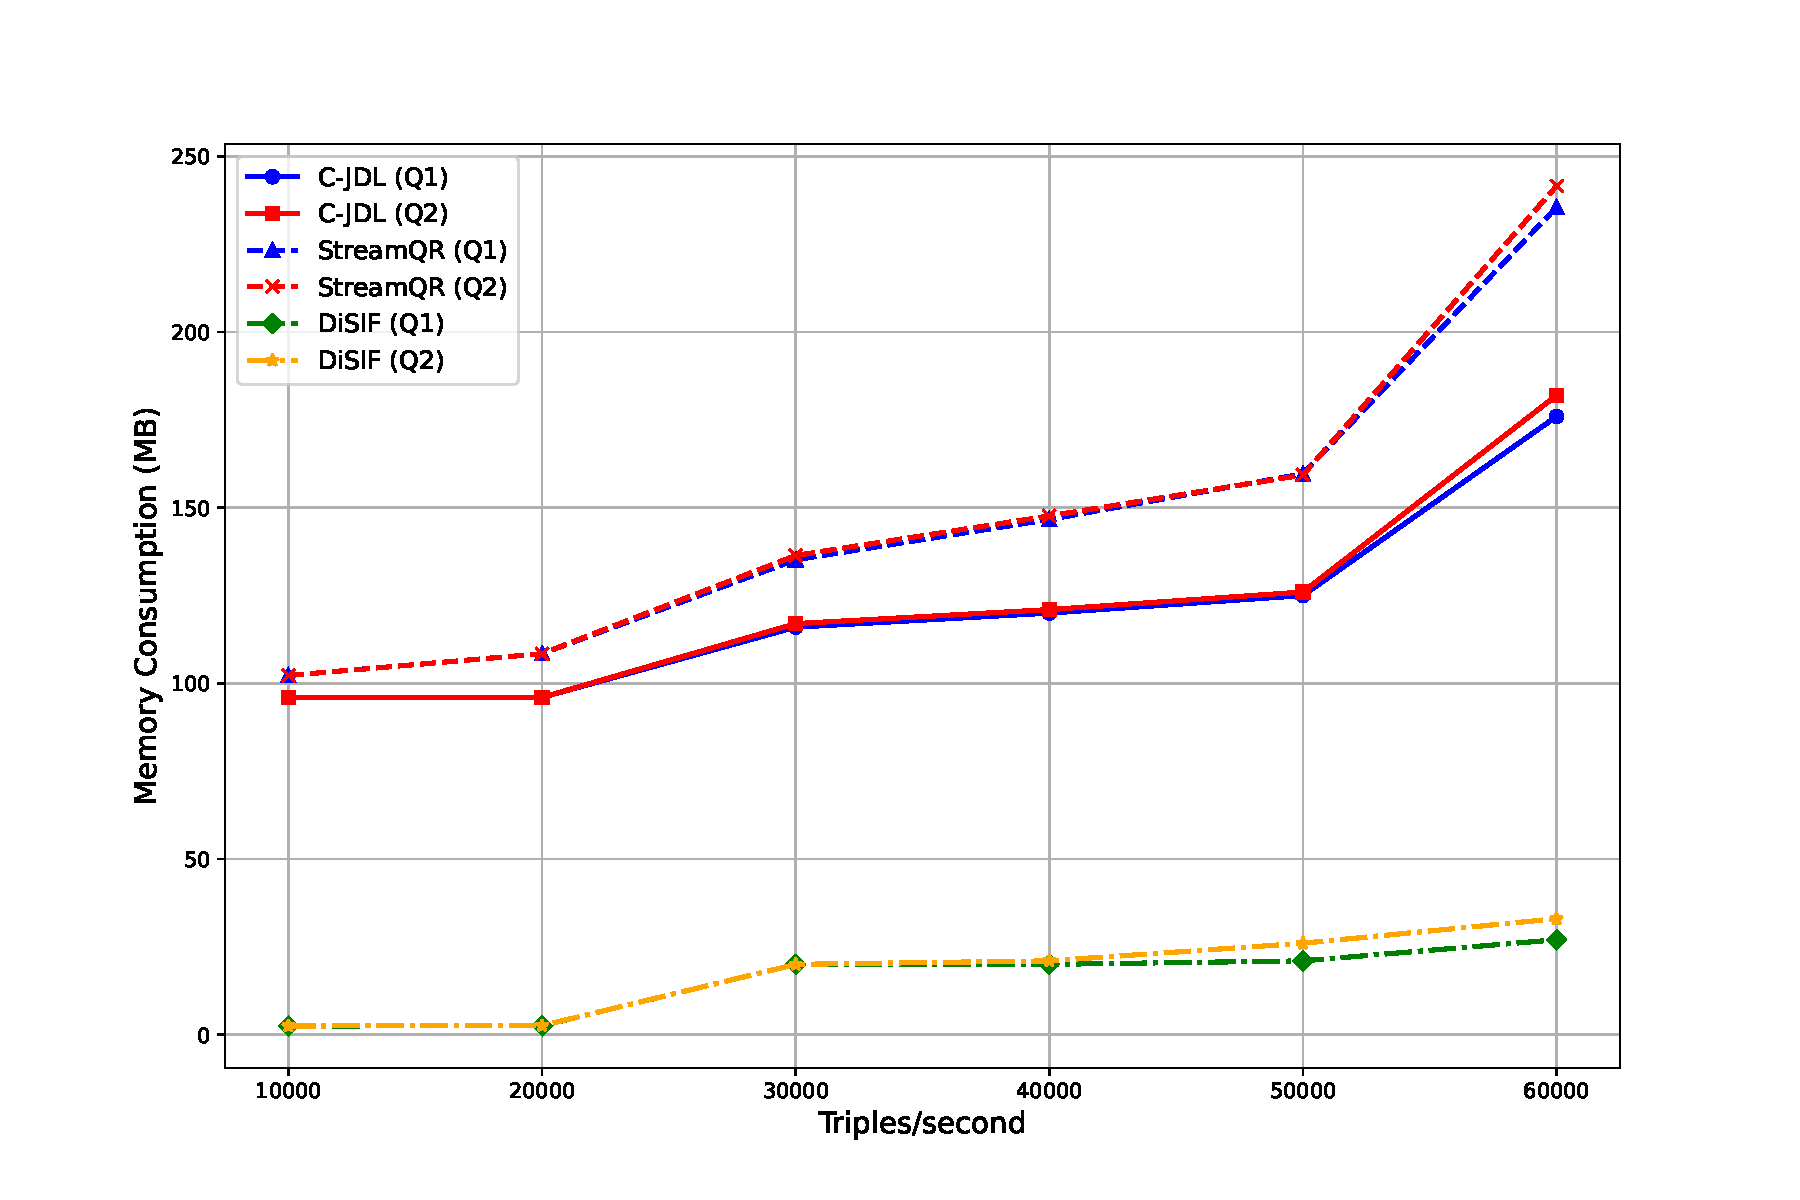
\includegraphics[width=0.8\columnwidth]{Memory_Consumption_vs_Stream_Rate_Linear_Enhanced_Q1Q2.pdf}
  \caption{Memory consumption for a single stream receiver node (Linear Scale) for Q1 and Q2}
  \label{fig:Memexperiment1}
\end{figure}

\begin{figure}[t] % Second figure
  \centering
  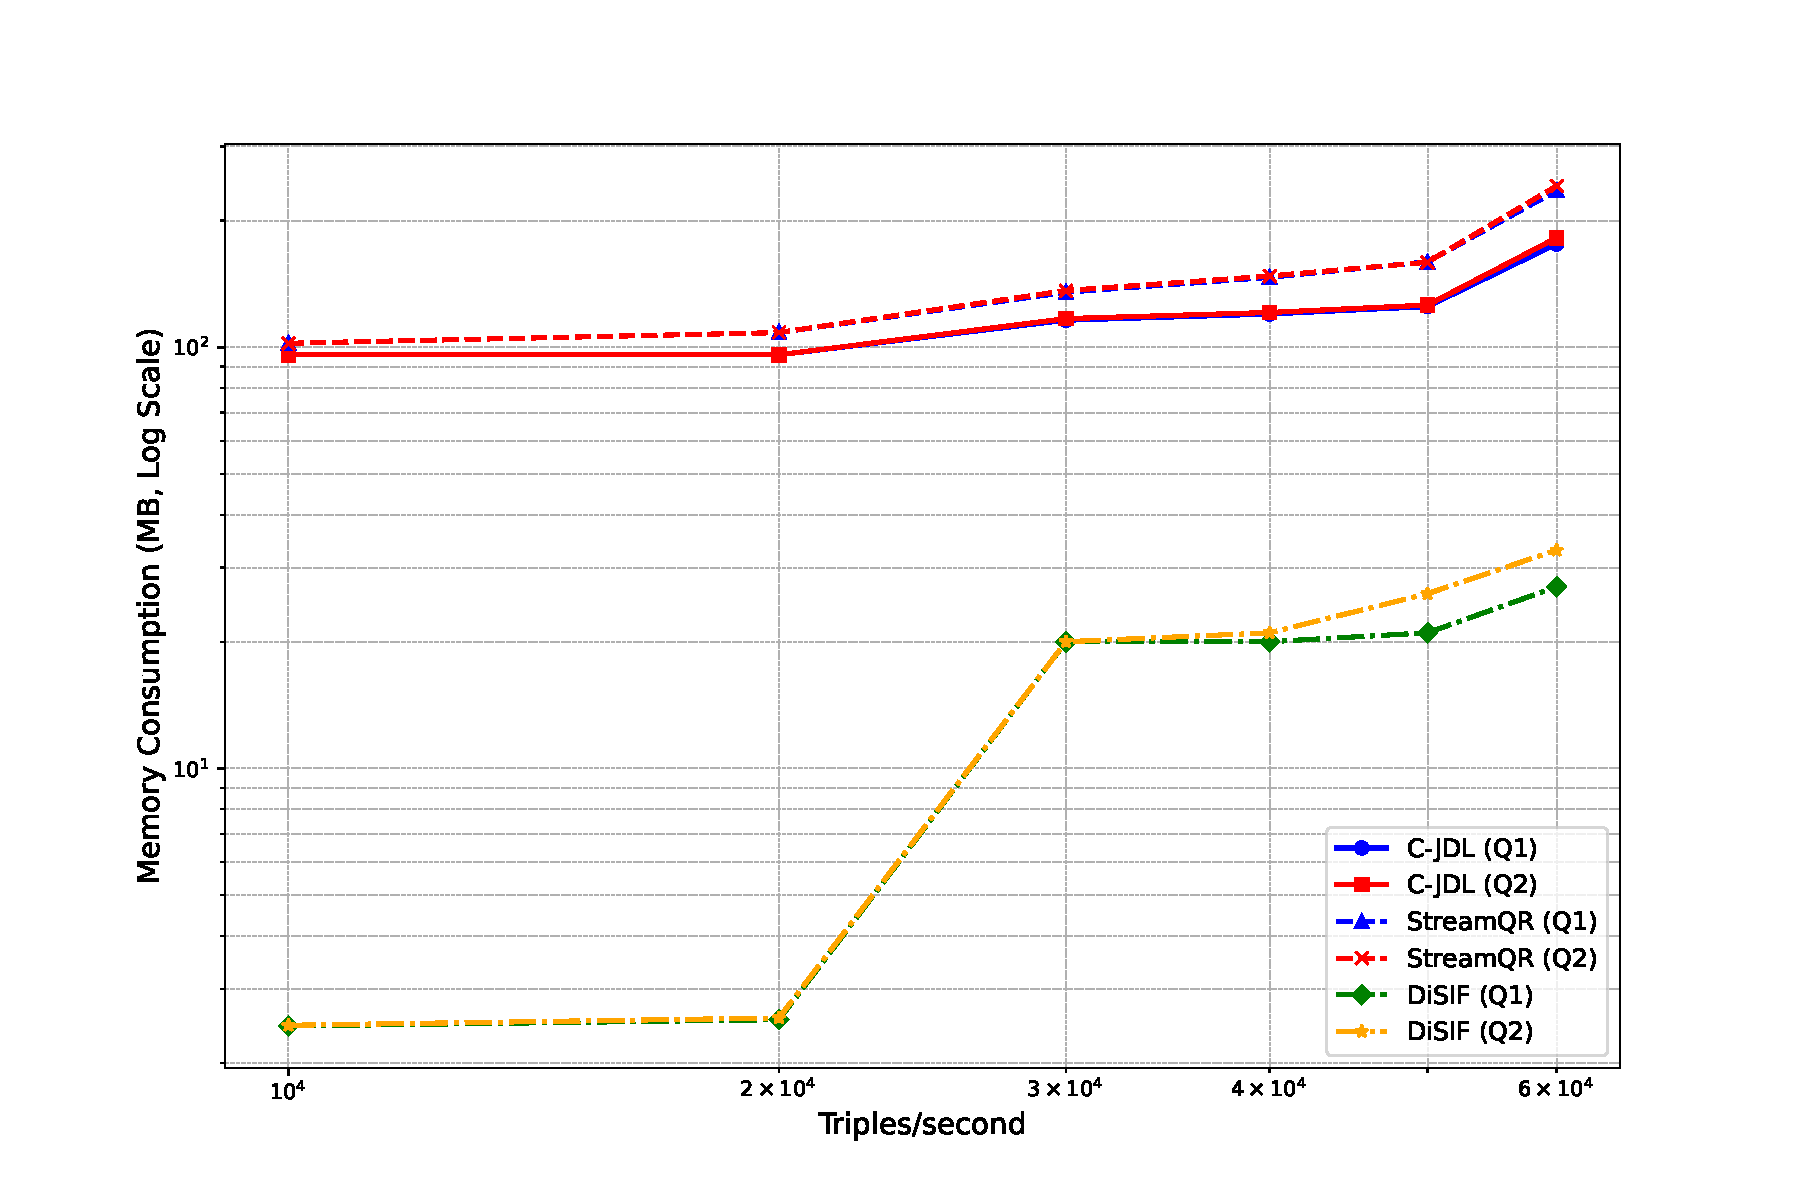
\includegraphics[width=0.8\columnwidth]{Memory_Consumption_vs_Stream_Rate_Log_Enhanced_Q1Q2.pdf}
  \caption{Memory consumption for a single stream receiver node (Log Scale) for Q1 and Q2}
  \label{fig:Memexperiment11}
\end{figure}

\begin{figure}[t] % Third figure
  \centering
  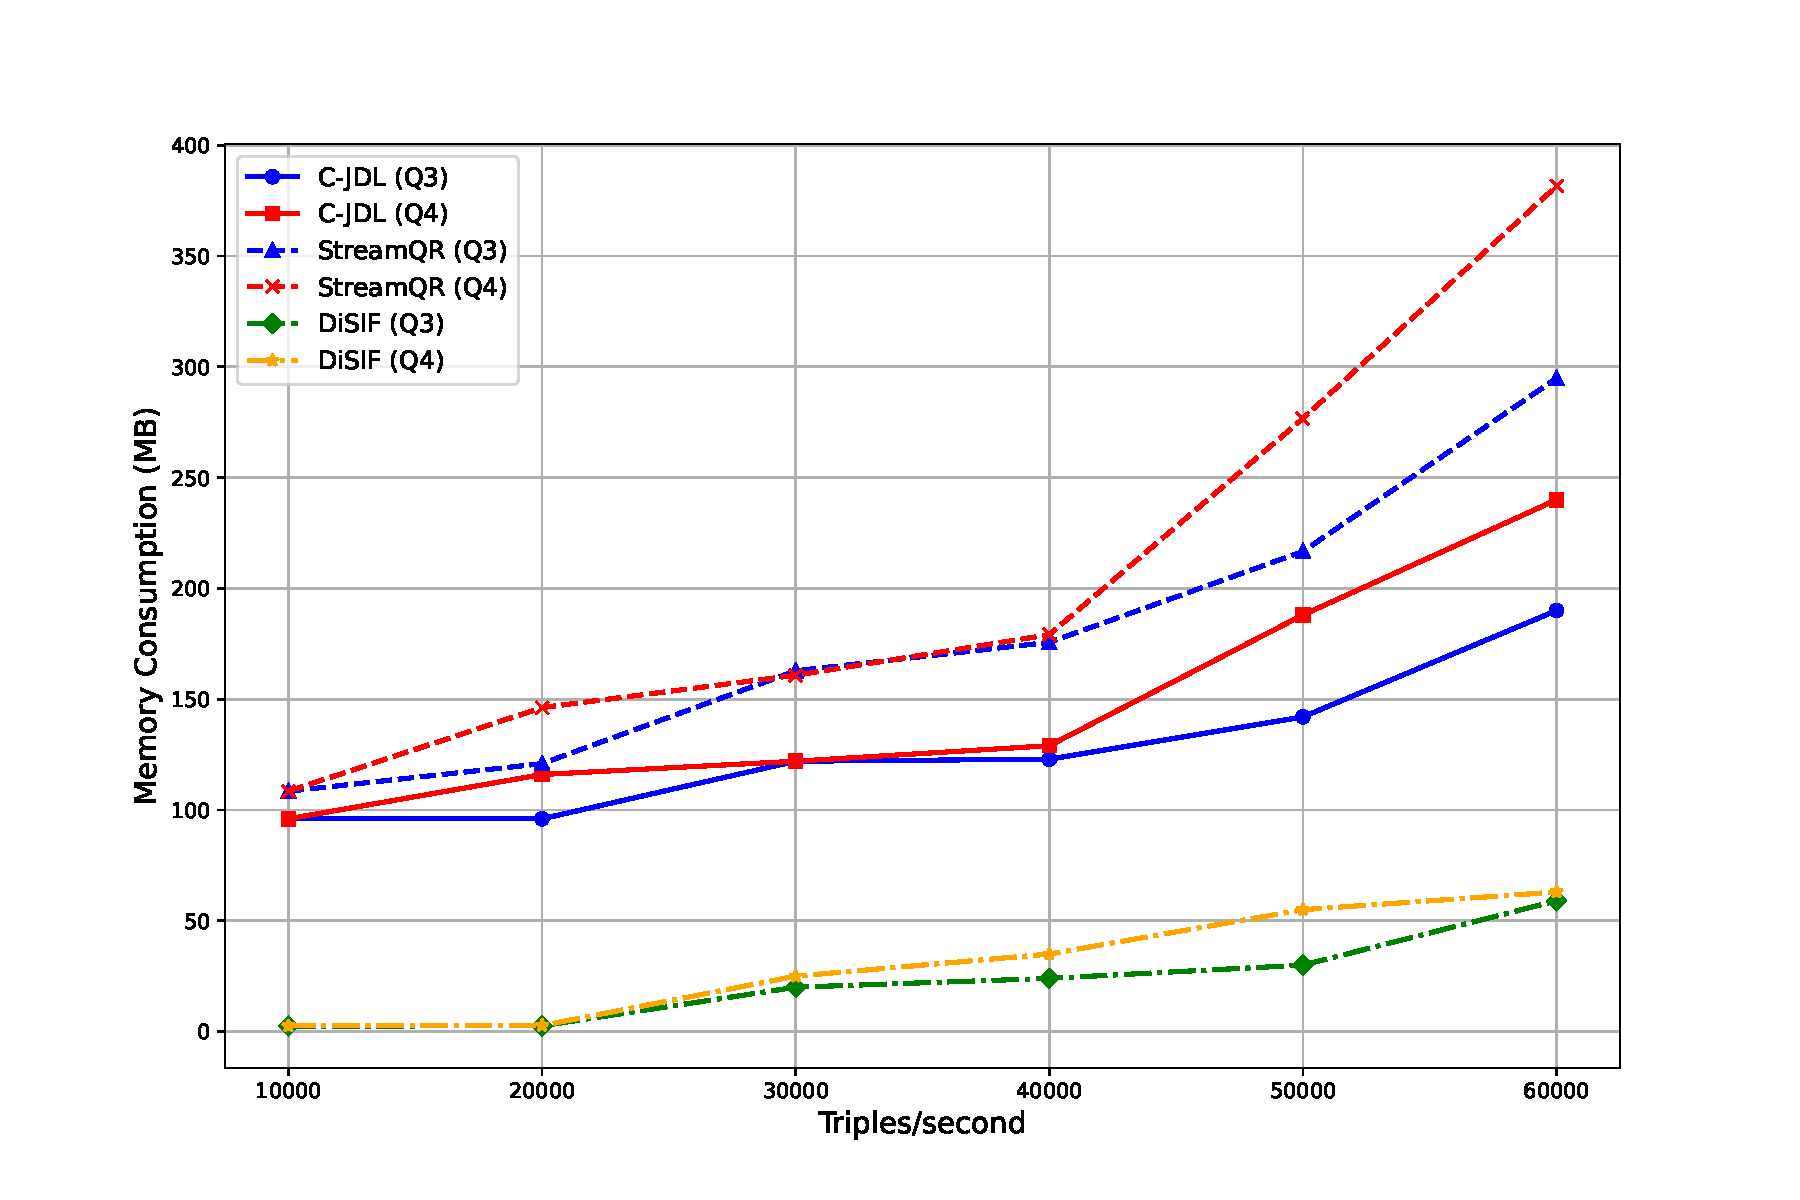
\includegraphics[width=0.8\columnwidth]{Memory_Consumption_vs_Stream_Rate_Linear_Enhanced_Q3Q4.pdf}
  \caption{Memory consumption for a single stream receiver node (Linear Scale) for Q3 and Q4}
  \label{fig:Memexperiment2}
\end{figure}

\begin{figure}[t] % Fourth figure
  \centering
  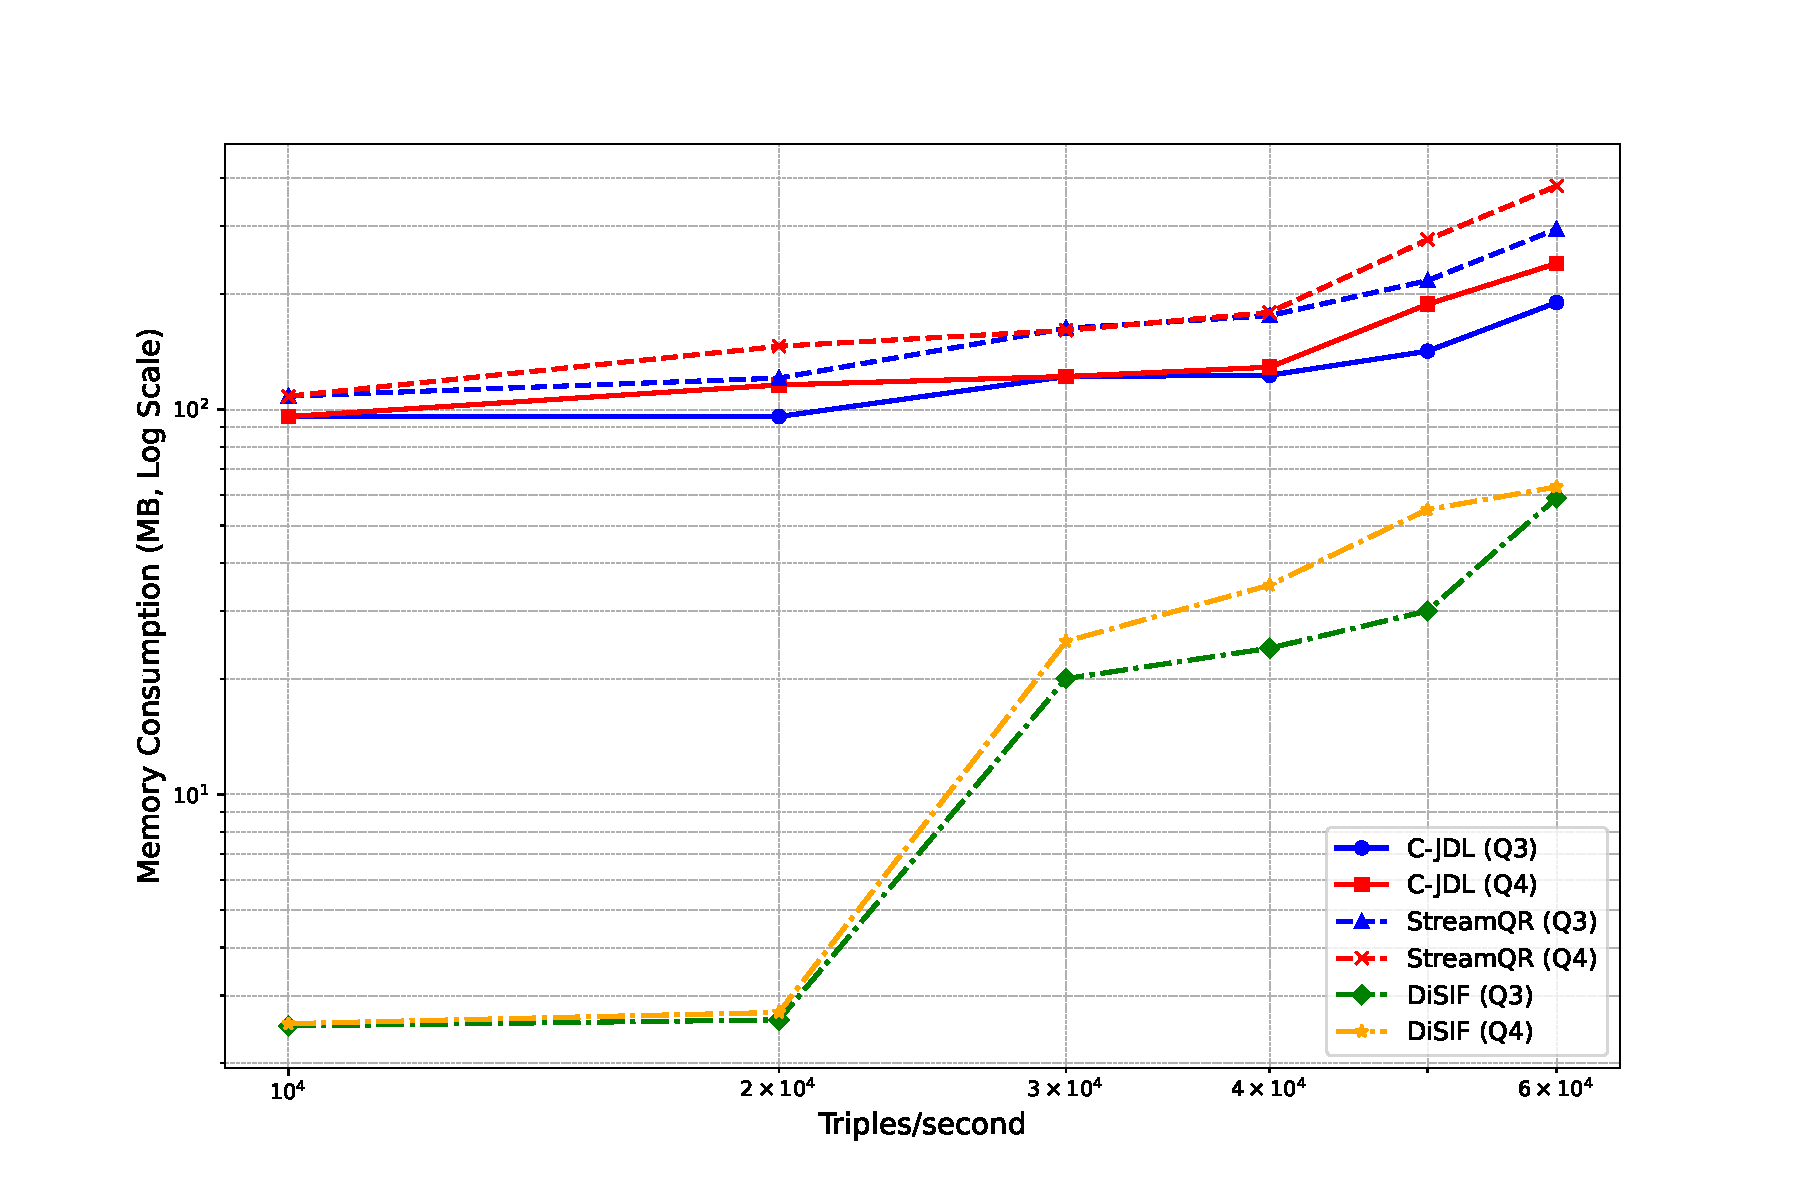
\includegraphics[width=0.8\columnwidth]{Memory_Consumption_vs_Stream_Rate_Log_Enhanced_Q3Q4.pdf}
  \caption{Memory consumption for a single stream receiver node (Log Scale) for Q3 and Q4}
  \label{fig:Memexperiment22}
\end{figure}
  %=================

% \begin{figure*}
%   \centering
%   \begin{subfigure}{0.45\textwidth}
%     \centering
%     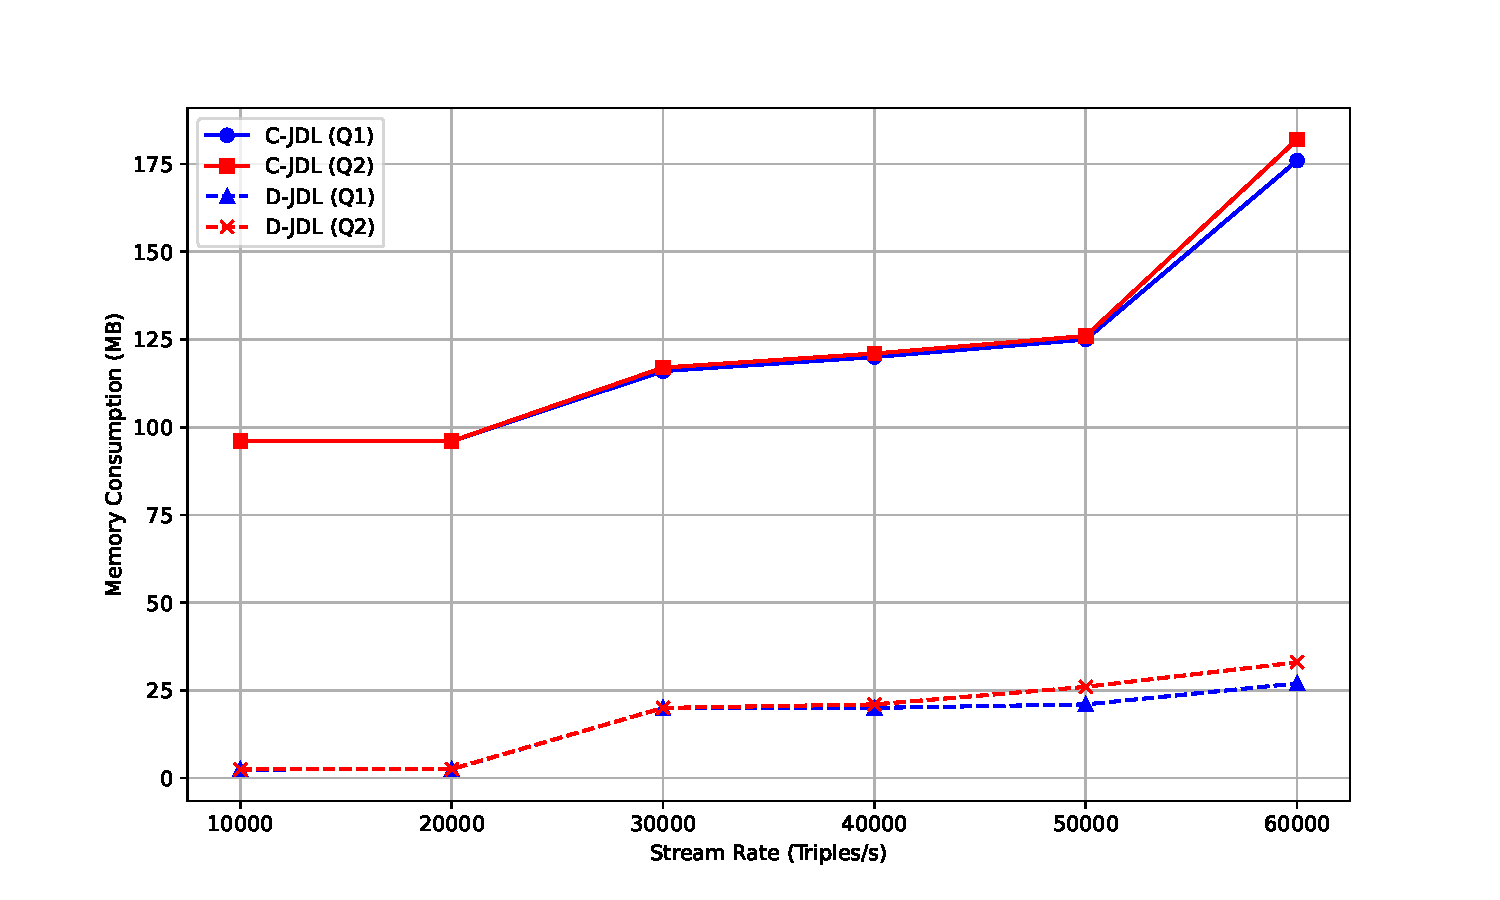
\includegraphics[width=\textwidth]{Memory_Consumption_Q1Q2.pdf}
%     \subcaption{A single stream receiver node}
%     \label{fig:Memexperiment1}
%   \end{subfigure}
%   \hfill
%   \begin{subfigure}{0.45\textwidth}
%     \centering
%     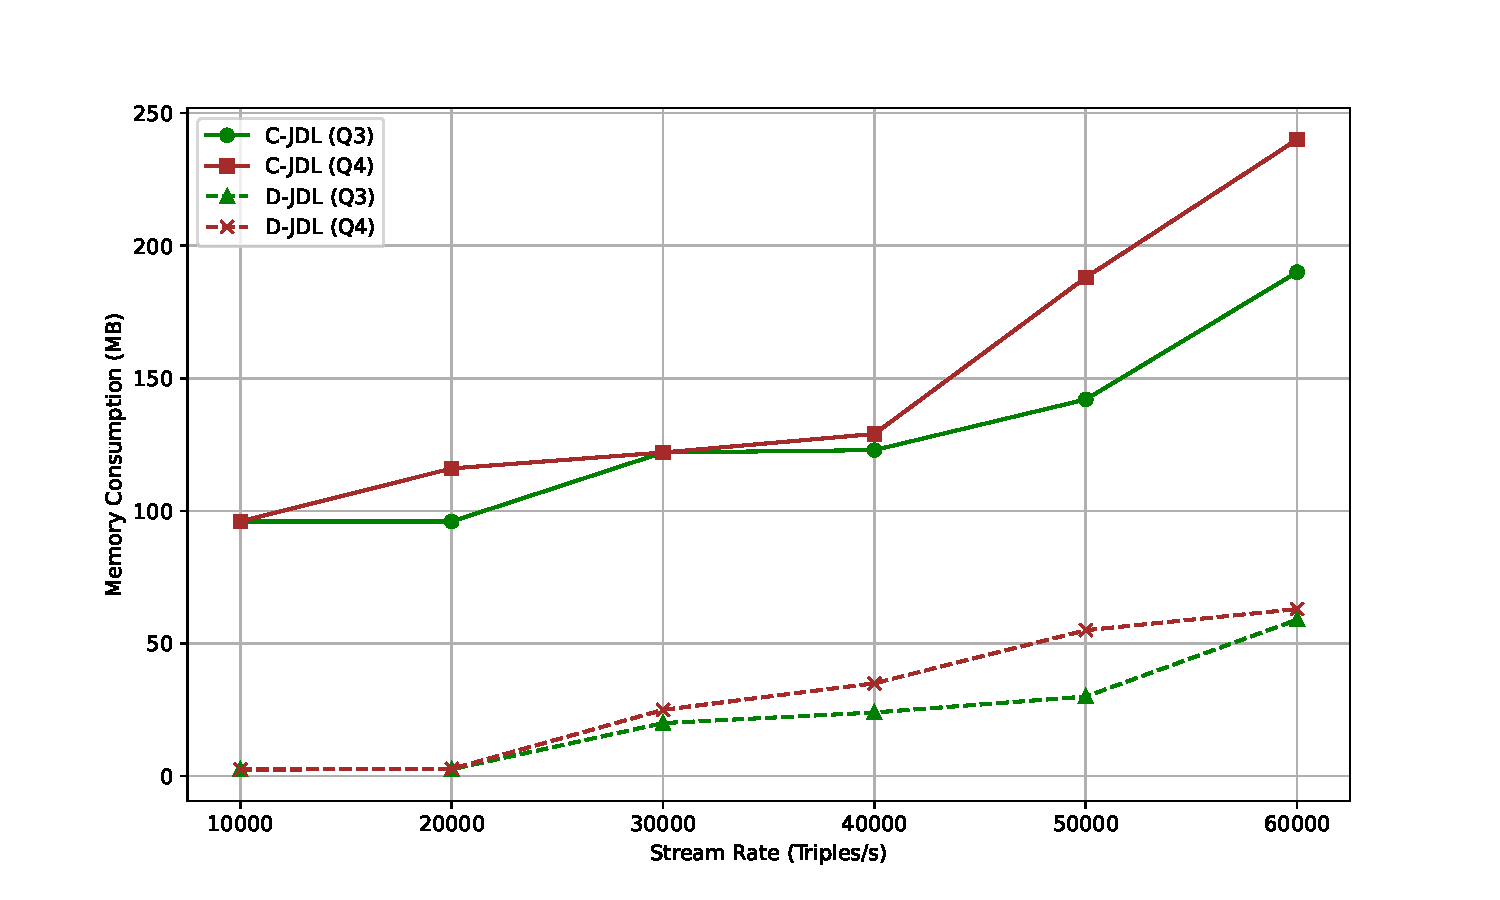
\includegraphics[width=\textwidth]{Memory_Consumption_Q3Q4.pdf}
%     \subcaption{Multiple concurrent stream receiver nodes}
%     \label{fig:Memexperiment2}
%   \end{subfigure}

%   \caption{Memory consumption for different stream reciever nodes}
%   \label{fig:Memexperiment1234}
% \end{figure*}


The StreamQR method, due to the aggregation of queries and the execution of a single
 large query (expanded query), can have higher memory consumption compared
  to the C-JDL method. The execution of this large query may require significant
   memory to process all the input data simultaneously and store intermediate results.
    Managing and processing the aggregated query, along with handling large volumes
     of intermediate data and results, can substantially increase memory usage in StreamQR.


In contrast, the C-JDL method manages memory separately for each query.
 Memory is temporarily released after each query's execution, as memory is only used 
 for the results and processing of individual queries. Despite this, centralized processing
  in C-JDL can still result in high memory usage when handling more complex queries,
   but it is generally lower than StreamQR because queries are executed individually rather
    than aggregated.


As shown in Figures \ref{fig:Memexperiment1} and \ref{fig:Memexperiment11}, memory consumption for executing queries
 $Q_1$ and $Q_2$ in the C-JDL is over four times greater than in
  the DiSIF. This occurs because, in the C-JDL,
   $Q_1$ (or $Q_2$) must be processed to generate outputs stored in the master node's memory,
    which are then used as input for query $Q_m$ to obtain the final results.
     As a result, memory usage in the C-JDL is significantly higher compared to
      the DiSIF.


Query $Q_2$, due to its use of aggregator functions such as GroupBy and Having,
 requires more memory consumption compared to $Q_1$.

On the other hand, Figures \ref{fig:Memexperiment2} and \ref{fig:Memexperiment22}, show that memory consumption
 for queries $Q_3$ and $Q_4$ in C-JDL and StreamQR is significantly higher than 
 in DiSIF approach. This increase is due to the use of AVG functions 
 and CONTAINS, which can elevate memory usage. Storing the outputs in
  memory and then executing $Q_m$ on these outputs substantially increases memory
   consumption for $Q_3$ and $Q_4$ in C-JDL and StreamQR compared
    to DiSIF approach.


Moreover, Figures \ref{fig:Memexperiment1} and \ref{fig:Memexperiment2} demonstrate
 that the AVG and CONTAINS functions in queries $Q_3$ and $Q_4$ can significantly
  increase memory consumption, particularly when data transmission rates exceed 40,000
   triples per second in C-JDL and StreamQR. Additionally, as the data transmission rate
    increases, memory consumption for $Q_4$ surpasses that of $Q_3$, a trend that becomes
     noticeable when data transmission rates surpass 40,000 triples per second.

%\begin{figure}[h]
%    \centering
%    \includegraphics[width=0.8\textwidth]{network_load_comparison.png}
%    \caption{Network Load Comparison}
%\end{figure}
%
%???????????
%# Experiments
%?????????
% \section{Discussion}

\section{Conclusion and future works}
This study introduces a novel distributed semantic JDL fusion model tailored for smart city applications, leveraging a three-layer architecture consisting of edge, fog, and cloud layers. Our framework addresses the limitations of centralized fusion models, particularly the inefficiencies associated with processing vast volumes of heterogeneous data in smart cities. Key benefits of our approach include: 

Enhanced Network Efficiency: By performing low-level data processing at the edge and transmitting only the processed results to higher layers, our model significantly reduces network load and optimizes bandwidth usage.

Reduced Query Execution Time: The ability to decompose complex queries into independent and dependent sub-queries, executed in parallel across different layers, ensures faster query responses and improves overall system responsiveness. 

Improved Data Privacy: Our distributed approach minimizes the need to transmit raw data across the network, thereby enhancing data privacy and security.

Resource Optimization: Distributing computational loads across multiple nodes and layers reduces memory consumption and improves processing efficiency, making the system more scalable and robust.

Our evaluations demonstrate that the distributed JDL model outperforms traditional centralized approaches by reducing network load, decreasing query execution time, and optimizing memory usage. The integration of horizontal and vertical fusion techniques allows for effective management of both heterogeneous and homogeneous data, thus improving the reliability and accuracy of decision-making processes in smart cities.

Furthermore, the DiSIF framework supports real-time, decentralized decision-making, which is critical for addressing the diverse and dynamic needs of urban environments. The innovative approach of combining data fusion at different layers with a distributed query execution model provides a comprehensive solution for the complex data management challenges faced by smart cities.

Future research will focus on refining the model, exploring its application across various smart city scenarios, and addressing new challenges related to large-scale data fusion and real-time processing. The DiSIF framework represents a significant advancement in the efficient management and utilization of smart city data, paving the way for more responsive, adaptive, and intelligent urban systems.

\section{Declaration of competing interest}

The authors declare that they have no known competing financial
interests or personal relationships that could have appeared
to influence the work reported in this paper.

%\section{Data availability}   (mitavanim nadashte bashim)

%\section*{Appendix. Basic graph pattern}

% \section*{Acknowledgments}   (ma nadarim)

% Acknowledgments (if any) go here


%\section{References}

%\bibliographystyle{ieeetr}
%\bibstyle{ieeetr}
\bibliographystyle{plain}

\bibliography{thesis_bib} % Replace 'your_bibliography_file' with the name of your .bib file



% Start the appendix
\appendix

\section{Queries}
\label{sec:AppendixQueries}
% Content of Appendix B


\textbf{Query \(Q_m\)}
\begin{verbatim}
REGISTER QUERY Traffic AS
    PREFIX ex: <http://myexample.org/>
    PREFIX loc: <https://location.com/>
    PREFIX stat: <https://status.com/>
    PREFIX cnt: <https://cntVehicles/>
    PREFIX concept: <https://concept.com/>

    SELECT ?s
    FROM STREAM <streamIRI_new>
                 [RANGE 3s STEP 1s]
    WHERE {
        ?s concept:congestion ?o .
    }
    GROUP BY (?s)
    HAVING (COUNT(?o) > 3);
\end{verbatim}



\textbf{Query 1}

\begin{verbatim}

REGISTER QUERY CongestionDetect AS
PREFIX ex: <http://example.org/>
PREFIX geo: <http://www.w3.org/2003/
            01/geo/wgs84_pos#>
PREFIX stat: <https://status.com/>
PREFIX concept: <https://concept.com/>

CONSTRUCT {
  ?location concept:congestion "congestion" .
}
FROM STREAM <https://www.wtlab.com/TrafficStream>
            [RANGE 3s STEP 1s]
WHERE {
  ?vehicle geo:location ?location ;
           concept:speed ?speedValue ;
           ex:timestamp ?timestamp .
  FILTER(?speed < 50)
}

\end{verbatim}

\textbf{Query 2:}

\begin{verbatim}

    REGISTER QUERY CongestionDetect AS
    PREFIX ex: <http://example.org/>
    PREFIX geo: <http://www.w3.org/2003/01/
                geo/wgs84_pos#>
    PREFIX concept: <https://concept.com/>

    CONSTRUCT {
      ?location concept:congestion "congestion" .
    }
    FROM STREAM <https://www.wtlab.com/TrafficStream>
                 [RANGE 3s STEP 1s]
    WHERE {
      ?vehicle geo:location ?location ;
               concept:speed ?speedValue ;
               ex:timestamp ?timestamp .
      FILTER(?speed < 50)
    }
    GROUP BY ?location
    HAVING (COUNT(?vehicle) > 3)
    ORDER BY ASC(?location)
\end{verbatim}

\textbf{Query 3:}
\begin{verbatim}
REGISTER QUERY CongestionDetect AS
PREFIX ex: <http://example.org/>
PREFIX geo: <http://www.w3.org/2003/01/
            geo/wgs84_pos#>
PREFIX stat: <https://status.com/>
PREFIX concept: <https://concept.com/>

CONSTRUCT {
  ?location concept:congestion "congestion" .
  ?location stat:avgSpeed ?avgLocation .
}
FROM STREAM <https://www.wtlab.com/TrafficStream> 
            [RANGE 3s STEP 1s]
WHERE {
  ?vehicle geo:location ?location ;
           concept:speed ?speedValue ;
           ex:timestamp ?timestamp .

  FILTER(?speed < 50)
  FILTER (CONTAINS(str(?location), "2") ||
          CONTAINS(str(?location), "3") ||
          CONTAINS(str(?location), "1"))
}
GROUP BY ?location
HAVING (COUNT(?vehicle) > 1)
BIND(AVG(?speed) AS ?avgLocation)
ORDER BY ASC(?location)
\end{verbatim}

\textbf{Query 4:}

\begin{verbatim}
REGISTER QUERY CongestionDetect AS
PREFIX ex: <http://example.org/>
PREFIX geo: <http://www.w3.org/2003/01/
            geo/wgs84_pos#>
PREFIX stat: <https://status.com/>
PREFIX concept: <https://concept.com/>

CONSTRUCT {
  ?location concept:congestion "congestion" .
  ?location stat:avgSpeed ?avgLocation .
}
FROM STREAM <https://www.wtlab.com/TrafficStream> 
            [RANGE 3s STEP 1s]
WHERE {
  ?vehicle geo:location ?location ;
           concept:speed ?speedValue ;
           ex:timestamp ?timestamp .

  FILTER(?speed < 50)
  FILTER (CONTAINS(str(?location), "2") ||
          CONTAINS(str(?location), "3") ||
          CONTAINS(str(?location), "1"))
    UNION
    {
    ?vehicle geo:location ?location ;
                ex:speed ?speed ;
                ex:timestamp ?timestamp .
    FILTER(?speed < 50)
    FILTER (CONTAINS(str(?location), "4"))
    }
}
GROUP BY ?location
HAVING (COUNT(?vehicle) > 1)
BIND(AVG(?speed) AS ?avgLocation)
ORDER BY ASC(?location)
\end{verbatim}
\end{document} 